%==============================================================================
% Masters Thesis Document
% This document template is adapted by Lester James V. Miranda
% for his Masters thesis in Waseda University.
%
% Using LaTeX Template Version 2.5 (27/8/17)
% The template was downloaded from:
% http://www.LaTeXTemplates.com
%
% Version 2.x major modifications by:
% Vel (vel@latextemplates.com)
%
% This template is based on a template by:
% Steve Gunn (users.ecs.soton.ac.uk/srg/softwaretools/document/templates/)
% Sunil Patel (sunilpatel.co.uk/thesis-template/)
%
% This file is part of thesis-manuscript.
%
% thesis-mansucript is free software: you can redistribute it and/or modify
% it under the terms of the GNU General Public License as published by
% the Free Software Foundation, either version 3 of the License, or
% (at your option) any later version.
%
% thesis-manuscript is distributed in the hope that it will be useful,
% but WITHOUT ANY WARRANTY; without even the implied warranty of
% MERCHANTABILITY or FITNESS FOR A PARTICULAR PURPOSE.  See the
% GNU General Public License for more details.
%
% You should have received a copy of the GNU General Public License
% along with thesis-manuscript.  If not, see <http://www.gnu.org/licenses/>.
%
%==============================================================================

%------------------------------------------------------------------------------
%	PACKAGES AND OTHER DOCUMENT CONFIGURATIONS
%------------------------------------------------------------------------------

\documentclass[11pt,
            english,
            twoside,
            liststotoc,
            toctotoc,
            singlespacing,
            headsepline,
            consistentlayout]{style}
\usepackage[utf8]{inputenc}
%\usepackage[T1]{fontenc}
%\usepackage{mathptmx}
\usepackage[backend=biber,style=authoryear,natbib=true]{biblatex}
\usepackage[autostyle=true]{csquotes}
\usepackage{enumitem}
\usepackage{amsmath}
\usepackage{amssymb}
\usepackage{wrapfig}
\usepackage{algorithm}
\usepackage{algpseudocode}
\usepackage{threeparttable}
\usepackage{footmisc}
\usepackage{listings}
\usepackage{siunitx}
\usepackage{ntheorem}
\usepackage{mdframed}
\usepackage{mathtools}
\usepackage{array}
\usepackage{subcaption}
\usepackage{appendix}

\addbibresource{bibliography.bib}

%------------------------------------------------------------------------------
%	DEFINITION
%------------------------------------------------------------------------------
\theoremstyle{definition}
\theoremheaderfont{\bfseries}
\newmdtheoremenv[
    leftmargin=40, rightmargin=20,
    backgroundcolor=gray!20, linecolor=gray!20,
    innertopmargin=10,
    ntheorem
]{definition}{Definition}[section]
%\newtheorem{definition}{Definition}[section]

%------------------------------------------------------------------------------
%   SIUNITX SETTINGS
%------------------------------------------------------------------------------
% set-up numbers
\sisetup{
    output-exponent-marker=\ensuremath{\mathrm{e}},
    round-mode=places, round-precision=2,
    separate-uncertainty=false,
    detect-weight=true,
    detect-family=true,
    detect-inline-weight=math
}
\newcommand{\hg}{\bfseries}

%------------------------------------------------------------------------------
%	OTHER SETTINGS
%------------------------------------------------------------------------------
\definecolor{gray}{gray}{0.5}
\colorlet{commentcolour}{green!50!black}

\colorlet{stringcolour}{red!60!black}
\colorlet{keywordcolour}{magenta!90!black}
\colorlet{exceptioncolour}{yellow!50!red}
\colorlet{commandcolour}{blue!60!black}
\colorlet{numpycolour}{blue!60!green}
\colorlet{literatecolour}{magenta!90!black}
\colorlet{promptcolour}{green!50!black}
\colorlet{specmethodcolour}{violet}

\newcommand*{\framemargin}{3ex}

\newcommand*{\literatecolour}{\textcolor{literatecolour}}

\newcommand*{\pythonprompt}{\textcolor{promptcolour}{{>}{>}{>}}}


\lstdefinestyle{mypython}{
%\lstset{
%keepspaces=true,
language=python,
showtabs=true,
tab=,
tabsize=2,
basicstyle=\ttfamily\footnotesize,%\setstretch{.5},
stringstyle=\color{stringcolour},
showstringspaces=false,
alsoletter={1234567890},
otherkeywords={\%, \}, \{, \&, \|},
keywordstyle=\color{keywordcolour}\bfseries,
emph={and,break,class,continue,def,yield,del,elif ,else,%
except,exec,finally,for,from,global,if,import,in,%
lambda,not,or,pass,print,raise,return,try,while,assert,with},
emphstyle=\color{blue}\bfseries,
emph={[2]True, False, None},
emphstyle=[2]\color{keywordcolour},
emph={[3]object,type,isinstance,copy,deepcopy,zip,enumerate,reversed,list,set,len,dict,tuple,xrange,append,execfile,real,imag,reduce,str,repr},
emphstyle=[3]\color{commandcolour},
emph={Exception,NameError,IndexError,SyntaxError,TypeError,ValueError,OverflowError,ZeroDivisionError},
emphstyle=\color{exceptioncolour}\bfseries,
%upquote=true,
morecomment=[s]{"""}{"""},
commentstyle=\color{commentcolour}\slshape,
%emph={[4]1, 2, 3, 4, 5, 6, 7, 8, 9, 0},
emph={[4]ode, fsolve, sqrt, exp, sin, cos,arctan, arctan2, arccos, pi,  array, norm, solve, dot, arange, isscalar, max, sum, flatten, shape, reshape, find, any, all, abs, plot, linspace, legend, quad, polyval,polyfit, hstack, concatenate,vstack,column_stack,empty,zeros,ones,rand,vander,grid,pcolor,eig,eigs,eigvals,svd,qr,tan,det,logspace,roll,min,mean,cumsum,cumprod,diff,vectorize,lstsq,cla,eye,xlabel,ylabel,squeeze},
emphstyle=[4]\color{numpycolour},
emph={[5]__init__,__add__,__mul__,__div__,__sub__,__call__,__getitem__,__setitem__,__eq__,__ne__,__nonzero__,__rmul__,__radd__,__repr__,__str__,__get__,__truediv__,__pow__,__name__,__future__,__all__},
emphstyle=[5]\color{specmethodcolour},
emph={[6]assert,yield},
emphstyle=[6]\color{keywordcolour}\bfseries,
emph={[7]range},
emphstyle={[7]\color{keywordcolour}\bfseries},
% emph={[7]self},
% emphstyle=[7]\bfseries,
literate=*%
{:}{{\literatecolour:}}{1}%
{=}{{\literatecolour=}}{1}%
{-}{{\literatecolour-}}{1}%
{+}{{\literatecolour+}}{1}%
{*}{{\literatecolour*}}{1}%
{**}{{\literatecolour{**}}}2%
{/}{{\literatecolour/}}{1}%
{//}{{\literatecolour{//}}}2%
{!}{{\literatecolour!}}{1}%
%{(}{{\literatecolour(}}{1}%
%{)}{{\literatecolour)}}{1}%
{[}{{\literatecolour[}}{1}%
{]}{{\literatecolour]}}{1}%
{<}{{\literatecolour<}}{1}%
{>}{{\literatecolour>}}{1}%
{>>>}{\pythonprompt}{3}%
,%
%aboveskip=.5ex,
frame=trbl,
%frameround=tttt,
%framesep=.3ex,
rulecolor=\color{black!40},
%framexleftmargin=\framemargin,
%framextopmargin=.1ex,
%framexbottommargin=.1ex,
%framexrightmargin=\framemargin,
%framexleftmargin=1mm, framextopmargin=1mm, frame=shadowbox, rulesepcolor=\color{blue},#1
%frame=tb,
backgroundcolor=\color{white},
breakindent=.5\textwidth,frame=single,breaklines=true%
%}
}



\setcounter{tocdepth}{1}
\setitemize{itemsep=-0.2em}        % Modify spacing between items
%\renewcommand{\arraystretch}{1.2}  % Stretch tables

% Command for algorithm INPUT and OUTPUT
\algnewcommand\algorithmicinput{\textbf{Input:}}
\algnewcommand\INPUT{\item[\algorithmicinput]}
\algnewcommand\algorithmicoutput{\textbf{Output:}}
\algnewcommand\OUTPUT{\item[\algorithmicoutput]}

% Set-up footnotes
%\renewcommand{\thefootnote}{\fnsymbol{footnote}}

% Item settings
\setlist{parsep=0pt, listparindent=\parindent}

% Math fonts set-up
\DeclareMathAlphabet{\mathcal}{OMS}{cmsy}{m}{n}
\SetMathAlphabet{\mathcal}{bold}{OMS}{cmsy}{b}{n}
\newcommand{\bigO}{\mathcal{O}}
\newcommand\given[1][]{\:#1\vert\:}
%------------------------------------------------------------------------------
%	MARGIN SETTINGS
%------------------------------------------------------------------------------

\geometry{
    paper=letterpaper, % Change to letterpaper for US letter
    inner=2.5cm, % Inner margin
    outer=3.8cm, % Outer margin
    bindingoffset=.5cm, % Binding offset
    top=1.5cm, % Top margin
    bottom=1.5cm, % Bottom margin
    showcrop
}

%------------------------------------------------------------------------------
%	THESIS INFORMATION
%------------------------------------------------------------------------------

\thesistitle{
    Autoencoder-based Feature Extraction Techniques for Protein Function
    Prediction
}
\supervisor{Dr. Jinglu Hu}
\degree{Master of Engineering}
\author{Lester James V. Miranda}
\addresses{}

\subject{Masters Thesis of Lester James V. Miranda}
\keywords{
    machine learning,
    bioinformatics,
    feature extraction,
    multilabel classification
}
\university{Waseda University}
\department{Graduate School of Information, Production, and Systems}
\group{Furuzuki Neurocomputing Systems Laboratory}
\faculty{Information Architecture}

\AtBeginDocument{
\hypersetup{pdftitle=\ttitle}
\hypersetup{pdfauthor=\authorname}
\hypersetup{pdfcreator=\authorname}
\hypersetup{pdfproducer=\authorname}
\hypersetup{pdfkeywords=\keywordnames}
\hypersetup{pdfsubject=\subject}
}

\begin{document}

\frontmatter

\pagestyle{plain}

%------------------------------------------------------------------------------
%	TITLE PAGE
%------------------------------------------------------------------------------

\begin{titlepage}
\begin{center}
\vspace*{.02\textheight}
{\LARGE \bfseries \ttitle}\vspace{2.5cm} % Thesis title

{\Large 44161652-3: \authorname} % Author name
\vfill 

{\normalsize \degreename} \\[2.5cm] % Degree

{\normalsize Supervisor: \supname} \\[2.5cm] % Supervisor's name

{\normalsize \groupname} \\        % Laboratory affilation
{\normalsize \facname}   \\        % Faculty affiliation
{\normalsize \deptname}  \\[0.5cm] % Departmental affiliation

{\normalsize \univname} \\[0.5cm] % University affiliation

{\normalsize \today} % Current date
\end{center}
\end{titlepage}

%------------------------------------------------------------------------------
%	SECOND TITLE PAGE
%------------------------------------------------------------------------------
\begin{titlepage}
\begin{center}
\thispagestyle{empty}
\vspace*{.02\textheight}
{\ttitle} \\[2.5cm] % Thesis title
{44161652-3: \authorname} \\[2.5cm] % Author name
{
    A thesis submitted to the Graduate School of \\
    Information, Production, and Systems\\
    Waseda University\\
    in partial fulfillment of the requirements for the degree of
} \\[1.2cm]

{\degreename} \\[2.5cm]
{Supervisor: \supname} \vfill
{\deptname}\\[1.0cm]
{\univname}\\[1.0cm]
{\today} \vfill


\includegraphics[width=0.25\textwidth]{wasedaLogo}\\[0.1cm]
{Copyright \textcopyright 2018 44161652-3: \authorname} \\[0.2cm]
All Rights Reserved
\end{center}
\end{titlepage}


%------------------------------------------------------------------------------
%	ABSTRACT PAGE
%------------------------------------------------------------------------------

\begin{abstract}
\addchaptertocentry{\abstractname} % Add the abstract to the table of contents

%=============================================================================
% Abstract
% Copyright (c) 2018. Lester James V. Miranda
%
% This file is part of thesis-manuscript.
%
% thesis-mansucript is free software: you can redistribute it and/or modify
% it under the terms of the GNU General Public License as published by
% the Free Software Foundation, either version 3 of the License, or
% (at your option) any later version.
%
% thesis-manuscript is distributed in the hope that it will be useful,
% but WITHOUT ANY WARRANTY; without even the implied warranty of
% MERCHANTABILITY or FITNESS FOR A PARTICULAR PURPOSE.  See the
% GNU General Public License for more details.
%
% You should have received a copy of the GNU General Public License
% along with thesis-manuscript.  If not, see <http://www.gnu.org/licenses/>.
%
% Created by: Lester James V. Miranda <ljvmiranda@gmail.com>
%=============================================================================

\par Protein function prediction is a fundamental task with applications in
medicine and healthcare. However, the cost and slow-pace of biochemical
techniques hinder this process, causing a major backlog to the number of
unannotated proteins we have today. Machine learning techniques are suitable
for this data-intensive task, but they only work well given good data
representations. Thus, it is important to ensure that our features are
meaningful and relevant to the classifier. 

\par In this work, we introduce two autoencoder-based techniques to extract
task-relevant representations for better protein classification. We first
explored a stacked denoising autoencoder, commonly-used in images, and examined
its efficacy in the protein domain. Then, we designed a mutually-competitive
autoencoder that extracts task-relevant features by letting the neurons compete
with one another. The features derived by these autoencoders were fed to a
binary-relevance support-vector machine for classification.  We tested both
models on two protein benchmarks, investigating hyperparameter influence and
measuring model quality, then we compared its performance against other
techniques in literature.

\par Results show that our proposed models perform better than other methods,
suggesting that extracting \emph{relevant} features, not mere feature
extraction, is crucial. Moreover, both models outperformed the baseline, i.e. a
model without feature extraction, indicating that it is important to derive new
features than using a protein's raw attributes.  Lastly, the
mutually-competitive autoencoder outperforms the stacked denoising
autoencoder\textemdash exhibiting not only a finer control during extraction,
but improved classifier performance.  Overall, our work demonstrated the
benefit of using these autoencoder-based methods to extract task-relevant
features for better protein classification.


\vfill
\noindent \textbf{Keywords}\textemdash\keywordnames
\end{abstract}

%------------------------------------------------------------------------------
%	ACKNOWLEDGEMENTS
%------------------------------------------------------------------------------

\begin{acknowledgements}
\addchaptertocentry{\acknowledgementname} % Add the acknowledgements to the table of contents
%=============================================================================
% Acknowledgments
% Copyright (c) 2018. Lester James V. Miranda
%
% This file is part of thesis-manuscript.
%
% thesis-mansucript is free software: you can redistribute it and/or modify
% it under the terms of the GNU General Public License as published by
% the Free Software Foundation, either version 3 of the License, or
% (at your option) any later version.
%
% thesis-manuscript is distributed in the hope that it will be useful,
% but WITHOUT ANY WARRANTY; without even the implied warranty of
% MERCHANTABILITY or FITNESS FOR A PARTICULAR PURPOSE.  See the
% GNU General Public License for more details.
%
% You should have received a copy of the GNU General Public License
% along with thesis-manuscript.  If not, see <http://www.gnu.org/licenses/>.
%
% Created by: Lester James V. Miranda <ljvmiranda@gmail.com>
%=============================================================================

\begin{quote}
{\itshape
Ithaka gave you the marvelous journey.\\
Without her you would not have set out.\\
}
- \textsc{Ithaka}, by C.P. Cavafy
\end{quote}

\par The excerpt above is from the poem, Ithaka, which I kept saved in my phone
as I boarded my plane to Japan. Now, as Odysseus was, I am going home.  The
past two years have been one of the most enriching and productive years of my
life: I have learned about my chosen craft, met different people, and seen new
places. Studying in a foreign country has been a good opportunity; there were
challenges, but I wouldn't have overcome them without everyone's help.

\par First I would like to give my utmost gratitude to Dr. Jinglu Hu. I
wouldn't have completed this work without his unwavering support and guidance.
His breadth of knowledge in the field and his care for us students are traits
that I hope to emulate in the future.

\par I would also like to thank Dr. Yves Lepage and Dr. Mizuho Iwaihara for
their valuable comments in improving this work. Their advice and suggestions
helped me in preparing this manuscript. I also extend this gratitude to all the
professors I took classes from in Waseda University: it has been an honor to
learn from all of you.

\par I would also like to express my gratitude to the Japanese Government for
providing me the Monbukagakusho (MEXT) Scholarship. Without your generous
scholarship, I wouldn't have achieved this dream.

\par Next, I would like to thank my friends for all their support and
companionship; your names are too many to fit this single page.  I never felt
alone even if I am the only Filipino in IPS. Thank you for extending
yourselves to a strange foreigner. It has been a pleasure learning from
different cultures and you have all represented your countries well.

\par I would like to thank Anna, for the midnight calls and morning messages,
for listening through my ramblings on proteins and their functions, and for the
love I felt a thousand miles away.

\par I would like to thank my parents, Larry and Joan, for everything. For
encouraging me to go on this journey, and for carrying me when things get
rough. I dedicate this work for both of you.

\par And lastly, I would like to thank God for this grace-filled journey.

\vspace{5ex}
\textit{Maraming salamat! Padayon!}

\end{acknowledgements}

%------------------------------------------------------------------------------
%       PREFACE PAGE
%------------------------------------------------------------------------------

\begin{preface}
\addchaptertocentry{Preface} % Add the abstract to the table of contents

%=============================================================================
% Preface
% Copyright (c) 2018. Lester James V. Miranda
%
% This file is part of thesis-manuscript.
%
% thesis-mansucript is free software: you can redistribute it and/or modify
% it under the terms of the GNU General Public License as published by
% the Free Software Foundation, either version 3 of the License, or
% (at your option) any later version.
%
% thesis-manuscript is distributed in the hope that it will be useful,
% but WITHOUT ANY WARRANTY; without even the implied warranty of
% MERCHANTABILITY or FITNESS FOR A PARTICULAR PURPOSE.  See the
% GNU General Public License for more details.
%
% You should have received a copy of the GNU General Public License
% along with thesis-manuscript.  If not, see <http://www.gnu.org/licenses/>.
%
% Created by: Lester James V. Miranda <ljvmiranda@gmail.com>
%=============================================================================

\par Our research theme revolves around the idea of extracting features to
improve the prediction of protein functions. Several parts of this work were
accepted in different academic conferences and symposia. The material in
Chapter \ref{SDAEChapter} can be found in:

\begin{itemize}
    \item \textbf{L. J. V. Miranda} and J. Hu, ``A Deep Learning Approach based
    on Stacked Denoising Autoencoders for Protein Function Prediction,'' in
    \textit{Proceedings of the 42nd IEEE Computer Society Signature Conference
    on Computers, Software, and Applications}, IEEE, July 2018. Note: In press.
    \item \textbf{L. J. V. Miranda} and  J. Hu, ``Feature Extraction using Stacked
    Denoising Autoencoders for Protein Function Prediction,'' in \textit{Proceedings of
    the 11th International Collaboration Symposium on Information, Production,
    and Systems}, November 2017.
\end{itemize}

\par Finally, the material in Chapter \ref{SelectiveChapter} can be found in:

\begin{itemize}
    \item \textbf{L. J. V. Miranda} and J. Hu, ``Feature Extraction using a
    Mutually-Competitive Autoencoder for Protein Function Prediction,'' in
    \textit{Proceedings of the IEEE International Conference on System, Man,
    and Cybernetics}, IEEE, October 2018. Note: In press.
\end{itemize}


\end{preface}

%------------------------------------------------------------------------------
%	LIST OF CONTENTS/FIGURES/TABLES PAGES
%------------------------------------------------------------------------------

{
\hypersetup{linkcolor=black}
\tableofcontents % Prints the main table of contents
\listoffigures % Prints the list of figures
\listoftables % Prints the list of tables
}
%------------------------------------------------------------------------------
%	SYMBOLS
%------------------------------------------------------------------------------

%=============================================================================
% List of Symbols
% Copyright (c) 2018. Lester James V. Miranda
%
% This file is part of thesis-manuscript.
%
% thesis-mansucript is free software: you can redistribute it and/or modify
% it under the terms of the GNU General Public License as published by
% the Free Software Foundation, either version 3 of the License, or
% (at your option) any later version.
%
% thesis-manuscript is distributed in the hope that it will be useful,
% but WITHOUT ANY WARRANTY; without even the implied warranty of
% MERCHANTABILITY or FITNESS FOR A PARTICULAR PURPOSE.  See the
% GNU General Public License for more details.
%
% You should have received a copy of the GNU General Public License
% along with thesis-manuscript.  If not, see <http://www.gnu.org/licenses/>.
%
% Created by: Lester James V. Miranda <ljvmiranda@gmail.com>
%=============================================================================

\begin{symbols}{ll} % Include a list of Symbols (a three column table)

% dimensions
$N$                         & number of samples         \\
$q$                         & number of labels          \\
$d$                         & number of features        \\

\addlinespace % data
$x$                         & raw feature              \\
$x^{\prime}$                & extracted feature        \\
$\widetilde{x}$             & corrupted feature        \\
$\widehat{x}$               & reconstructed feature    \\
$y$                         & ground-truth label       \\
$\widehat{y}$               & prediction               \\


\addlinespace % functions
$f$                         & encoder function          \\
$g$                         & decoder function          \\
$L$                         & loss function             \\
$q^{\prime}$                & corrupting function       \\
$h$                         & classifier                \\

\addlinespace % learnable parameters 
$\theta$                    & network weight parameters \\
$W$                         & classifier parameters     \\

\addlinespace % hyperparameter
$k$                         & percentage of winners to keep \\
$\alpha$                    & competition parameter         \\
$e$                         & encoding dimension            \\

\end{symbols}



%------------------------------------------------------------------------------
%	THESIS CONTENT - CHAPTERS
%------------------------------------------------------------------------------

\mainmatter % Begin numeric (1,2,3...) page numbering

\pagestyle{thesis} % Return the page headers back to the "thesis" style

%=============================================================================
% Introduction
% Copyright (c) 2018. Lester James V. Miranda
%
% This file is part of thesis-manuscript.
%
% thesis-mansucript is free software: you can redistribute it and/or modify
% it under the terms of the GNU General Public License as published by
% the Free Software Foundation, either version 3 of the License, or
% (at your option) any later version.
%
% thesis-manuscript is distributed in the hope that it will be useful,
% but WITHOUT ANY WARRANTY; without even the implied warranty of
% MERCHANTABILITY or FITNESS FOR A PARTICULAR PURPOSE.  See the
% GNU General Public License for more details.
%
% You should have received a copy of the GNU General Public License
% along with thesis-manuscript.  If not, see <http://www.gnu.org/licenses/>.
%
% Created by: Lester James V. Miranda <ljvmiranda@gmail.com>
%=============================================================================

\chapter{Introduction}
\label{Introduction}

\par In bioinformatics, predicting a protein's function is a fundamental task.
It leads to various applications such as disease identification or drug design
(\cite{baldi2001bioinformatics}). However, it is difficult to perform this task
because existing biochemical techniques are slow and expensive
(\cite{cozzetto2017computational}). As we discover more and more proteins
today, the number of solved protein functions lags behind.
(\cite{gaudet2017gene}). This then calls for a fast, accurate, and efficient
set of prediction techniques in the face of ``genomic big data.''
  
\par Machine learning has shown promise in complex tasks involving large
amounts of data (\cite{chen2014data}). They have been exceptional in
recognizing patterns and learning from a vast number of samples
(\cite{lecun2015deep}). A machine learning model must first
discern a pattern from a dataset, and use that to infer the category, or
\textit{class}, a new sample belongs to. Because most proteins can perform
multiple functions at once, we frame the protein function prediction problem
as a multilabel classification task. In this context, our primary question is:

\begin{quote}
    \itshape
    \small
    Given a protein's charactersitics, what can we infer about its function/s?
\end{quote}

\noindent It is important to note that the effectiveness of a classification
model strongly depends on the pattern it learns, and how well it represents
the input data provided.

\par Feature extraction aims to represent raw data into a form beneficial to
a machine learning model. Although it is entirely possible to manually
engineer characteristics, or \textit{features}, from a dataset, it is
labor-intensive and requires thorough domain-expertise
(\cite{bengio2013representation}). Instead, it is preferable to automatically
derive useful information from our inputs and ensure that the new features
are relevant. The better a feature extraction method can represent raw data,
the easier a classification model can discriminate between its samples. For
protein datasets, extracting \textit{relevant} information is challenging for
two reasons: protein samples are (1) noisy, and (2) high-dimensional. Noise
introduces irrelevant information to the classification task. It is inherent
in data-acquisition and intrinsic to biological complexity, On the other
hand, high-dimensional datasets suffer from the \textit{curse of
dimensionality}, further complicating the discrimination process.
Distinguishing which characteristics are important and transforming them into
features useful to a predictor is essential in identifying protein functions.

\newpage

\par This work explores the effect of \textit{extracting relevant features} in
predicting protein functions. We put emphasis on feature relevance, given that
proteins are noisy and high-dimensional in nature. We hypothesize that by
obtaining relevant features, we can achieve better performance than naively
extracting features or not extracting them at all. The models that we will
introduce in this work were based from an autoencoder neural network.  An
autoencoder learns new representations by actively reconstructing the input
with the presence of information bottlenecks. Here, we studied two
autoencoder-based architectures and tested them on protein benchmarks.  The
main contributions of this work are as follows:

\begin{itemize}
    \item We applied a stacked denoising autoencoder, a technique
    commonly-used in image denoising, to the protein function prediction problem.
    \begin{quote}
    \par We have demonstrated the efficacy of the autoencoder in a different
    problem domain by learning \textit{robust} features to aid multilabel
    classification. However, autoencoder training is inherently greedy, and
    motivating the network to learn sparse yet relevant features should
    offset this problem.
    \end{quote}
    \item We designed a mutually-competitive autoencoder architecture that
    motivates the creation of sparse yet relevant features from raw data.
    \begin{quote}
    \par We have proven that by learning \textit{relevant} representations
    of the raw inputs, classification performance can improve. This architecture
    outperformed not only a model without feature extraction, but also other
    feature extraction methods by a significant margin. 
    \end{quote}
\end{itemize}



\par \noindent This document is divided into five (5) chapters, with the rest
organized as follows:

\begin{itemize}
    \item \textsc{Chapter \ref{BackgroundChapter}} \textit{(Background of the
        Study)} provides an overview of protein function prediction, the idea
        behind feature extraction, and the formulation of a multilabel
        classification problem. Here, we also review related works, formulate
        the problem, and state our motivation and research hypothesis
    \item \textsc{Chapter \ref{SDAEChapter}} \textit{(Feature Extraction using
        a Stacked Denoising Autoencoder for Protein Function Prediction)}
        investigates the use of denoising autoencoders in the protein function
        prediction problem in a multilabel setting.
    \item \textsc{Chapter \ref{SelectiveChapter}} \textit{(Selective Feature
        Extraction using a Mutually-Competitive Autoencoder)} describes our
        proposed autoencoder architecture and key experiments that examining
        its performance on a protein function prediction task.
    \item \textsc{Chapter \ref{ConclusionsChapter}} \textit{(Conclusions)}
        gives a concise summary of this research, key insights, limitations,
        and potential avenues for future work.
\end{itemize}

%=============================================================================
% Background
% Copyright (c) 2018. Lester James V. Miranda
%
% This file is part of thesis-manuscript.
%
% thesis-mansucript is free software: you can redistribute it and/or modify
% it under the terms of the GNU General Public License as published by
% the Free Software Foundation, either version 3 of the License, or
% (at your option) any later version.
%
% thesis-manuscript is distributed in the hope that it will be useful,
% but WITHOUT ANY WARRANTY; without even the implied warranty of
% MERCHANTABILITY or FITNESS FOR A PARTICULAR PURPOSE.  See the
% GNU General Public License for more details.
%
% You should have received a copy of the GNU General Public License
% along with thesis-manuscript.  If not, see <http://www.gnu.org/licenses/>.
%
% Created by: Lester James V. Miranda <ljvmiranda@gmail.com>
%=============================================================================

\chapter{Background of the Study}
\label{BackgroundChapter}

\par In this chapter, we begin by looking into the problem of protein
function prediction in the lens of how protein data is usually represented
(Sec. \ref{ProteinFunctionPrediction}). Then, armed with the knowledge that
proteins can perform multiple functions at once, we will frame the protein
function prediction problem as a multilabel classification task (Sec.
\ref{MultilabelClassification}). We will argue that learning new
representations from data is vital to accomplish this task (Sec.
\ref{FeatureExtraction}), and at the same time introduce the autoencoder
neural network as basis for our methods. We then examine previous works that
have tackled this problem with a similar approach (Sec.
\ref{LiteratureReview}) and finally, express our research motivation and
hypotheses throughout this work (Sec. \ref{Motivation}).

\section{Protein Data Representation}
\label{ProteinFunctionPrediction}

Approaching the protein function prediction problem requires an
understanding of how protein data is often represented. We always
describe proteins in two ways: first by their (1) \textit{features} or
characteristics, and then by their (2) \textit{labels} or functional
categories.

\subsection{Protein features from high-throughput methods}

\par High-throughput sequencing techniques ushered in the emergence of genomic
big data (\cite{reuter2015high}). Various experiments (e.g. DNA microarray,
phylogenetic trees, etc.) enabled profiling of protein sequences, resulting to
huge amounts of structured data available for use. These datasets facilitated
protein function prediction, either through biochemical or computational means
(\cite{eisenberg2000protein, marcotte1999combined}). We will use two protein
benchmarks, Yeast and Genbase, derived from these experiments.

\par We define a \textit{protein feature set} as a matrix $\mathbf{X}$ where
each row is represented as a protein sample $i=1\dots N$ and each column as a
specific measurement $j=1 \dots d$. Our two protein benchmarks were formed from
microarray gene expression data, with Yeast containing phylogenetic profiles
for additional information. In vector-form, the raw feature set is defined as a
matrix $\mathbf{X} \in \mathbb{R}^{N \times d}$ where $N$ and $d$ is the number
of protein samples and attributes respectively.

\par It is vital to spend some time emphasizing that noise is intrinsic to
high-throughput data (\cite{hong2013estimating}). A DNA microarray, for
example, is formed by probing unique regions of a gene in order to detect
expressions present in the tissue. Probing is sometimes conducted
heterogeneously, for ``different parts of the body, different [organisms], or
different phases of the cellular cycle'' (\cite{nguyen2009noise}). Each step
has the potential to introduce noise that may be detrimental to our task. To a
greater extent, extracting features from noisy data can compound its effect and
damage our classification model. Later on, we will discuss the denoising
autoencoder as a way to reduce this effect.

\subsection{Protein functions}

\par Proteins perform a variety of functions to maintain life's survival. They
can be seen in almost every facet of any biological process: cell
reproduction, signalling, metabolism, and etc. A single protein can perform
multiple functions at once, indicating a one-to-many relationship. Let's take
a protein sample (YAL041W) from baker's yeast (\cite{elisseeff2001kernel})
and inspect its array of functions:

\begin{figure}[!h]
  \centering
  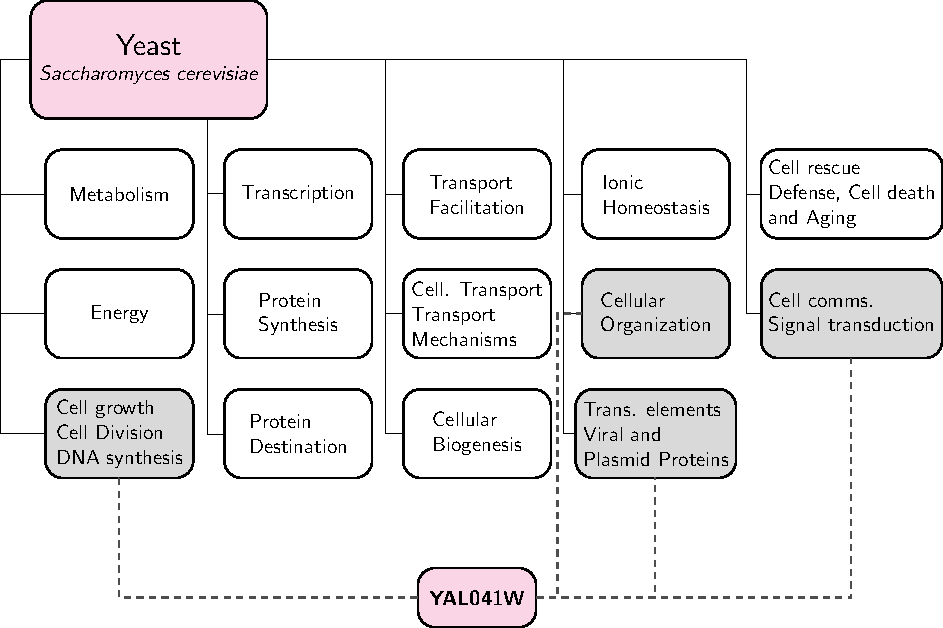
\includegraphics[width=0.75\textwidth]{ch01/demo_ontology}
  \caption{Functional categories of protein YAL041W in \textit{S. cerevisiae}}
  \label{demo:yeast_go}
\end{figure}

\noindent The protein above is associated with multiple functional
categories: cell growth, organization, communication, and viral detection. To
an extent, these categories are not necessarily related to one another yet
they are all performed by a single protein.

\par We define a set of protein functions (or \textit{labels}) as a binary
matrix $\mathbf{Y}$ where each row $i=1 \dots N$ is a protein sample, and
each column $j=1 \dots q$ is a protein function (designated as $\lambda$).
The size of $q$ depends on the number of possible labels in the dataset. In
addition, a protein labelset (a row vector) $\mathbf{y}_n$ is encoded as a
one-hot vector of size $q$. Say we're given a dataset with five functional
categories, $q=5$, and a protein sample $n$ with functions
$\lambda_1, \lambda_4,$ and $\lambda_5$; we then express its labelset as:

\[
    \mathbf{y}_n = \left[\begin{matrix}
        1 & 0 & 0 & 1 & 1
    \end{matrix} \right]
\]

\noindent Here, each index indicates a protein's functional category. More formally, we
represent all protein labels as $\mathbf{Y} \in \{0,1\}^{N \times q}$, where each
row-vector $\mathbf{y}_n \in \{0,1\}^q$ is a labelset containing $q$ labels
$\lambda$.


\newpage
Together, we have the following definition:

\begin{definition}{}
A protein dataset $\mathcal{D}$ consists of $N$ pairs of feature and label
vectors $\{(\mathbf{x}_i, \mathbf{y}_i)\}_{i=1}^{N}$ where $\mathbf{x}_i \in
\mathbb{R}^d$ and $\mathbf{y}_i \in \{0,1\}^q$. In matrix-form, $\mathcal{D}$
consists of feature and label matrices, $\mathcal{D} = \langle \mathbf{X},
\mathbf{Y} \rangle$ where $\mathbf{X} \in \mathbb{R}^{N \times d}$ and
$\mathbf{Y} \in \{0,1\}^{N \times q}$.
\end{definition}

\par We will use this definition as we formulate the protein function
prediction problem as a multilabel classification task.


\section[Protein Function Prediction as a Multilabel Classification Task]
{Protein Function Prediction as a Multilabel\\Classification  (MLC) Task}
\label{MultilabelClassification}

\par Classification is one of the most common tasks in machine learning
(\cite{herrera2016multilabel}). Given input features $\mathbf{X}$ and its
corresponding label $y$, the goal is to find a mapping function $\mathcal{H}:
\mathbf{X} \rightarrow y$ that can accurately associate each set of
attributes to its particular label. For prediction, we formulate the mapping
function as $\mathcal{H}: \mathbf{X} \rightarrow \widehat{y}$. A good example
is image classification: given an image, we train a classifier to distinguish
what particular object it belongs to.

\begin{figure}[!h]
  \centering
  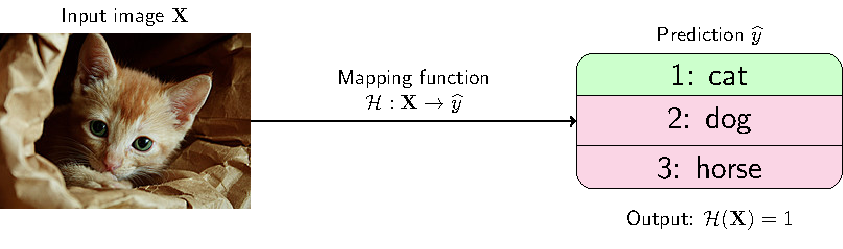
\includegraphics[width=0.70\textwidth]{ch01/demo_tradclass}
  \caption[Demonstration of traditional classification in images]
  {Demonstration of traditional classification in images.\\Cat photo
  from ImageNet (\cite{russakovsky2015imagenet})}
  \label{demo:traditional}
\end{figure}

\par However, proteins can perform multiple functions at once, and the
traditional definition of classification does not apply to the given task.
Instead, the goal now is to discriminate between \textit{multiple labels} and
associate them to the feature set. An apt counterpart to image classification
is scene classification (\cite{boutell2004learning}), where multiple objects
are associated to a given image.

\begin{figure}[!h]
  \centering
  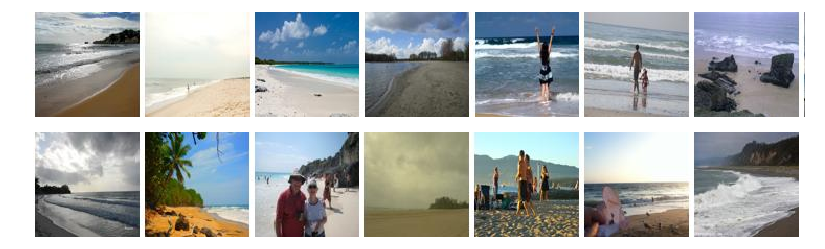
\includegraphics[width=0.95\textwidth]{ch01/demo_multilabel}
  \caption[Demonstration of multilabel classification]
  {Demonstration of multilabel classification.\\Beach photo
  from ImageNet (\cite{russakovsky2015imagenet})}
  \label{demo:multilabel}
\end{figure}

\newpage
\par Protein function prediction behaves similarly to scene classification:
given a protein sample (i.e., the image/scene), find the functional categories
associated with it (i.e., the objects in the scene).  This task is known as
\textit{multilabel classification} (MLC). Notice that in MLC, there are only
two classes for each label $\lambda$: $0$ (does not belong to $\lambda$) and
$1$ (belongs to $\lambda$). Thus, MLC is akin to doing binary classification
for each label. Formally, we define the multilabel classification task as:

\begin{definition}{}
Given a dataset $\mathcal{D}$, find a function $\mathcal{H}$ that maps the
feature matrix $\mathbf{X}$ to a set of labels $\mathbf{Y}$, i.e.,
$\mathcal{H}: \mathbf{X} \rightarrow \mathbf{Y}$. For any unseen instance
$\mathbf{x} \in \mathcal{X}$, where $\mathcal{X} \in \mathbb{R}^d$, we
predict its corresponding label vector $\mathbf{\widehat{y}}$ via
$\mathcal{H}(\mathbf{X}) \subseteq \mathcal{Y}$ where $\mathcal{Y} = \{y_1,
y_2, \dots, y_n, \dots, y_q\}$ and $y_n \in \{0,1\}$\footnote{Adapted from
\cite{zhang2014review}}.
\end{definition}

\par Next, we will discuss a commonly-used approach in solving multilabel
classification problems: binary relevance.

\subsection{Binary relevance in multilabel classification}

\par Binary relevance (BR) decomposes a multilabel problem into a series of
single-label classification tasks (\cite{godbole2004discriminative,
tsoumakas2007multilabel}). The concept is to take any ``off-the-shelf''
classifier $h$ and train it on each label $\lambda$, fitting a total of $q$
classifiers as seen in Figure \ref{demo:binaryrelevance}. Further
modifications to BR include combining labels, or building chains of
classifiers (\cite{read2009classifier}). However, due to BR's conceptual
simplicity and time-complexity\footnote[2]{
    Most problem-transformation techniques have an overhead time-complexity
    depending on the classifier $h$. For Binary relevance, we have $\bigO(q
    \cdot h(N, d))$. At inference, the complexity is $\bigO(q
    \cdot h(d))$. This is relatively faster compared to Classifier Chains
    $\bigO(q \cdot h(N, d + q))$ or Label Ranking $\bigO(q^{2} \cdot h(N, d))$
    (\cite{zhang2014review}).
}, it has been widely used in literature (\cite{zhang2017binary}).

\begin{figure}[!h]
  \centering
  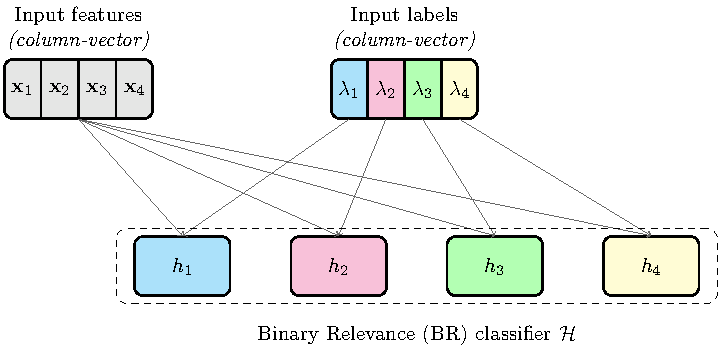
\includegraphics[width=0.65\textwidth]{ch01/demo_binaryrelevance}
  \caption[Binary relevance classification diagram]
  {Binary relevance classification diagram.\\Train $q$ classifiers $h$ for each
  label $\lambda$}
  \label{demo:binaryrelevance}
\end{figure}

\par BR falls under one of the two main approaches in classifying multilabel data:
problem transformation and algorithm adaptation. The former, where BR
belongs, transforms a multilabel problem into separate single-label binary
classification tasks while the latter adapts a classifier to directly handle
multilabel data (\cite{tsoumakas2007multilabel}).

\par We focus on BR because it is easier to treat the classifier as a separate
module from the feature extractor; it is also a simple yet effective method
for multilabel classification (\cite{luaces2012binary}). With BR, a
classifier can be decoupled from a feature extractor, enabling the former to
be tested on variants of the latter. Another reason is that the literature on
problem transformation techniques is extensive enough to enable benchmarking
on different multilabel classifiers in the future (\cite{zhang2014review,
madjarov2012extensive}).

\par This research will concentrate on finding good representations for the BR
classifier to solve the problem of protein function prediction. The process of
obtaining new features from raw data is called \textit{feature extraction}, and
is one of the core ideas in this work. Even if a BR classifier can stand on its
own, we hypothesize that higher performance can be achieved when using the
extracted features rather than the raw attributes themselves.

\section{Extracting Features for Better Data Representation}
\label{FeatureExtraction}

\par One of the core ideas in this work is feature extraction\footnote{
  Feature extraction has been referred to in various ways in literature:
  feature learning, representation learning, manifold learning, etc. We will
  use the term ``feature extraction'' in this work.
}\textemdash where new features are derived from raw attributes for better
data representation, and consequently, better classification. The success of
machine learning algorithms depends on data representations, for it can
entangle manifolds or explanatory factors of variation behind the data
(\cite{bengio2013representation}). 

\par More formally, the goal is to learn a mapping $\phi$ such that $\phi:
\mathbf{X} \rightarrow \mathbf{X}^{\prime}$, where $\mathbf{X}^{\prime}$
represents the extracted features useful\footnote{
  We will preemptively state that ensuring a feature set is useful will
  be the prime motivation of this work. We will attempt to define ``usefulness''
  or \textit{relevance} in Sec. \ref{Motivation}
} to a classifier $\mathcal{H}$. We
hypothesize that using $\mathbf{X}^{\prime}$ should classify better (measured
in accuracy, F-score, etc.) than just using the raw attributes $\mathbf{X}$.
The proceeding section illustrates this idea using the XOR gate.

\subsection{A simple demonstration using the XOR gate}

\par The need for feature extraction is best demonstrated by the XOR problem.
Given two binary inputs, the goal is to separate binary 0's and 1's of the gate
output. We take two inputs $\mathbf{x} = \langle x_{1}$, $x_{2} \rangle, x_1,
x_2 \in \{0,1\}$ as features and the output $y_{i} \in \{0,1\}$ as the label.
With four samples representing all possible bitwise-combinations, a dataset
$\mathcal{D}=\{(\mathbf{x}_{i}, y_{i})\}_{i=1}^{4}$ can be constructed as:

\[
    \mathcal{D} = \{(0,0,0), (0,1,1), (1,0,1), (1,1,0)\}
\]

Assuming we only have access to a linear classifier, the feature-space shown in
Figure \ref{demo:xor} (\textit{left}) proves that classification is difficult
due to linear inseparability\textemdash that is, drawing a single line to
perfectly separate the X's and O's is impossible.  However, if a new
feature-space $\mathbf{x}^{\prime}$ is engineered in such a way that
$\mathbf{x}^{\prime} = \langle {x}^{\prime}_{1}, {x}^{\prime}_2 \rangle$ where
$x^{\prime}_{1} = \text{AND}(\bar{x}_{1}, x_{2})$ and $x^{\prime}_{2} =
\text{AND}(x_{1}, \bar{x}_{2})$, then it is possible to transform $\mathcal{D}$
into dataset $\mathcal{D}^{\prime}=\{(\mathbf{x}^{\prime}_{i},
y_{i})\}_{i=1}^{4}$ such that:

\[
    \mathcal{D}^{\prime} = \{(0,0,0), (1,0,1), (0,1,1), (0,0,0)\}
\]

\par From Figure \ref{demo:xor} (\textit{right}), we can see that
$\mathcal{D}^{\prime}$ is now a linearly separable problem. In this
demonstration, it is evident that hand-engineering features, or
\textit{extracting new features} has been helpful. However, with large
datasets, it will be tedious to manually find useful representations from data.
It is much preferable to automate the whole process. In the next section, we
will turn our attention to an effective way of learning $\phi$ in a
parameterized fashion\textemdash the autoencoder neural network.

\begin{figure}[!t]
  \centering
  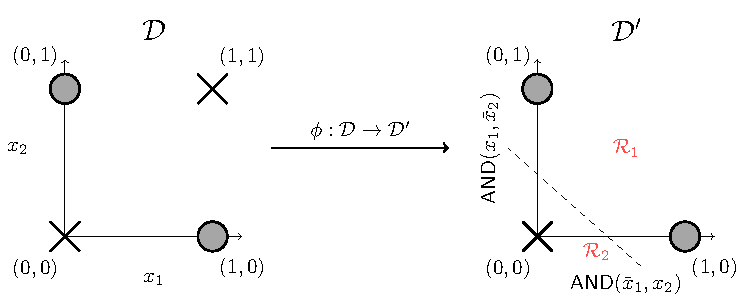
\includegraphics[width=0.75\textwidth]{ch01/demo_xor}
  \caption[Illustration of feature extraction using the XOR gate]
    {Illustration of feature extraction using the XOR gate.\\ Binary `1's are
    represented as circles while binary `0's as cross-marks.}
  \label{demo:xor}
\end{figure}

\subsection{The autoencoder neural network}

\begin{wrapfigure}{r}{0.5\textwidth}
  \centering
  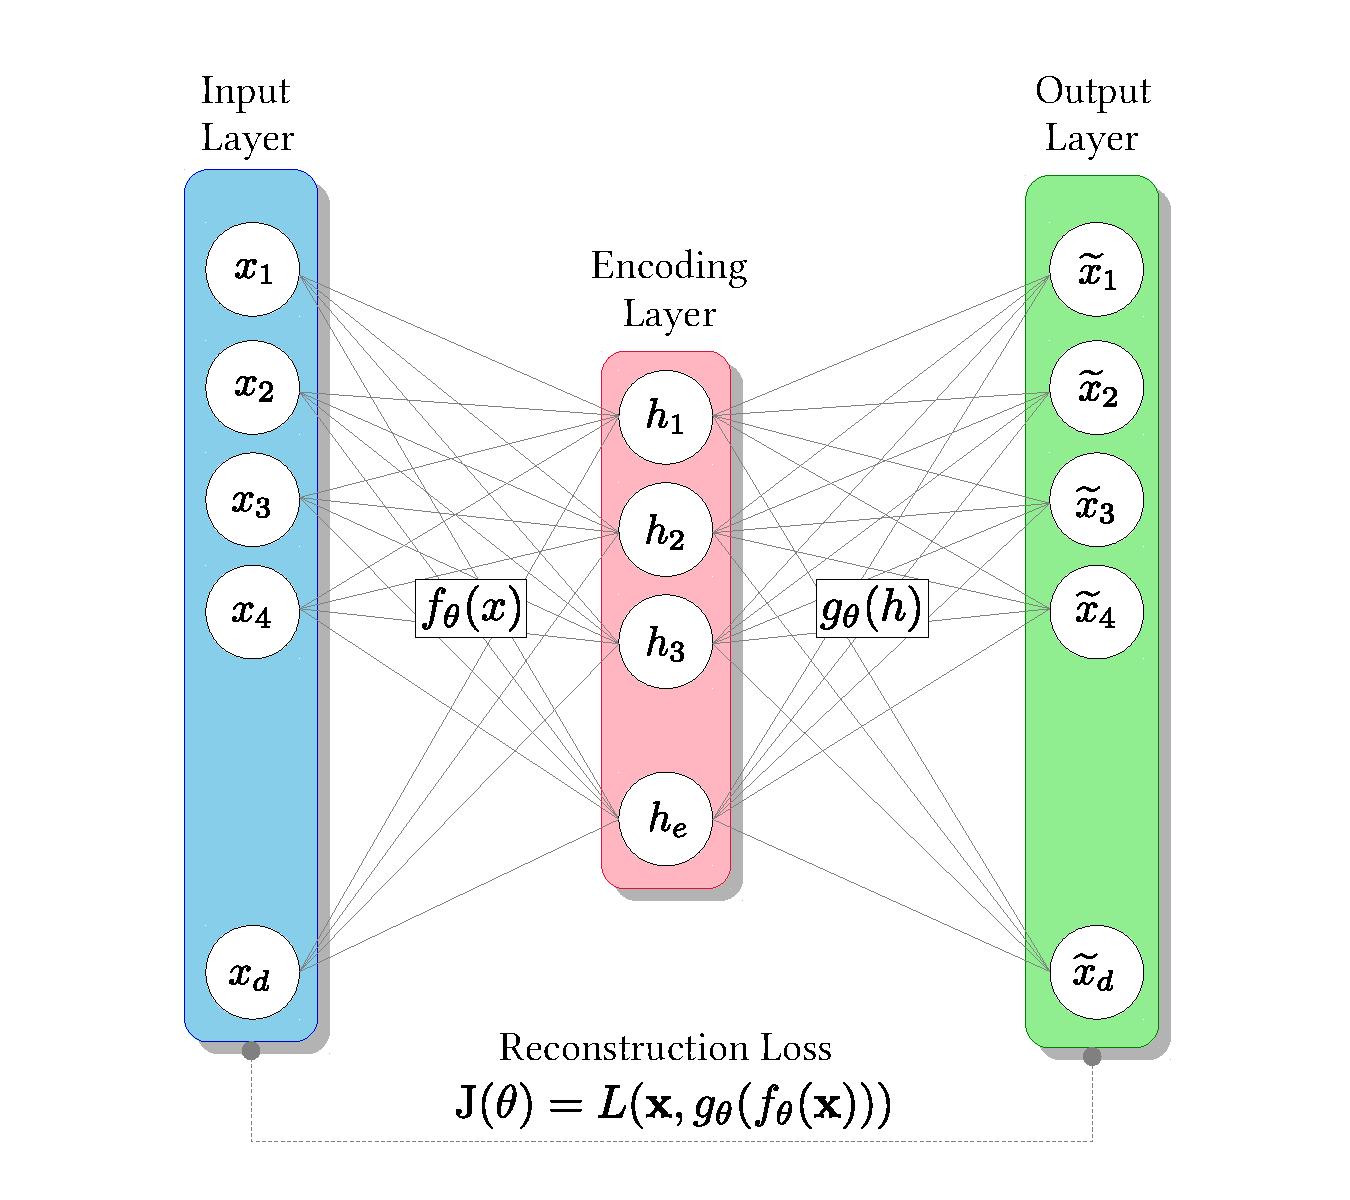
\includegraphics[width=0.40\textwidth]{ch01/schema_autoencoder}
  \caption[Diagram of the basic autoencoder]{
      Diagram of the basic autoencoder
  }
  \label{schema:autoencoder}
\end{wrapfigure}

\par The autoencoder neural network serves as the main framework in our
proposed models.  It was first introduced by \cite{lecun1987phd} and
was subsequently studied by other researchers in the following years
(\cite{bourlard1988auto, hinton1994autoencoders}). The idea is simple yet
powerful: train a network to reconstruct a given input with the
presence of information bottlenecks.

\par Constraining information and reconstructing it are the two key aspects in
training autoencoders. If an autoencoder can reconstruct information
accurately, even with constraints involved, then it has learned the latent
structure of the raw data. The simplest way to constrain an autoencoder is to
introduce architecture bottlenecks: we can limit the number of hidden nodes
less than the feature's original dimension ($e<d$). For a dataset with
$d=100$ dimensions, if we set $e=20$, and the autoencoder was still able to
reconstruct the original data, then it has learned a hidden structure expressed
in a lesser capacity.

\par In practice, an autoencoder's architecture consists of an encoder-decoder
scheme. The encoder function $f_{\theta}$ transforms the original input
$\mathbf{X}$ into a certain representation $\mathbf{h}$ (from $100$ features to
$20$), and the decoder function $g_{\theta^{\prime}}$ converts $\mathbf{h}$
into an approximation of the raw features $\mathbf{\widehat{X}}$ (where
$\mathbf{\widehat{X}} = g_{\theta^{\prime}}(\mathbf{h}) \approx \mathbf{X}$).
By formulating the loss function as a comparison of the original input and its
approximation, we  contrive the network to reconstruct $\mathbf{X}$:

\[
    J(\theta) = L(\mathbf{X}, \mathbf{\widehat{X}}) \quad \text{where} \quad
    \mathbf{\widehat{X}} = (g_{\theta^{\prime}} \circ f_{\theta}) (\mathbf{X})
\]

Algorithm \ref{algo:autoenc} describes the procedure for training an autoencoder.

%=============================================================================
% algo_autoenc.tex
% Copyright (c) 2018. Lester James V. Miranda
%
% This file is part of thesis-manuscript.
%
% thesis-mansucript is free software: you can redistribute it and/or modify
% it under the terms of the GNU General Public License as published by
% the Free Software Foundation, either version 3 of the License, or
% (at your option) any later version.
%
% thesis-manuscript is distributed in the hope that it will be useful,
% but WITHOUT ANY WARRANTY; without even the implied warranty of
% MERCHANTABILITY or FITNESS FOR A PARTICULAR PURPOSE.  See the
% GNU General Public License for more details.
%
% You should have received a copy of the GNU General Public License
% along with thesis-manuscript.  If not, see <http://www.gnu.org/licenses/>.
%
% Created by: Lester James V. Miranda <ljvmiranda@gmail.com>
%=============================================================================

\begin{algorithm}
    \caption{Training an autoencoder neural network}
    \label{algo:autoenc}
    \begin{algorithmic}[1]
    
    \INPUT Raw attributes $\mathbf{X}$
    \OUTPUT Learned parameters $\theta^{\ast}$

    \item[]
    \For{\textit{NumEpochs}}
        \State $\mathbf{h} \gets f_{\theta}(\mathbf{X}) = \sigma(\theta\mathbf{X}^{T} + \theta_0)$
        \Comment Encoder function
        \State $\mathbf{\widehat{X}} \gets g_{\theta^{\prime}}(\mathbf{h}) = \sigma(\theta^{\prime} \mathbf{h}^{T} + \theta^{\prime}_{0})$
        \Comment Decoder with tied-weights, $\theta^{\prime}=\theta^{T}$
        \State $J(\theta) \gets L(\mathbf{X}, \mathbf{\widehat{X}})$
        \Comment Compute loss
        \State \Call{Backpropagation}{$J(\theta)$}
        \Comment Optimize parameters
    \EndFor
    \State \Return $\theta^{\ast}$
    \Comment Return learned parameters
    \end{algorithmic}
\end{algorithm}

The learned parameters $\theta^{\ast}$ encapsulates the latent structure
discovered by the autoencoder. These parameters transform the original data
via the encoder function\textemdash i.e, $ \mathbf{X}^{\prime} =
f_{\theta^{\ast}}(\mathbf{X})$, $f_{\theta^{\ast}} \equiv \phi$\textemdash
and feed the transformation $\mathbf{X}^{\prime}$ into the multilabel
classifier $\mathcal{H}$. Figure \ref{schema:pipeline} illustrates this
simple model. In the next section, we will trace major developments in
machine learning that attempted to solve the protein function prediction
problem while adhering to the framework above.


\begin{figure}[!t]
  \centering
  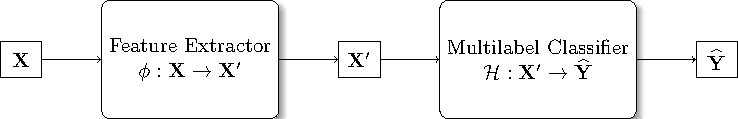
\includegraphics[width=0.85\textwidth]{ch01/schema_pipeline}
  \caption{Simple diagram of the protein function prediction model}
  \label{schema:pipeline}
\end{figure}

\section{Review of Related Literature}
\label{LiteratureReview}

\par There are three major movements we should consider when tracing the
developments of protein function prediction (PFP) in machine learning: first is
(1) direct classification, then by (2) dimensionality reduction, and lastly via
(3) deep feature extraction. Before, machine learning techniques involved
feeding raw data into a classifier, then found the need to reduce the number of
features in the dataset. Later on, ML showed promise by learning suitable data
representations for the classifier. This research falls into the third
category: utilizing deep neural networks to learn representations for
classification. But before that, let's start from the beginning, where raw
protein data is being fed directly to a multilabel classifier.

\paragraph{Direct multilabel classification}
The earliest attempt to solve the protein function prediction problem was
done by \cite{elisseeff2001kernel}. They formulated PFP as a ranking problem
(not yet as a multilabel problem but rather an extension of multiclass
classification), and implemented a variant of the support-vector machine
(SVM) known as Rank-SVM. They tested their technique on \textit{S.
cerevisiae}, giving rise to the now known Yeast dataset. Later on,
\cite{diplaris2005protein} benchmarked various techniques on their own
protein data\textemdash the Genbase dataset. It is noteworthy that in the
conclusion of their work, they expressed their intention to investigate
``alternative representations of the learning problem,'' which brought a slew
of techniques for multilabel classification.

\par This brought forth the main baseline for multilabel classification, the
Binary Relevance (BR) algorithm
(\cite{godbole2004discriminative,tsoumakas2007multilabel}). These were then
extended into Label Powerset (LP) and Classifier Chains (CC)
(\cite{read2009classifier}), but BR's conceptual ease and ``relative speed''
made it stay. Furthermore, various literature reviews attested BR's
performance, especially when paired with an SVM classifier
(\cite{luaces2012binary, zhang2014review,tsoumakas2017data}). For our
research, we will use the Binary Relevance with SVM (BR-SVM) as the baseline
of our work.

\paragraph{Reducing protein data dimensionality} Although binary relevance
has achieved good traction in protein function prediction, training a
classifier for each label can be time-consuming. Researchers have then
resorted to reduce the number of features in protein samples\footnote{The Genbase
dataset, for instance, has $1186$ attributes} using dimensionality-reduction
techniques (\cite{wang2009using, wang2013protein, wang2017protein}); they may
not reduce the number of labels to train their classifier upon, but they can
reduce the time it takes to train one. It is important to note that these
techniques gave a semblance of feature extraction: reducing dimensions in
data may be akin to finding a different representation of a feature space.
However, dimensionality-reduction is still limited primarily due to it being
linear (\cite{cunningham2015linear}). Later on, we will
compare against the work of \cite{wang2013protein} that uses Principal
Component Analysis (PCA) as a dimensionality-reduction technique to a
k-nearest neighbors classifier (k-NN). They were able to reduce a protein
dataset with $353$ features into $204$, achieving good classification
performance. We chose this method because it follows a similar pipeline to
Figure \ref{schema:pipeline}, and uses a similar data source (gene
expressions) to our protein benchmark.

\paragraph{Deep feature extraction in protein function prediction}
Reducing dimensions in protein data has sped-up and improved classification,
but common approaches such as principal component analysis (PCA) are linear
(\cite{bengio2013representation}), failing to capture the nonlinearities
present in a protein's feature space. This gave way for researchers to apply
deep learning techniques to protein data\textemdash both for protein
sequences (\cite{bhola2014machine,kulmanov2017deepgo, zou2017protein}) and
expressions (\cite{baldi2001bioinformatics, chicco2014deep}). We
will benchmark against \cite{chicco2014deep}, who used a deep autoencoder
network to extract features from protein gene expressions. Comparing against
this method enables us to have a baseline, traditional autoencoder
implementation to check our proposed architecture upon.

\par As mentioned, our work falls under the last category of deep feature
extraction. One major advantage of this technique is that it can provide a
more separable feature space as demonstrated earlier by the XOR example. In
addition, we can decouple the feature extractor from the classifier with
binary relevance, enabling us to test on different variants of the
classifier. However, we argue that extracting features is not enough. It is
important to learn representations relevant with respect to the classifier.
The next section elaborates this work's motivation\textemdash clarifying the
meaning of feature relevance\textemdash and formulate the problem and
research hypothesis throughout this work.

\section{Research Motivation}
\label{Motivation}

\par Learning new representations from raw protein data has been effective in
capturing nonlinearities in the feature space\textemdash a feat unachievable
by dimensionality reduction or direct classification alone. However, there is
a need to ensure that the extracted features are indeed \textit{relevant}. It
is important to have useful representations, not just linear combination of
features and weights optimizing a loss function. Given these, we state our
reseasrch motivation:

% State the motivation of this work: it's not enough to extract features
% it is also important to extract relevant features.
\begin{quote}
  \itshape
  \small
  Although feature learning in protein data has been effective, we posit that
  merely extracting features is not enough. It is important to ensure that
  the extracted features are relevant with respect to the task at hand.
  Hence, we propose two autoencoder-based techniques to accomplish this task.
  Extracting relevant features should improve a classifier's predictive
  performance, bringing us a step closer to a faster and more efficient
  annotation of protein functions.
\end{quote}

\paragraph{Definitions of relevance}
Relevance depends on the question: ``relevant to what?''. According to
\cite{blum1997selection}, features must be relevant with respect to:
\begin{itemize}
  \item the target concept (i.e. protein functions), and
  \item the task at hand (i.e., multilabel classification)
\end{itemize}

\par Various definitions of feature relevance exist depending on the
problem's goal. Because our main task is classification, we will adhere to
the definition of relevance as ``incrementally useful'':

\begin{definition}
  \label{DefRelevance}
   Given a dataset $\mathcal{D}$, a learning algorithm $\mathcal{H}$ and a
   feature set $\mathbf{X}$. A feature set $\mathbf{X}^{\prime}$ is
   incrementally useful to $\mathcal{H}$ with respect to $\mathbf{X}$ if the
   accuracy of the hypothesis that $\mathcal{L}$ produces using
   $\mathbf{X}^{\prime}$\footnote{Adapted from \cite{blum1997selection}}
   is better than the accuracy achieved using just the
   feature set $\mathbf{X}$.
\end{definition}

\par\noindent For multilabel classification, we will be using a different set
of metrics instead of accuracy. Originally, \cite{blum1997selection} refers to
a subset of the raw features $\{x_{i}\} \cup \mathbf{X}$, but they went at
length extending this definition to linear combinations of features, rather
than just relevant individual features. This validates the assumption that
relevant features should produce better predictions. In the next section, we
will formulate the problem and state our research hypothesis.

\subsection{Problem formulation and hypothesis}

\par The goal of this work is to extract a set of relevant features to
improve a classifier's performance in predicting protein functions. Formally,
the problem is defined as:

\begin{definition}
  \label{DefProblem}
  Given a dataset $\mathcal{D}=\langle \mathbf{X}, \mathbf{Y} \rangle$ and a
  classifier $\mathcal{H}$, construct a feature extractor $\phi$ that learns
  a feature set $\mathbf{X}^{\prime}$ by $\phi: \mathbf{X} \rightarrow
  \mathbf{X}^{\prime}$ such that $\mathbf{X}^{\prime}$ is relevant with respect
  to $\mathcal{H}$ and $\mathbf{X}$ by virtue of Def. \ref{DefRelevance}.
\end{definition}

\par\noindent We will present two autoencoder-based models to accomplish this
task.  Because these models extract task-relevant features, we expect that
classifier performance will improve. More formally, we state our research
hypothesis as:

\begin{definition}
  \label{DefHypothesis}
  If a feature extractor $\phi$ extracts task-relevant features
  $\mathbf{X}^{\prime\ast}$ for a multilabel classifier $\mathcal{H}$, then
  the performance of $\mathcal{H}(\mathbf{X}^{\prime\ast})$ should be
  better than the same classifier but with raw attributes $\mathbf{X}$
  or a non-relevant feature set $\mathbf{X}^{\prime}$.
\end{definition}


\par The next chapter (Ch. \ref{SDAEChapter}) will discuss the Stacked
Denoising Autoencoder (SdAE), examining its denoising capability to obtain
relevant features from an inherently noisy protein dataset. SdAEs were
originally used in image denoising, yet this work will explore its efficacy
in protein datasets in a multilabel setting. The following chapter (Ch.
\ref{SelectiveChapter}) will improve upon the autoencoder architecture via a
Mutually-Competitive autoencoder that learns a sparse and relevant feature
set by means of mutual competition. All resulting features from these models
will then be fed into a BR-SVM classifier. These autoencoder-based methods
will be tested with respect our hypothesis stated in Definition
\ref{DefHypothesis}.

%=============================================================================
% Denoising Chapter
% Copyright (c) 2018. Lester James V. Miranda
%
% This file is part of thesis-manuscript.
%
% thesis-manuscript is free software: you can redistribute it and/or modify
% it under the terms of the GNU General Public License as published by
% the Free Software Foundation, either version 3 of the License, or
% (at your option) any later version.
%
% thesis-manuscript is distributed in the hope that it will be useful,
% but WITHOUT ANY WARRANTY; without even the implied warranty of
% MERCHANTABILITY or FITNESS FOR A PARTICULAR PURPOSE.  See the
% GNU General Public License for more details.
%
% You should have received a copy of the GNU General Public License
% along with thesis-manuscript.  If not, see <http://www.gnu.org/licenses/>.
%
% Created by: Lester James V. Miranda <ljvmiranda@gmail.com>
%=============================================================================

\chapter[Stacked Denoising Autoencoder for Protein Function Prediction]{
    \huge
    Feature Extraction using a Stacked Denoising Autoencoder for Protein
    Function Prediction
}
\label{SDAEChapter}

\par In this chapter, we will discuss our preliminary work where we extracted
robust features using a stacked denoising autoencoder (SdAE). This work's main
contribution is the successful domain-transfer of SdAE, commonly-used in
images, in multilabel protein data. We start by describing the SdAE
architecture (Sec. \ref{SDArchitecture}), then illustrate how it fits in the
protein function prediction pipeline (Sec.  \ref{SDPipeline}). Then, we
describe our experimental set-up (Sec.  \ref{SDSetup}), present our findings
(Sec. \ref{SDResults}), and draw conclusions (Sec. \ref{SDConclusions}).

\section{Stacked Denoising Autoencoder}
\label{SDArchitecture}

\begin{wrapfigure}{r}{0.53\textwidth}
  \centering
  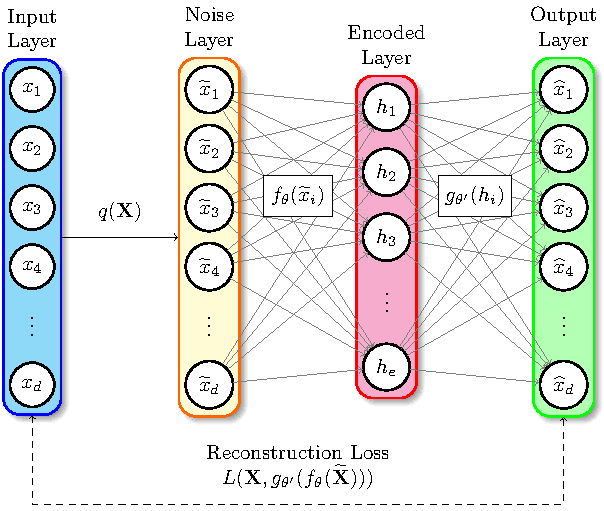
\includegraphics[width=0.5\textwidth]{ch03/sdae}
  \caption{Stacked denoising autoencoder}
  \label{schema:sdae}
\end{wrapfigure}

\par A stacked denoising autoencoder (SdAE) is a type of autoencoder that
corrupts the input data before reconstruction (\cite{vincent2010stacked}). It
is an extension of denoising autoencoders where layers are stacked and
greedily-trained\footnote{Greedy layer-wise training were once implemented
for practicality and to conserve memory (\cite{bengio2007greedy}). Today,
deep autoencoders like SdAE are trained end-to-end.}
(\cite{vincent2008denoising}).

\par Figure \ref{schema:sdae} illustrates the SdAE architecture. Given an
input data $\mathbf{X}$, we apply a corrupting function
$q(\mathcal{X}=\mathbf{X})$ to obtain a set of \textit{corrupted inputs}
$\mathbf{\widetilde{X}}$. We use the corrupted input to train the
autoencoder, but we compute the reconstruction loss by comparing the
reconstructed features $\mathbf{\widehat{X}}$ with the original data
$\mathbf{X}$. By learning from a set of corrupted inputs, we can capture the
``main factors of variations in the data (\cite{vincent2008denoising}),''
enabling our model to generalize unseen instances in the problem domain.
In theory, this should improve classification performance.

\subsection{Generalization and manifold learning}

\begin{wrapfigure}{r}{0.5\textwidth}
  \centering
  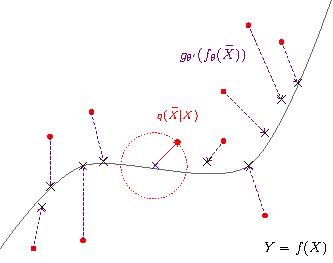
\includegraphics[width=0.45\textwidth]{ch03/demo_manifold}
  \caption[Manifold demonstration in SdAE]{Manifold learning in SdAE. Adapted
  from \cite{vincent2008denoising}}
  \label{demo:manifold}
\end{wrapfigure}

\par We'll spend some time examining how a stacked denoising autoencoder's
corrupting function enables the model to generalize during training.
Generalization prevents model overfitting, i.e. fitting too close to the
training set resulting to poor performance on the test set. The test set
represents unseen or future instances where we want to perform well.  Thus, our
goal is to obtain the main factors of variation from the samples.  Perceiving
SdAEs this way permits us to transfer this method to a different
domain\textemdash in our case, multilabel protein data\textemdash with more
confidence.

\par Say we're given a training dataset $X$ (marked by $\times$) that lies on
a manifold represented by the spline in Figure \ref{demo:manifold}. In
practice, we don't know what the spline looks like and the training data is
not always perfect.\footnote{
  The training data will not always be lying on-top of the spline. We know
  this to be true because there will always be unmodeled physics or
  measurement errors (i.e., $x+\epsilon$) that we cannot always account
  during data acquisition.
} Our task is to learn the manifold equivalent to identifying the structure
of the spline. Applying the noise function $q(\widetilde{X}|X)$ results to
data points $\widetilde{x}$ (red dots) that are further away from the spline.
SdAE learns the manifold by projecting the noisy inputs back as demonstrated
by the dotted lines $g_{\theta^{\prime}}(f_{\theta}(\widetilde{X}))$
(\cite{vincent2008denoising}). As shown, the projections can approximate the
manifold and accommodate subtle variations even if a new data point is
slightly-off the spline. This idea is crucial given the pretext that protein
datasets are inherently noisy due to unaccounted measurement errors (Sec.
\ref{ProteinFunctionPrediction}).

\begin{figure}[h]
  \centering
  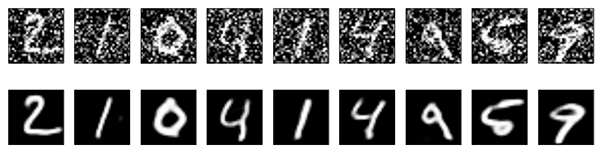
\includegraphics[width=0.9\textwidth]{ch03/demo_denoise}
  \caption[Demonstration of image denoising via SdAE]{
    Demonstration of image denoising via SdAE (\cite{chollet2016autoencoders})}
  \label{demo:denoise}
\end{figure}

\par Figure \ref{demo:denoise} demonstrates the reconstruction capability of
SdAE in the MNIST dataset. It has learned to ``ignore'' the unnecessary
variations in the data (noise) while focusing on the structural manifold of
the image. As a result, it was able to reproduce cleaner images from noisy
samples. It is evident that SdAE has learned to distinguish between relevant
and irrelevant aspects of the image: it retained useful information (the
actual digit) while discarding unnecessary ones (random noise).

\subsection{Practical considerations for SdAE training}

\par Table \ref{exp:noise_types} describes three different corrupting functions
for SdAE. In our model, we used the salt and pepper noise (SP); this choice is
motivated by our preprocessing step where we normalized the inputs into the
range $\left[0,1\right]$. It is also a natural choice due to the squashing
effect caused by the sigmoid activation function during training. 

\begin{table}[!h]
  \centering
  \caption[Different types of corrupting functions $q(\mathcal{X})$ for SdAE]
  {Different types of corrupting functions $q(\mathcal{X})$ for SdAE\\
  (\cite{vincent2010stacked})}
  \label{exp:noise_types}
  \begin{tabular}{@{}rp{0.70\textwidth}@{}}
      \toprule
      Noise            & Description                                                   \\ \midrule
      Gaussian         & additive isotropic Gaussian noise $\mathbf{\widetilde{x}} |
                         \mathbf{x} \sim \mathcal{N}(\mathbf{x}, \sigma^2 I)$          \\
      Masking          & a random sample of elements in $\mathbf{x}$ are forced to $0$ \\
      Salt-and-Pepper  & a random sample of elements in $\mathbf{x}$ is set to their
                         maximum or minimum value (usually $0$ or $1$)                 \\\bottomrule
  \end{tabular}
\end{table}

\par We introduce a hyperparameter, noise rate ($r$), that dictates how much of
the elements in $\mathbf{x}$ will be affected by the noise. For
salt-and-pepper, this determines the percentage of features, that will be set
to $0$ or $1$ based on a coin flip i.e., $P(0) = P(1) = 0.5$.

\par Lastly, Algorithm \ref{algo:sdae} describes the training procedure for
SdAE.  It is similar to a deep autoencoder (Alg. \ref{algo:autoenc}), but the
difference is that we corrupt the inputs first. In the next section, we will
present how we incorporated SdAE in the protein function prediction pipeline.

%=============================================================================
% algo_sdae.tex
% Copyright (c) 2018. Lester James V. Miranda
%
% This file is part of thesis-manuscript.
%
% thesis-mansucript is free software: you can redistribute it and/or modify
% it under the terms of the GNU General Public License as published by
% the Free Software Foundation, either version 3 of the License, or
% (at your option) any later version.
%
% thesis-manuscript is distributed in the hope that it will be useful,
% but WITHOUT ANY WARRANTY; without even the implied warranty of
% MERCHANTABILITY or FITNESS FOR A PARTICULAR PURPOSE.  See the
% GNU General Public License for more details.
%
% You should have received a copy of the GNU General Public License
% along with thesis-manuscript.  If not, see <http://www.gnu.org/licenses/>.
%
% Created by: Lester James V. Miranda <ljvmiranda@gmail.com>
%=============================================================================

\begin{algorithm}
    \caption{Training a stacked denoising autoencoder}
    \label{algo:sdae}
    \begin{algorithmic}[1]
    
    \INPUT Raw attributes $\mathbf{X}$, Noise rate $r$
    \OUTPUT Learned parameters $\theta^{\ast}$

    \item[]
    \State $\mathbf{\widetilde{X}} \gets q(\mathbf{X}, r)$
    \Comment Corrupt inputs
    \For{\textit{NumEpochs}}
        \State $\mathbf{h} \gets f_{\theta}(\mathbf{\widetilde{X}}) = \sigma(\theta\mathbf{\widetilde{X}}^{T} + \theta_0)$
        \Comment Encoder function
        \State $\mathbf{\widehat{X}} \gets g_{\theta^{\prime}}(\mathbf{h}) = \sigma(\theta^{\prime} \mathbf{h}^{T} + \theta^{\prime}_{0})$
        \Comment Decoder with tied-weights, $\theta^{\prime}=\theta^{T}$
        \State $J(\theta) \gets L(\mathbf{X}, \mathbf{\widehat{X}})$
        \Comment Compute loss
        \State \Call{Backpropagation}{$J(\theta)$}
        \Comment Optimize parameters
    \EndFor
    \State \Return $\theta^{\ast}$
    \Comment Return learned parameters
    \end{algorithmic}
\end{algorithm}


\section{Protein Function Prediction Pipeline}
\label{SDPipeline}

\begin{figure}[!t]
  \centering
  \includegraphics[width=0.90\textwidth]{ch03/schema_traintest}
  \caption[Protein function prediction pipeline]{Protein function prediction
  pipeline for the stacked denoising autoencoder}
  \label{schema:traintest_sdae}
\end{figure}

\par The protein function prediction pipeline consists of a (1) \textit{feature
extraction} and (2) \textit{multi-label classification} stage as shown in
Figure \ref{schema:traintest_sdae}.\footnote{
    Except for the corruption part, the pipeline in the mutually-competitive
    autoencoder (Chapter \ref{SelectiveChapter}) looks exactly like this.
} 
This follows the blueprint introduced in Figure \ref{schema:pipeline}: we have
a feature extractor $\phi$ that derives new features $X^{\prime}$ to train a
multilabel classifier $\mathcal{H}$. Here, the SdAE takes the role of the
feature extractor, and a binary-relevance support-vector machine (BR-SVM) as
the classifier. Our main goal is to find the best set of features $X^{\prime}$
that improves $\mathcal{H}$'s predictive performance. As with standard machine
learning practice, we have two phases\footnote{
  We usually split the dataset into training and test data such that
  $\mathcal{D} = \{\mathcal{D}_{tr}, \mathcal{D}_{ts}\}$. We didn't put the
  subscripts $tr$ and $ts$ for it can be easily inferred which set is being
  used in a given context.
}:

\begin{itemize}
  \item \textit{Training phase}: our goal is to learn the parameters $\theta$
  and $W$ for the extractor ($\phi$) and classifier ($\mathcal{H}$) stages
  respectively. We first train the SdAE using Alg. \ref{algo:sdae}, and use
  the learned $\theta^{\ast}$ to encode the training dataset for fitting
  BR-SVM. We use the mean-square error (MSE) as the loss-function for $\phi$ and
  L2-SVM for $\mathcal{H}$:
  \begin{align}
    % Feature Extractor Loss
    \label{eqn:loss_fe_sdae}
    L(\mathbf{X},g_{\theta^{\prime}}(\mathbf{h}^{\prime})) &=
      \dfrac{1}{2}(\mathbf{X} - g_{\theta^{\prime}}(\mathbf{h}^{\prime}))^{2}\\
    % Multilabel classifier loss
    \label{eqn:loss_clf_sdae}
    J(\mathbf{X}^{\prime}, \widehat{\mathbf{Y}}, \mathbf{Y}) &= \sum_{\widehat{\mathbf{y}}_i \neq \mathbf{y}_{i}} \text{max}(0, W^{T}_{\widehat{\mathbf{y}}_{i}} \mathbf{x}_{i}^{\prime} - W^{T}_{\mathbf{y}_i}\mathbf{x}^{\prime}_i + \Delta)^2
  \end{align}
  \item \textit{Test phase}: this phase represents the scenario where we need
  to predict from unseen instances of protein data. We simply take the
  learned parameters $\{\theta^{\ast}, W^{\ast}\}$ and pass the test data
  through the encoder and classifier. The encoder derives new features given the
  equation: 
  \begin{align}
    % Encoder equation
    \label{eqn:encoder_mc_sdae}
    f_{\theta^{\ast}}(\mathbf{X}_{ts}) = \theta^{\ast T} \mathbf{X}_{ts} + \theta_{0}^{\ast}
  \end{align}
 
  \noindent Then the classifier infers from the derived features, producing a set of
  predictions $\mathbf{\widehat{Y}}_{ts}$. We compare our predictions to a
  held-out set of ground-truth labels using the metrics described in the next
  section.
\end{itemize}

\newpage
\subsection{Evaluation metrics}

To evaluate the performance of our prediction model, we will use the following
metrics\footnote[2]{\textit{tp}: true positive, \textit{fp}: false positive,
\textit{tn}: true negative, \textit{fn}: false negative}:

\begin{align}
    \text{Hamming Loss (H)} &= \dfrac{1}{N \cdot L} \sum_{i=1}^{N} \sum_{j=1}^{L}
    \text{XOR}(y_{ij}, \widehat{y}_{ij}) \\
    \text{Precision (P)} &=
    \dfrac{1}{N}\sum_{i=1}^{N}\dfrac{|\mathbf{\widehat{y}}_{i} \cap
    \mathbf{y}_{i}|}{|\mathbf{\widehat{y}_{i}}|} = \dfrac{tp}{tp + fp} \\
    \text{Recall (R)} &=
    \dfrac{1}{N}\sum_{i=1}^{N}\dfrac{|\mathbf{\widehat{y}}_{i} \cup
    \mathbf{y}_{i}|}{|\mathbf{\widehat{y}_{i}}|} = \dfrac{tp}{tp + fn} \\
    \text{F-score (F)} &=
    \dfrac{1}{N}\sum_{i=1}^{N} \dfrac{2 | \mathbf{\widehat{y}}_{i} \cup
        \mathbf{y}_{i}|}{|\mathbf{\widehat{y}}_{i} | + |\mathbf{y}_{i}|} =
        \dfrac{2 (\text{P} \cdot \text{R})}{\text{P} +
        \text{R}}
\end{align}

\par We will also compute for a fifth metric, the Area Under the ROC Curve
(AUROC), to serve as proxy for accuracy. For benchmarking, we will use the AUROC,
Hamming-Loss and F-score. Note that these metrics will exactly be the same for
our work on mutually-competitive autoencoders in Chapter \ref{SelectiveChapter}.

\section{Experimental Set-up}
\label{SDSetup}

\par We performed two (2) sets of experiments for the SdAE-based protein
function prediction pipeline. First, we checked how each hyperparameter,
i.e., noise rate ($r$) and number of encoding units ($e$), affects a
classifier's predictive performance. Then, we benchmarked our model against
different techniques in literature. Table \ref{exp:setup_sdae}
shows a summary of all experiments conducted in this work.

\begin{table}[h]
  \centering
  \caption{Summary of experiments}
  \label{exp:setup_sdae}
  \begin{threeparttable}
      \begin{tabular}{@{}rp{0.65\textwidth}@{}}
          \toprule
          Experiment & Description                                                            \\ \midrule
          \textit{Hyperparameter tests}                                                       \\
          Nb. of encoding units, $e$    & Test overcomplete and undercomplete configurations. \\
          Noise rate, $r$               & Sweep $k$-values in the range $\left[0,1\right]$    \\ \cmidrule{1-2} 
          \textit{Analysis \& benchmark}                                                      \\
          Model quality                 & Plot ROC and PR curves\tnote{1}                     \\
          Benchmark analysis            & Compare SdAE pipeline to other techniques\tnote{2}  \\ \bottomrule
      \end{tabular}
      \begin{tablenotes}
        \footnotesize
        \item[1] ROC - Receiver Operating Characteristic, PR - Precision--Recall
        \item[2] Friedman's test \parencite{friedman1937use} and post-hoc
        Bonferroni-Holm test \parencite{holm1979simple} were employed to
        measure statistical significance as recommended by
        \cite{demsar2006statistical}.
      \end{tablenotes}
    \end{threeparttable}
\end{table}

\par Lastly, Table \ref{exp:implementation_sdae} describes the experimental
environment for running the tests. The neural network was trained on an
NVIDIA Titan X (Pascal) GPU while the classifier was fitted using an Intel
Xeon 2.2GHz CPU. The majority of the code was written in Python 3.6.X using
the \href{https://www.tensorflow.org/}{Tensorflow} and
\href{https://keras.io/}{Keras} package. 

\begin{table}[t]
  \centering
  \caption{Experimental environment}
  \label{exp:implementation_sdae}
  \begin{threeparttable}
  \begin{tabular}{@{}rp{0.70\textwidth}@{}}
      \toprule
      Environment                    & Value                                             \\ \midrule
      \textit{Validation and testing}                                                    \\
      Number of trials               & 10: mean and std. dev. reported                   \\
      Train--validation--test split  & 50--30--20                                        \\ \cmidrule{1-2}
      \textit{Hardware dependencies}                                                     \\
      Number of cores\tnote{1}       & 10 in use (40 maximum)                            \\
      CPU                            & Intel Xeon 2.2GHz: Classifier training            \\
      GPU                            & NVIDIA Titan X (PASCAL): Neural network training  \\ \cmidrule{1-2} 
      \textit{Software dependencies}                                                     \\
      Language                & Python 2.7, 3.6 (compatible to both versions)            \\
      Libraries               & Tensorflow 1.2.1, Keras 2.1.2, Numpy 1.14.2              \\ \bottomrule
  \end{tabular}
  \begin{tablenotes}
    \footnotesize
    \item[1] We implemented a distributed scheme for training the classifier.
    Please see Appendix \ref{AppendixDistributed}.
  \end{tablenotes}
  \end{threeparttable}
\end{table}

\section{Results and Discussion}
\label{SDResults}

In this section, we'll present the results listed in Table
\ref{exp:setup_sdae}. First, we'll look into how different hyperparameter
settings\textemdash namely, noise rate ($r$) and number of encoding units
($e$)\textemdash affect the model as a whole. Then, we'll inspect the quality
of our model, and compare it with various works in literature.  For
implementation details, please see Appendix \ref{AppendixImplementation}.

\subsection{Characterizing the autoencoder model}
\label{SDExperimentsHyperparam}

Our goal in this experiment is to find a pattern governing model behavior
with respect to different hyperparameter values. The idea is to take a
hyperparameter $\mathcal{P}$ and change its value while measuring the Area
under the ROC curve (AUROC). We then plot the results for both train and
validation data. We repeat this experiment for all datasets.

\subsubsection{Experiments on the Yeast Dataset}
\label{SDExperimentsHyperparamYeast}

Figure \ref{results:sdae_char_yeast} shows the characterization results for
Yeast. Recall that validation set performance should always be lower than
training set performance, as the former simulates unseen samples. Here we can
observe the following:

\begin{itemize}
  \item Undercomplete autoencoders perform well without much overfitting.
      Overfitting can be observed with higher values of $e$, exemplified by the
      large gap between training and validation set performance; the model can
      predict the training data well, but fails to accommodate unseen instances
      of the validation data.
  \item Adding noise is beneficial, but too much noise can damage the model.
      Noise provides a good generalization ability to the model, and this
      confirms the ideas presented in denoising autoencoder literature
      (\cite{vincent2008denoising, vincent2010stacked}).
\end{itemize}
 
\begin{figure}[!t]
  \centering
  \begin{subfigure}[b]{0.48\textwidth}
    \includegraphics[width=\textwidth]{ch03/hyperparams_yeast}
    \caption{Yeast}
    \label{results:sdae_char_yeast}
  \end{subfigure}
  \begin{subfigure}[b]{0.48\textwidth}
    \includegraphics[width=\textwidth]{ch03/hyperparams_genbase}
    \caption{Genbase}
    \label{results:sdae_char_genbase}
  \end{subfigure}
  \caption{Model behavior on protein benchmarks}
  \label{results:sdae_char}
\end{figure}

\subsubsection{Experiments on the Genbase Dataset}
\label{SDExperimentsHyperparamGenbase}

Figure \ref{results:sdae_char_genbase} shows the results for Genbase. A similar
procedure was performed for both training and validation data. We can infer
the following from the plots:

\begin{itemize}
  \item SdAE performance on Genbase is good overall. The small gap between
      training and validation performance shows that the model can perform well
      even with unseen instances of the data.
  \item Adding noise is also beneficial, but, similar to Yeast, may lead to
      overfitting if too much. Notice that validation performance is flat, this
      is due to the network having a smaller number of encoding units and
      shorter training time in this set-up ($e=50$ and $\text{epochs}=100$).
\end{itemize}

\subsection{Key results for the stacked denoising autoencoder}

In this section, we present our key results for the stacked denoising
autoencoder. First, we plot model quality in terms of the Receiver Operating
Characteristic (ROC) and Precision-Recall curves, then we present
benchmarking results against different models. Unlike the previous
experiment, we'll be reporting test set performance instead of the validation
set.

\subsubsection{Assessing model quality}

\par The goal of this experiment is to check if the SdAE-based pipeline can
indeed predict protein functions effectively. We can achieve this by plotting
the Receiver Operating Characteristic (ROC) and Precision-Recall (PR) curves
for both datasets and interpreting their shapes. 

\begin{figure}[!h]
  \centering
  \includegraphics[width=0.95\textwidth]{ch03/ql_yeast}
  \includegraphics[width=0.95\textwidth]{ch03/ql_genbase}
  \caption[Receiver Operating Characteristic (ROC) and Precision-Recall (PR)
  curves for the two protein benchmarks]{
    Receiver Operating Characteristic (ROC) and Precision-Recall (PR) curves
    for both Yeast (\textit{top}) and Genbase (\textit{bottom}) datasets.
  }
  \label{results:sdae_quality}
\end{figure}


\par A good indicator of quality for an ROC curve is to check how far the
orange line, representing the FPR and TPR at different cutoff points, is from
the baseline (representing a random classifier). It is apparent that for both
datasets, the curve is way above the baseline\textemdash moreso with
Genbase. In addition, measuring the AUROC gives a good predictive accuracy.
On the other hand, Precision-Recall curves show the tradeoff between
precision and recall for both datasets. It is apparent that Genbase has a
consistently high precision, whereas Yeast has decent quality. In the next
experiment, we'll put our prediction pipeline into context by comparing it
with other works in literature.


\subsubsection{Benchmark analysis}

\par In this experiment, we will compare against various protein function
prediction models in literature. The AUROC, F-score, and Hamming Loss will
measure model performance for both datasets. The results can be seen in
Tables \ref{results:sdae_benchmark_yeast} and
\ref{results:sdae_benchmark_genbase}

\par In addition, we conducted Friedman's test to assess significance in our
measurements. The null hypothesis $H_{0}$ dictates that there is no
significant difference between the groups. The ``Sig.'' column indicates the
extent in $\alpha$ in which we can reject $H_{0}$. The intuition is: the more
stars, the more significant the differences are in the results.

\par For most metrics, the SdAE-based prediction pipeline performs well.
However, it is interesting that PCA (M1) and AE (M2) -based models have a
better AUROC performance. This can be attributed to some models having high
numbers of false negatives in their predictions, resulting to higher
accuracy given sparse labelsets. In fact, it may be easier to get high accuracy
by just predicting all samples as a zero-vector because of label sparsity.
However, if we look into the F-score metric, our model's predictive ability
becomes more apparent. Its high F-score suggests that our prediction pipeline
can better balance between precision and recall (false positives and false
negatives). Lastly, an overall comparison using a post-hoc Bonferroni-Holm test
shows that our SdAE-based model outperforms other models, especially the
baseline. Outperforming the baseline is critical because it validates our claim
that using feature extraction is beneficial to multilabel classification.

\begin{table}[!t]
%
\centering
\begin{threeparttable}
\caption{Benchmark analysis on Yeast dataset}
\label{results:sdae_benchmark_yeast}
%
\begin{tabular}{@{}rr*{5}{l}@{}}
\toprule
        & & \multicolumn{5}{c}{Prediction Model\tnote{1}} \\ \cmidrule{3-6}
Metrics & Avg.      & Baseline       & M1             & M2                 & Proposed\tnote{2} & Sig.\tnote{3}\\
\midrule
AUROC   & micro     & \num{0.667(3)} & \num{0.666(2)} & \num{0.643(1)}     & \hg\num{0.668(4)}  & *** \\
        & macro     & \num{0.655(3)} & \num{0.659(2)} & \hg \num{0.662(1)} & \num{0.648(2)}     & *** \\
        & sample    & \hg\num{0.670(3)} & \num{0.656(2)} & \num{0.643(1)}  & \num{0.657(3)}     & *** \\
F-score & micro     & \num{0.548(4)} & \num{0.538(2)} & \num{0.530(1)}     & \hg\num{0.579(3)}  & *** \\
        & macro     & \num{0.597(4)} & \num{0.603(2)} & \num{0.590(1)}     & \hg\num{0.613(2)}  & *** \\
        & sample    & \num{0.536(3)} & \num{0.524(2)} & \num{0.517(1)}     & \hg\num{0.572(3)}  & *** \\
Hamming Loss & --   & \num{0.322(2)} & \num{0.343(2)} & \num{0.354(1)}     & \hg \num{0.231(3)} & *** \\
\bottomrule
\end{tabular}
%
\begin{tablenotes}
        \footnotesize
    \item[1] M1: \cite{wang2013protein}, M2: \cite{chicco2014deep}
    \item[2] Feature ext.: $\{r=0.75,e=103-100-80\}$, BR-SVM: $\{C=\num{1.00}, \gamma=\num{1.292e-2}\}$
    \item[3] Significance: *-$p\leq 0.1$, **-$p\leq 0.05$, ***-$p\leq 0.01$
\end{tablenotes}
%
\end{threeparttable}
%
\end{table}


\begin{table}[!t]
%
\centering
\begin{threeparttable}
\caption{Benchmark analysis on Genbase dataset}
\label{results:sdae_benchmark_genbase}
%
\begin{tabular}{@{}rrlllll@{}}
\toprule
        &        &  \multicolumn{5}{c}{Prediction Model\tnote{1}} \\ \cmidrule{3-6}
Metrics & Avg.   & Baseline       & M1             & M2             & Proposed\tnote{2}   & Sig.\tnote{3}\\
\midrule
AUROC   & micro  & \num{0.856(0)} & \hg\num{0.987(0)} & \num{0.974(10)} & \hg\num{0.987(1)}     & ***  \\
        & macro  & \num{0.671(0)} & \hg\num{0.992(0)} & \num{0.979(11)} & \num{0.983(1)}        & ***  \\
        & sample & \num{0.613(0)} & \num{0.950(0)}    & \num{0.976(10)} & \hg\num{0.988(1)}     & ***  \\
F-score & micro  & \num{0.671(0)} & \num{0.887(1)}    & \num{0.785(87)} & \hg\num{0.962(11)}    & ***  \\
        & macro  & \num{0.716(0)} & \num{0.950(0)}    & \num{0.892(40)} & \hg\num{0.964(6)}     & ***  \\
        & sample & \num{0.760(0)} & \num{0.928(0)}    & \num{0.810(95)} & \hg\num{0.970(8)}     & ***  \\
Hamming Loss & -- & \num{0.041(0)} & \num{0.014(2)}   & \num{0.035(17)} & \hg\num{0.005(1)}     & ***  \\
\bottomrule
\end{tabular}
%
\begin{tablenotes}
    \footnotesize
    \item[*] Values with $0.XXX(0)$ stdev. have deviations in the ten-thousandths place 
    \item[1] M1: \cite{wang2013protein}, M2: \cite{chicco2014deep}
    \item[2] Feature ext.: $\{r=0.60, e=1186-50\}$, BR-SVM: $\{C=\num{1.668e2}, \gamma=\num{2.154e-4}\}$
    \item[3] Significance: *-$p\leq 0.1$, **-$p\leq 0.05$, ***-$p\leq 0.01$
\end{tablenotes}
%
\end{threeparttable}
%
\end{table}


\begin{table}[!h]
%
\centering
\begin{threeparttable}
\caption{One-vs-All Overall Comparison\\using post-hoc Bonferroni-Holm Test\tnote{1}}
\label{results:sdae_stats}
%
\begin{tabular}{@{}r*{3}{l}@{}}
\toprule
Proposed Model vs.                       & Z-statistic    & $p$-value         & Sig.\tnote{2} \\ \midrule
Baseline                                 & $3.373282$      & $0.00057$         & ***          \\
\cite{wang2013protein}                   & $3.440050$      & $0.00116$         & **           \\
\cite{chicco2014deep}                    & $1.903010$      & $0.05704$         & ***          \\ \bottomrule
\end{tabular}
\begin{tablenotes}
\footnotesize
\item[1] Friedman's test rejects $H_{0}$ with $\chi^{2}=\num{9.37050}$.
\item[2] Significance: *-$p\leq0.1$, **-$p\leq0.05$, ***-$p\leq0.01$
\end{tablenotes}
\end{threeparttable}
\end{table}



\newpage
\section{Conclusion}
\label{SDConclusions}

\par We explored the effectiveness of a stacked denoising autoencoder (SdAE),
commonly-used in images, in the domain of protein function prediction. By
adding small perturbations in the input and using it to train a network, we
can produce a model with high generalization ability. We tested this process
on two protein benchmarks, and evaluated the predictions using various
metrics.

\par By characterizing the model's response given different hyperparameter
values, we found out that an autoencoder's configuration greatly affects the
overall model's predictive performance. For SdAE, an undercomplete hidden
layer is beneficial. Too high a number can cause model overfitting: high
performance in the training set but low performance during validation. In
terms of noise rates, it turns out that adding perturbations can indeed
improve classification performance. However, this value is entirely dependent
on the dataset, and must be probed using search techniques.

\par Then, we plotted ROC and PR curves to check if the resulting SdAE-based
model can indeed predict protein functions. We found out that the model is
fairly accurate and in fact, has a good balance between precision and recall.
We put these findings into context by comparing against other techniques in
literature. Results show that the SdAE-based model outperforms other
techniques in most metrics, especially the F-score. The accuracy for other
models is high, but this can be attributed to high false negatives given
sparse labelsets. The SdAE-based model's high F-score confirms this
hypothesis. Lastly, it is important to mention that using extracted features
outperforms a Baseline model without feature extraction. This validates our
hypothesis that extracting features is crucial in predicting protein
functions.

\par This work demonstrates that using a stacked denoising autoencoder can
aid in predicting protein functions. Furthermore, we have successfully
transferred SdAE into another domain, i.e., multilabel protein data. By
corrupting the inputs, the autoencoder is ``forced'' to sift through the data
and determine which inputs are relevant or not. However, we have no control
on how these relevant inputs are determined. Instead, we just let the network
greedily obtain new features and trust that the resulting features are
relevant. It is then important to add a degree of control in determining
relevant features, without risking information loss. In the next chapter, we
will introduce the mutually-competitive autoencoder, a neural network
architecture we designed to extract relevant features while preserving
information from the dataset.

%=============================================================================
% Mutual Competition Chapter
% Copyright (c) 2018. Lester James V. Miranda
%
% This file is part of thesis-manuscript.
%
% thesis-manuscript is free software: you can redistribute it and/or modify
% it under the terms of the GNU General Public License as published by
% the Free Software Foundation, either version 3 of the License, or
% (at your option) any later version.
%
% thesis-manuscript is distributed in the hope that it will be useful,
% but WITHOUT ANY WARRANTY; without even the implied warranty of
% MERCHANTABILITY or FITNESS FOR A PARTICULAR PURPOSE.  See the
% GNU General Public License for more details.
%
% You should have received a copy of the GNU General Public License
% along with thesis-manuscript.  If not, see <http://www.gnu.org/licenses/>.
%
% Created by: Lester James V. Miranda <ljvmiranda@gmail.com>
%=============================================================================

\chapter[Selective Feature Extract. via a Mutually-Competitive Autoenc.]{
    \huge Selective Feature Extraction via a Mutually-Competitive Autoencoder
    for Protein Function Prediction
} 
\label{SelectiveChapter}

\par In this chapter, we will introduce the concept of mutual competition,
and demonstrate how it can be used to extract task-relevant features for
protein function prediction. The proposed autoencoder consists of a two-step
operation that ensures retention of neurons best representing the input. This
results to more relevant features, and consequently, better classification.
We begin by describing the autoencoder architecture (Sec.
\ref{MCArchitecture}), then situate it into the prediction pipeline (Sec.
\ref{PFPPipeline}). Then, we outline our experimental set-up (Sec.
\ref{MCExperiments}), and report the results (Sec. \ref{MCResults}). Lastly,
we draw our conclusions and discuss potential avenues for future work (Sec.
\ref{MCConclusions}).


\section{Mutually-Competitive Autoencoder}
\label{MCArchitecture}

Two operations form the core of the mutually-competitive autoencoder as seen in
Figure \ref{schema:mc_autoencoder}: a (1) winner-take-all and (2) sparse
operation. The former constrains the number of active neurons whereas the
latter influences the flow of information throughout the network.

\subsection{Winner-take-all operation}

\par The winner-take-all (WTA) operation retains the top $k$\% neurons in a
given layer based on their activations. Instead of directly proceeding to
reconstruction after the feedforward phase, a percentage of neurons are kept.
This enforces lifetime sparsity\footnote{ Each neuron is activated on a small
subset of examples (\cite{willmore2001characterizing}) } throughout the
extracted features. In this architecture, the value of $k \in
\left[0,1\right]$ serves as a hyperparameter that must be set arbitrarily.

\par The concept of winner-take-all has been studied for the past decade, and
has been applied to numerous fields such as VLSI design and computational
brain models (\cite{maass2000computational}). In artificial neural networks,
WTA can be seen in $k$-sparse architectures (\cite{coates2011sparse,
makhzani2014ksparse, makhzani2015winner}) and sparse coding
(\cite{lee2007efficient, olshausen1996emergence}). In the proposed
autoencoder, WTA is used to focus on neurons with high activations throughout
training. The algorithm for this operation can be seen in Algorithm
\ref{algo:wta}.

\par For each layer, we first perform an affine transformation  (i.e., $h =
\text{ReLU}(\theta^{T}x)$) and take the top-$k\%$ neurons with the highest
activation $h$.  We then store the $k\%$ neurons as winners ($w$), and the
remaining $1-k\%$ as losers ($l$). Keeping a dictionary of winners and losers
is important because the next operation will use this information to adjust the
activations before reconstructing the input data.

\begin{figure}[!t]
  \centering
  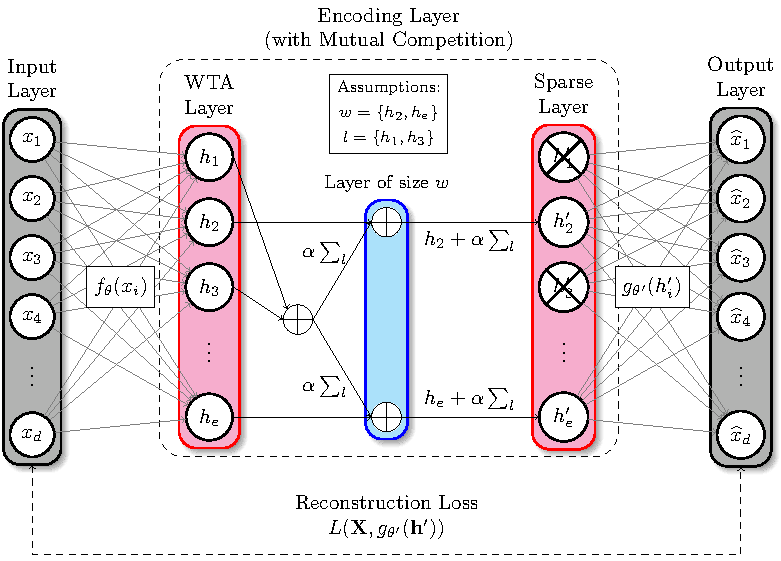
\includegraphics[width=0.65\textwidth]{ch04/mc_autoencoder}
  \caption[Mutually-competitive autoencoder architecture]
  {Mutually-competitive autoencoder}
  \label{schema:mc_autoencoder}
\end{figure}

%=============================================================================
% algo_wta.tex
% Copyright (c) 2018. Lester James V. Miranda
%
% This file is part of thesis-manuscript.
%
% thesis-mansucript is free software: you can redistribute it and/or modify
% it under the terms of the GNU General Public License as published by
% the Free Software Foundation, either version 3 of the License, or
% (at your option) any later version.
%
% thesis-manuscript is distributed in the hope that it will be useful,
% but WITHOUT ANY WARRANTY; without even the implied warranty of
% MERCHANTABILITY or FITNESS FOR A PARTICULAR PURPOSE.  See the
% GNU General Public License for more details.
%
% You should have received a copy of the GNU General Public License
% along with thesis-manuscript.  If not, see <http://www.gnu.org/licenses/>.
%
% Created by: Lester James V. Miranda <ljvmiranda@gmail.com>
%=============================================================================


\begin{algorithm}
    \caption{Winner-Take-All operation}
    \label{algo:wta}
    \begin{algorithmic}[1]
    
    \INPUT Output of last encoding layer $\mathbf{h}$, percent sparsity $k\%$
    \OUTPUT Dictionary of winners and losers, $D = \{\}$

    \item[]
    \State \textit{LayerSize} $\gets$ length($\mathbf{h}$)
    \Comment Get number of units in the layer
    \State \textit{NeuronsToKeep} $\gets k\% * \text{\textit{LayerSize}}$
    \State $D[\text{Winners}] \gets$ first \textit{NeuronsToKeep} in \Call{SortAscendingOrder}{$\mathbf{h}$}
    \State $D[\text{Losers}] \gets$ remaining neurons in \Call{SortAscendingOrder}{$\mathbf{h}$}
    \State \Return $D$
    \end{algorithmic}
\end{algorithm}


\subsection{Sparse operation}

\par The sparse operation allows the winners to ``soak-up'' the activation of
the losers. This is done via an adder controlled by a hyperparameter
$\alpha$. Boosting the energy of the winning neurons affects the
backpropagation path so that weights are optimized in their favor. This
assumes that the winners, due to their high activation, are the relevant
features representing the input data.

\par Selectively manipulating neuron activations encourages competition among
neurons. Throughout training, neurons with consistently high
activations\textemdash i.e. highly-relevant with respect to the output
reconstruction\textemdash are retained. There were some attempts in
maximizing the activation of relevant neurons in other problem
domains: this includes pruning network weights, dropout, and selectively
deleting neurons (\cite{louizos2017learning, chen2017kate, theis2018faster}).
The main difference in this method (in connection with the winner-take-all
operation), is that competition is done via the architecture itself, not as
an objective function or regularizer.

\par Boosting neuron activations is achieved by obtaining the aggregate sum
of the loser activations, and then transferring them to the winner
activations. Meanwhile, the loser activations are set to $0$. Equation
\ref{eqn:sparse_operation} illustrates this process for a layer $\mathbf{h} =
\{h_{w}, h_{l}\}_{i=1}^{d}$ mapped into a ``sparse layer''
$\mathbf{h}^{\prime} = \{h^{\prime}_w, h^{\prime}_l\}_{i=1}^{d}$. In
addition, Algorithm \ref{algo:sparse} describes the whole operation.

\begin{equation}
  \label{eqn:sparse_operation}
  h^{\prime}_{w} = h_{w} + \sum_{i=1}^{e(1-k)}h_{l,i} \quad \text{and} \quad h^{\prime}_l = 0 
\end{equation}

%=============================================================================
% algo_sparse.tex
% Copyright (c) 2018. Lester James V. Miranda
%
% This file is part of thesis-manuscript.
%
% thesis-mansucript is free software: you can redistribute it and/or modify
% it under the terms of the GNU General Public License as published by
% the Free Software Foundation, either version 3 of the License, or
% (at your option) any later version.
%
% thesis-manuscript is distributed in the hope that it will be useful,
% but WITHOUT ANY WARRANTY; without even the implied warranty of
% MERCHANTABILITY or FITNESS FOR A PARTICULAR PURPOSE.  See the
% GNU General Public License for more details.
%
% You should have received a copy of the GNU General Public License
% along with thesis-manuscript.  If not, see <http://www.gnu.org/licenses/>.
%
% Created by: Lester James V. Miranda <ljvmiranda@gmail.com>
%=============================================================================

\begin{algorithm}
    \caption{Sparse operation}
    \label{algo:sparse}
    \begin{algorithmic}[1]
    
    \INPUT Dictionary of winners and losers $D = \{\}$, competition parameter $\alpha$
    \OUTPUT Updated activation of winners and losers $\mathbf{h}'$

    \item[]
    \State \textit{ToAllocate} $\gets$ \Call{Sum}{$D[Losers]$}
    \Comment Sum all activations of loser neurons
    \State $\mathbf{a}_{w} \gets$ $D[Winners]$ + $\alpha$ \textit{ToAllocate}
    \Comment Update activation of winners, $\mathbf{a}_{w}$
    \State $\mathbf{a}_{l} \gets 0$ 
    \Comment Set activation of losers to $0$.
    \State \textbf{return} $\mathbf{h}' = \{\mathbf{a}_{w}$, $\mathbf{a}_{l}\}$
    \end{algorithmic}
\end{algorithm}


\subsection{Practical considerations for MC training}

\par In summary, the combination of the winner-take-all and sparse operations
introduces information bottlenecks when reconstructing the input data. This
should encourage the creation of sparse yet relevant features for
classification. From this design, three hyperparameters can be derived:


\begin{itemize}
  \item \textit{Number of encoding units}, $e$: controls the number of units
  in the hidden layer. If $e > d$, the autoencoder is said to be
  overcomplete, else, undercomplete.
  \item \textit{Number of winners}, $k \in \left[0,1\right]$: controls the
  number of winners retained by the winner-take-all operation.
  \item \textit{Competition parameter}, $\alpha \in \mathbb{R}$: controls the
  intensity to which the loser activations are reallocated to the winners.
  Can range from $10^{1}$ to $10^{2}$.
\end{itemize}

\vspace*{-10pt}
%=============================================================================
% algo-training.tex
% Copyright (c) 2018. Lester James V. Miranda
%
% This file is part of thesis-manuscript.
%
% thesis-mansucript is free software: you can redistribute it and/or modify
% it under the terms of the GNU General Public License as published by
% the Free Software Foundation, either version 3 of the License, or
% (at your option) any later version.
%
% thesis-manuscript is distributed in the hope that it will be useful,
% but WITHOUT ANY WARRANTY; without even the implied warranty of
% MERCHANTABILITY or FITNESS FOR A PARTICULAR PURPOSE.  See the
% GNU General Public License for more details.
%
% You should have received a copy of the GNU General Public License
% along with thesis-manuscript.  If not, see <http://www.gnu.org/licenses/>.
%
% Created by: Lester James V. Miranda <ljvmiranda@gmail.com>
%=============================================================================

\begin{algorithm}[!h]
\caption{Training the mutually-competitive autoencoder network}
\label{algo:mc_training}
\begin{algorithmic}[1]

\INPUT Training examples $\mathbf{X}$, hyperparameters $\langle\alpha, k\%, e\rangle$
\OUTPUT Learned weights, $\theta^{\ast}$

\item[]
\For{\textit{NumEpochs}}
    \State Feedforward propagation: $\mathbf{h} \gets f_{\theta}(\mathbf{X}) =
    \sigma(\theta\mathbf{X}^{T}+\theta_{0})$
    \State $D \gets$ \Call{WinnerTakeAll}{$\mathbf{h}$, $k$}
    \State $\mathbf{h'} \gets$ \Call{Sparse}{$D$, $\alpha$}
    \State Compute output: $\mathbf{\widetilde{X}} \gets 
    g_{\theta'}(\mathbf{h'}) = \sigma(\theta'\mathbf{h'}^{T}+\theta_{0})$
    \State Compute reconstruction error $L$
    \State $\theta^{\ast} \gets$ \Call{Backpropagation}{$L$}
\EndFor
\State \Return $\theta^{\ast}$ 

\end{algorithmic}
\end{algorithm}



\subsection{Relationship to other works}
\par The idea of mutual competition has been explored in other works, although
not necessarily in protein function prediction. Our work on the
mutually-competitive autoencoder serves as another brick to this long line of
research. In this section, we will differentiate it to similar implementations.
\begin{itemize}
    \item \cite{makhzani2014ksparse}'s work on k-sparse and winner-take-all
        (WTA) autoencoders also has the ability to turn-off neurons during
        training, but does not employ sparse operation. We can consider WTA as
        a special case of our model when $\alpha=0$.
    \item \cite{zhai2016semisupervised,louizos2017learning} and
        \cite{chen2017kate} explores an approach akin to
        neuron competition. However, they both require an additional
        preprocessing step during training. We don't have this extra step and
        use the $ReLU$ activation function for easier training. In addition, we
        prune from the architecture itself, not from the objective function.
    \item \cite{goodfellow2014generative}'s work on generative adversarial
        networks (GAN) may ring a bell whenever competition is mentioned, but
        our main difference is that competition is localized in the neuronal
        level. GANs ``compete'' on a network level.
\end{itemize}

\par In addition, our work is further distinguished by its domain-specific
application in protein function prediction, moreso in multilabel
classification. In the next section, we will introduce the full prediction
pipeline.

\section{Protein Function Prediction Pipeline}
\label{PFPPipeline}

\par The entire protein function prediction model consists of two stages: (1)
a \textit{feature extraction} stage that contains the mutually-competitive
autoencoder, and a (2) \textit{multi-label classification} stage that assigns
each protein sample to its respective set of functions.\footnote{This
pipeline is similar to the one we implemented using the stacked denoising
autoencoder in Chapter \ref{SDAEChapter}} During training, the model learns
the parameters $\theta$ and $W$ for the two stages separately. At inference,
matrix operations are applied to transform the input data and predict protein
functions. Figure \ref{schema:traintest_mc} shows the training and test
phases.

\begin{figure}[!t]
  \centering
  \includegraphics[width=0.90\textwidth]{ch04/schema_traintest}
  \caption[Protein function prediction pipeline]{Protein function prediction
  pipeline for the mutually-competitive autoencoder}
  \label{schema:traintest_mc}
\end{figure}
%\newpage
\begin{itemize}
  \item \textit{Training phase:} our goal during training is to learn the
  parameters $\theta$ for the feature extractor, and $W$ for the classifier.
  We simply implement the traditional training scheme for autoencoders (Alg.
  \ref{algo:autoenc}), and minimize the mean-square error, $L$ (Eq.
  \ref{eqn:loss_fe}). Then, we minimize the L2-SVM loss (Eq.
  \ref{eqn:loss_clf}) for our classifier:
  \begin{align}
    % Feature Extractor Loss
    \label{eqn:loss_fe}
    L(\mathbf{X},g_{\theta^{\prime}}(\mathbf{h}^{\prime})) &=
      \dfrac{1}{2}(\mathbf{X} - g_{\theta^{\prime}}(\mathbf{h}^{\prime}))^{2}\\
    % Multilabel classifier loss
    \label{eqn:loss_clf}
    J(\mathbf{X}^{\prime}, \widehat{\mathbf{Y}}, \mathbf{Y}) &= \sum_{\widehat{\mathbf{y}}_i \neq \mathbf{y}_{i}} \text{max}(0, W^{T}_{\widehat{\mathbf{y}}_{i}} \mathbf{x}_{i}^{\prime} - W^{T}_{\mathbf{y}_i}\mathbf{x}^{\prime}_i + \Delta)^2
  \end{align}
  \item \textit{Test phase:} upon learning the parameters $\theta^{\ast}$ and
  $W^{\ast}$, we pass our test data into the feature extractor
  $f_{\theta^{\ast}}$ (Eq. \ref{eqn:encoder_mc})\textemdash turning-off the WTA and sparse
  operations\textemdash and classify the resulting features using
  $\mathcal{H}$.
  \begin{align}
    % Encoder equation
    \label{eqn:encoder_mc}
    f_{\theta^{\ast}}(\mathbf{X}_{ts}) = \theta^{\ast T} \mathbf{X}_{ts} + \theta_{0}^{\ast}
  \end{align}
\end{itemize}


\subsection{Evaluation metrics}

After testing, we now have a set of predictions $\mathbf{\widehat{Y}}_{ts}$
to compare against a held-out ground-truth labels $\mathbf{Y}_{ts}$. To
evaluate the performance of the prediction model, we will use the following
metrics\footnote[2]{\textit{tp}: true positive, \textit{fp}: false positive,
\textit{tn}: true negative, \textit{fn}: false negative}:

\begin{align}
    \text{Hamming Loss (H)} &= \dfrac{1}{N \cdot L} \sum_{i=1}^{N} \sum_{j=1}^{L}
    \text{XOR}(y_{ij}, \widehat{y}_{ij}) \\
    \text{Precision (P)} &=
    \dfrac{1}{N}\sum_{i=1}^{N}\dfrac{|\mathbf{\widehat{y}}_{i} \cap
    \mathbf{y}_{i}|}{|\mathbf{\widehat{y}_{i}}|} = \dfrac{tp}{tp + fp} \\
    \text{Recall (R)} &=
    \dfrac{1}{N}\sum_{i=1}^{N}\dfrac{|\mathbf{\widehat{y}}_{i} \cup
    \mathbf{y}_{i}|}{|\mathbf{\widehat{y}_{i}}|} = \dfrac{tp}{tp + fn} \\
    \text{F-score (F)} &=
    \dfrac{1}{N}\sum_{i=1}^{N} \dfrac{2 | \mathbf{\widehat{y}}_{i} \cup
        \mathbf{y}_{i}|}{|\mathbf{\widehat{y}}_{i} | + |\mathbf{y}_{i}|} =
        \dfrac{2 (\text{P} \cdot \text{R})}{\text{P} +
        \text{R}}
\end{align}

\par We will also compute for a fifth metric, the Area Under the ROC Curve
(AUROC), to serve as proxy for accuracy. Together with the Hamming loss and
F-score, the model will be evaluated and compared to other works. Lastly, the
Precision-Recall score will determine the quality of our model in terms of
sensitivity and specificity. This time, we will obtain the micro, macro, and
samples average for the AUROC and F-score, enabling us to further gauge model
performance.

\section{Experimental Set-up}
\label{MCExperiments}

There are two experimental themes in this work. First, we characterized the
proposed autoencoder by examining how each hyperparameter, $\langle e, k\%,
\alpha \rangle$, affects the classifier's ability to discriminate samples.
Then, we conducted experiments to test our hypotheses on feature relevance and
prediction performance. A summary of all experiments can be seen in Tables
\ref{exp:hyperparameter} and \ref{exp:key_results}.

\begin{table}[!h]
  \centering
  \caption{Summary of experiments for autoencoder characterization}
  \label{exp:hyperparameter}
      \begin{tabular}{@{}rp{0.65\textwidth}@{}}
          \toprule
          Hyperparameter                      & Description \\ \midrule
          Nb. of encoding units, $e$    & Test overcomplete and undercomplete configurations.\\
          Nb. of winners, $k\%$     & Sweep $k$-values in the range $\left[ 0,1\right]$\\
          Competition parameter, $\alpha$ & Rough search from $\num{1e-3}$ to $\num{1e3}$\\ \bottomrule
      \end{tabular}
\end{table}

\begin{table}[!h]
  \centering
  \caption{Summary of experiments for analysis and benchmarking}
  \label{exp:key_results}
  \begin{threeparttable}
      \begin{tabular}{@{}rp{0.65\textwidth}@{}}
          \toprule
          Experiment                      & Description \\ \midrule
          Estimating feature relevance    & Obtained a distribution of feature scores by growing a decision tree on the features\tnote{1} \\
          Model quality         & Plotted ROC and PR curves for both
          datasets\tnote{2}\\
          Benchmark analysis     & Compared proposed model against other
          techniques in literature\tnote{3}\\
          Ablation test                   & Investigated the necessity of adding
          mutual competition in the traditional autoencoder\\\bottomrule
      \end{tabular}
  \begin{tablenotes}
      \footnotesize
      \item[1] Score distribution is normalized and averaged across all labels.
      \item[2] ROC - Receiver Operating Characteristic, PR - Precision--Recall
      \item[3] Friedman's test \parencite{friedman1937use} and post-hoc Bonferroni-Holm test \parencite{holm1979simple}
      were employed to measure statistical significance as recommended by \cite{demsar2006statistical}.
  \end{tablenotes}
  \end{threeparttable}
\end{table}

\par Lastly, Table \ref{exp:implementation} describes the implementation
environment for running the tests. The neural network was trained on an
NVIDIA Titan X (Pascal) GPU while the classifier was fitted using an Intel
Xeon 2.2GHz CPU. The majority of the code was written in Python 3.6.X using
the \href{https://www.tensorflow.org/}{Tensorflow} and
\href{https://keras.io/}{Keras} package\footnote{For more information on how
the classifier was trained and how the software package was used, please see
the Appendix}.

\begin{table}[!h]
  \centering
  \caption{Experimental environment}
  \label{exp:implementation}
  \begin{threeparttable}
  \begin{tabular}{@{}rp{0.70\textwidth}@{}}
      \toprule
      Environment                    & Value                                             \\ \midrule
      \textit{Validation and testing}                                                    \\
      Number of trials               & 10: mean and std. dev. reported                   \\
      Train--validation--test split  & 50--30--20                                        \\ \cmidrule{1-2}
      \textit{Hardware dependencies}                                                     \\
      Number of cores\tnote{1}       & 10 in use (40 maximum)                            \\
      CPU                            & Intel Xeon 2.2GHz: Classifier training            \\
      GPU                            & NVIDIA Titan X (PASCAL): Neural network training  \\ \cmidrule{1-2} 
      \textit{Software dependencies}                                                     \\
      Package Name                   & PFPredict\tnote{2}                                \\
      Language                & Python 2.7, 3.6 (compatible to both versions)            \\
      Libraries               & Tensorflow 1.2.1, Keras 2.1.2, Numpy 1.14.2              \\ \bottomrule
  \end{tabular}
  \begin{tablenotes}
    \footnotesize
    \item[1] We implemented a distributed scheme for training the classifier.
    Please see Appendix \ref{AppendixDistributed}.
    \item[2] PFPredict is a small package we developed for the mutually-competitive autoencoder.
    Please see Appendix \ref{AppendixPFPredict}.
  \end{tablenotes}
  \end{threeparttable}
\end{table}

\section{Results and Discussion}
\label{MCResults}

\par This section presents the experimental results listed in Tables
\ref{exp:hyperparameter} and \ref{exp:key_results}. Again, we'll first
investigate how different hyperparameter settings, namely, $e$, $k\%$, and
$\alpha$, affect the model's predictive performance for the two protein
benchmarks. Then, we'll test our claims using various experiments listed in
Table \ref{exp:key_results}. Remember that our main hypothesis states that the
features extracted by the mutually-competitive autoencoder are
\textit{relevant}, and should result to better predictions for the multilabel
classifier.

%\newpage
\subsection{Characterizing the autoencoder model}

In this experiment, we tested how different hyperparmeter settings affect the
model as a whole. We'll be using the Area under the ROC curve as our main
metric. The procedure is simple: change a specific hyperparameter
$\mathcal{P}$ and measure the resulting AUROC while keeping other variables
constant. We redo this process for different values of $\mathcal{P}$. 

\par Note that these experiments were performed to find a pattern on model
behavior given a dataset. Once these patterns are determined, a fine-search
(\cite{bergstra2012random}) is conducted to get the actual values. The
implementation details can be seen in Appendix \ref{AppendixImplementation}.

\subsubsection{Experiments on the Yeast Dataset}

Figure \ref{results:mc_benchmark_yeast} shows the results for Yeast. Recall
that validation set performance should always be lower than training set
performance, as the former simulates unseen samples. Here we can observe the
following:

\begin{itemize}
  \item An overcomplete autoencoder ($e=500$) gives the optimal validation
  set performance. However, adding more hidden units tends to overfit the
  model.
  \item The amount of winners to keep should not be too high ($k=1.00$) nor
  too low ($k=0.00$). Here, we see an optimal value in the middle range
  ($k\in\left[0.33, 0.67\right]$).
  \item The value of $\alpha$ should not be excessively high nor excessively
  low. A value between \num{1e0} to \num{100} should suffice.
\end{itemize}

\begin{figure}[!h]
  \centering
  \includegraphics[width=0.95\textwidth]{ch04/hyperparams_yeast}
  \caption{Model behavior on the Yeast Dataset}
  \label{results:mc_char_yeast}
\end{figure}

\subsubsection{Experiments on the Genbase Dataset}

Figure \ref{results:mc_char_genbase} shows the results for Genbase. A similar
procedure was performed for both training and validation data. We can infer
the following from the plots:

\begin{itemize}
  \item An undercomplete autoencoder ($e\in\left[50,100\right]$) gives the
  optimal validation set performance. A large value can damage the model (e.g.,
  $e=2000$).
  \item Similar to the Yeast dataset, the amount of winners should be
  moderated. Although lower values are preferred, setting them too low can
  potentially damage the model.
  \item The competition parameter $\alpha$ can be set at a lower value (around
  $\alpha \in \left[1,10\right]$). Increasing this value further only gives
  marginal benefits.
\end{itemize}

\begin{figure}[!h]
  \centering
  \includegraphics[width=0.95\textwidth]{ch04/hyperparams_genbase}
  \caption{Model behavior on the Genbase Dataset}
  \label{results:mc_char_genbase}
\end{figure}

\subsection{Key results for the mutually-competitive autoencoder}

Throughout this work, our main hypothesis states that the features extracted by
the proposed autoencoder are relevant, thus giving better predictions when
fed to a multilabel classifier. In this section, we will present key results
testing this claim.

\subsubsection{Examining feature relevance}

\par Decision trees were proven to provide reliable information regarding a
feature's importance during classification (\cite{kazemitbar2017variable}).
Thus, to quantify feature relevance, we trained a decision tree
$\mathcal{T}(\mathcal{X}, \mathcal{Y})$ to obtain a set of feature scores
$\mathcal{S} = \{s_{i}\}_{i=1}^{N}$ for each feature ${x}_{i}$. Then, we
normalized the scores between $0$ and $1$ and plotted their distribution on a
histogram. We performed this experiment for both raw attributes
$\mathcal{T}_{1}(\mathcal{X}=\mathbf{X}, \mathcal{Y}=\mathbf{Y})$ and
extracted features $\mathcal{T}_{2}(\mathcal{X}=\mathbf{X}^{\prime},
\mathcal{Y}=\mathbf{Y})$. Figure \ref{results:mc_score_distribution} shows
the feature score distribution for both datasets.

\begin{figure}[!h]
  \centering
  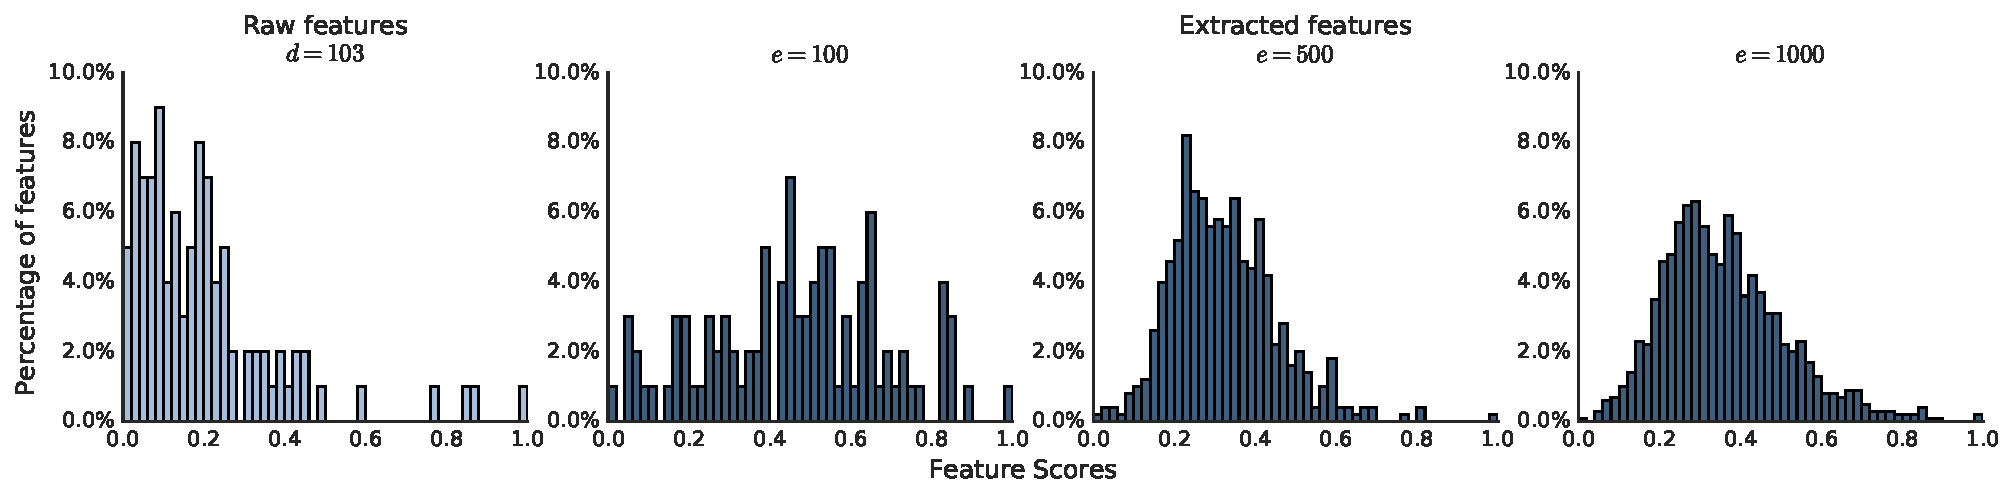
\includegraphics[width=0.95\textwidth]{ch04/fi_yeast}
  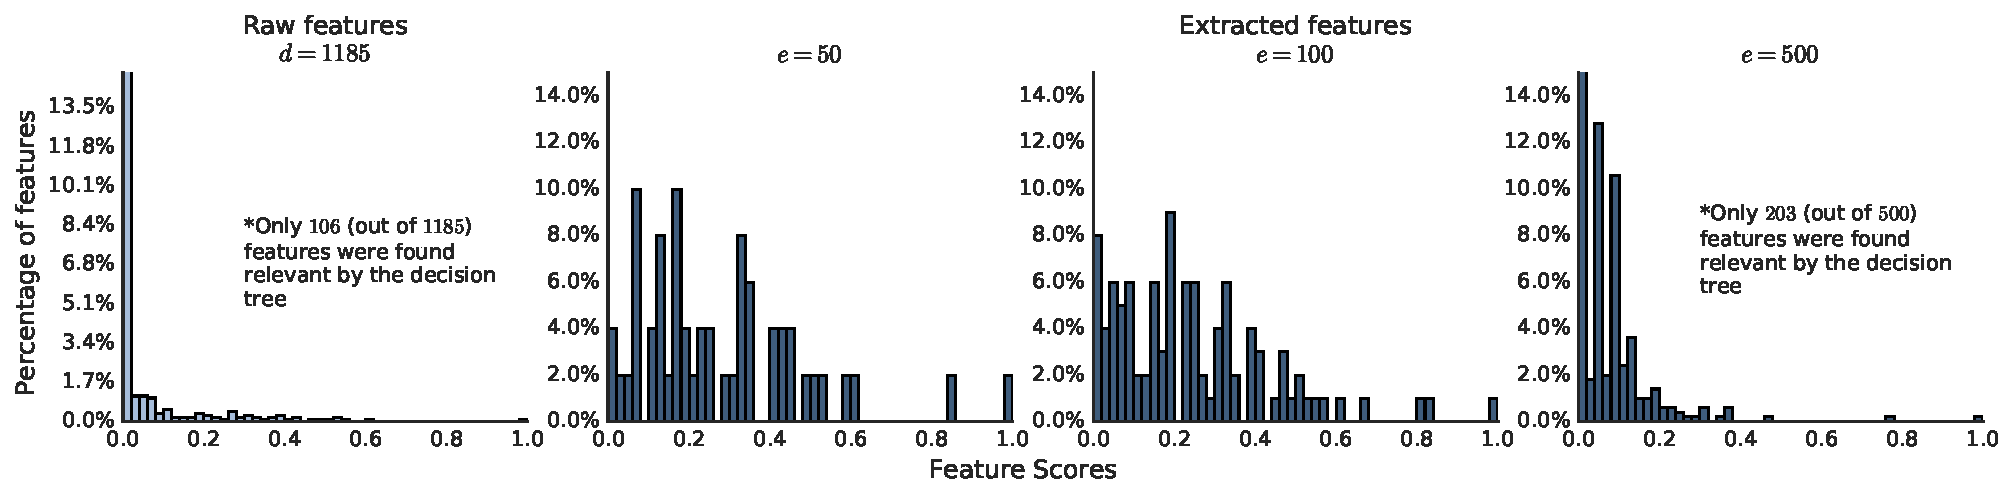
\includegraphics[width=0.95\textwidth]{ch04/fi_genbase}
  \caption[Feature score distribution for the two protein benchmarks]{
    Feature score distribution for both Yeast (\textit{top}) and Genbase
    (\textit{bottom}) datasets for different number of encoding units.
  }
  \label{results:mc_score_distribution}
\end{figure}

\par The feature score distribution for the raw attributes is colored
light-blue. It is evident that for both datasets, the distribution lies on
the lower value-range. This is especially true for Genbase, with only a small
fraction of features found relevant. This suggests that given a
classification task, the current feature space will not perform
well.\footnote{This is further validated by benchmark comparisons in later
experiments} However, the score distribution shifted to a higher-range upon
using the extracted features. This behavior is consistent for different
encoding units. This suggests that with respect to the classification task,
the extracted features are important and contributes well in achieving better
predictive performance.

\subsubsection{Assessing model quality}

This experiment serves as a ``sanity-check'' to test if the extracted
features are indeed suitable for classification. After obtaining new features
from the mutually-competitive autoencoder, they were used as input to a
BR-SVM classifier for prediction. Then, we drew Receiver Operating
Characteristic (ROC) and Precision-Recall (PR) curves as shown in Figure
\ref{results:mc_quality}. We plotted test set performance for the overall
model and for five (5) random labels for completeness.

\begin{figure}[!h]
  \centering
  \includegraphics[width=0.95\textwidth]{ch04/ql_yeast}
  \includegraphics[width=0.95\textwidth]{ch04/ql_genbase}
  \caption[Receiver Operating Characteristic (ROC) and Precision-Recall (PR)
  curves for the two protein benchmarks]{
    Receiver Operating Characteristic (ROC) and Precision-Recall (PR) curves
    for both Yeast (\textit{top}) and Genbase (\textit{bottom}) datasets.
  }
  \label{results:mc_quality}
\end{figure}

\par The easiest way to interpret ROC curves is to check how far the curve is
from the dotted line.\footnote{This line represents the performance of a
random classifier. Only inside this scope, we will call this as the
baseline.} For both datasets, we can see that the orange curve is way above
the baseline, moreso with Genbase. This indicates that the classifier can
decently predict protein functions using the extracted features. On the other
hand, the PR curves reflect the precision-recall tradeoff for both datasets.
We can qualitatively gauge the optimal point where both precision and recall
are at their maximum by finding the vertex of the curve. For Yeast, this is
when Precision $P = 0.742$ and for Genbase, when $P=0.988$. In the next
section, we'll bring these results into context by comparing our model (i.e.,
feature extractor with the classifier) to other models in literature.

\subsubsection{Benchmark analysis}

\par In this experiment, we compared against similar techniques in literature.
We ran the models for ten (10) trials, and reported test set performance. In
addition, we performed post-hoc statistical tests to check if the differences
between groups are significant. Tables \ref{results:mc_benchmark_yeast} and
\ref{results:mc_benchmark_genbase} show the results.

\par Here, the baseline method corresponds to a model without feature
extraction. The raw attributes were directly fed to the BR-SVM classifier for
inference. This enables us to check if there is any performance difference
between the extracted features and the raw attributes. The ``Sig.'' column
indicates the extent in $\alpha$ in which the null hypothesis $H_{0}$ is
rejected. We implemented the Friedman's ranking test to compute for
$p$-values (\cite{friedman1937use, demsar2006statistical}). For Friedman's
test, $H_{0}$ states that there is no significant difference between groups.

\begin{table}[t]
%
\centering
\begin{threeparttable}
\caption{Benchmark analysis on Yeast dataset}
\label{results:mc_benchmark_yeast}
%
\begin{tabular}{@{}rr*{6}{l}@{}}
\toprule
        & & \multicolumn{5}{c}{Prediction Model\tnote{1}} \\ \cmidrule{3-7}
Metrics & Avg. & Baseline & M1 & M2 & M3 & Proposed\tnote{2} &
Sig.\tnote{3}\\
\midrule
AUROC & micro & \num{0.667(3)} & \num{0.666(2)} & \num{0.643(1)} &
\num{0.668(4)} & \hg \num{0.732(2)} & *** \\
        & macro & \num{0.655(3)} & \num{0.659(2)} & \hg \num{0.662(1)} &
        \num{0.648(2)} & \num{0.646(2)} & ** \\
        & sample & \num{0.670(3)} & \num{0.656(2)} & \num{0.643(1)} &
        \num{0.657(3)} & \hg \num{0.743(4)} & *** \\
F-score & micro & \num{0.548(4)} & \num{0.538(2)} & \num{0.530(1)} &
\num{0.579(3)} & \hg \num{0.629(3)} & *** \\
        & macro & \num{0.597(4)} & \num{0.603(2)} & \num{0.590(1)} &
        \num{0.613(2)} & \hg \num{0.630(2)} & *** \\
        & sample & \num{0.536(3)} & \num{0.524(2)} & \num{0.517(1)} &
        \num{0.572(3)} & \hg \num{0.609(4)} & *** \\
Hamming Loss & -- & \num{0.322(2)} & \num{0.343(2)} & \num{0.354(1)} &
\num{0.231(3)} & \hg \num{0.224(2)} & *** \\
\bottomrule
\end{tabular}
%
\begin{tablenotes}
        \footnotesize
    \item[1] M1: \cite{wang2013protein}, M2: \cite{chicco2014deep}, M3: \cite{miranda2017feature}
    \item[2] Feature ext.: $\{e=500,\alpha=10.0,k=0.6\}$, BR-SVM: $\{C=\num{1.00}, \gamma=\num{1.63e-3}\}$
    \item[3] Significance: *-$p\leq 0.1$, **-$p\leq 0.05$, ***-$p\leq 0.01$
\end{tablenotes}
%
\end{threeparttable}
%
\end{table}

\begin{table}[t]
%
\centering
\begin{threeparttable}
\caption{Benchmark analysis on Genbase dataset}
\label{results:mc_benchmark_genbase}
%
\begin{tabular}{@{}rrllllll@{}}
\toprule
        &       &  \multicolumn{5}{c}{Prediction Model\tnote{1}} \\ \cmidrule{3-7}
Metrics & Avg.  & Baseline       & M1             & M2             & M3               & Proposed\tnote{2}  & Sig.\tnote{3}\\
\midrule
AUROC     & micro    & \num{0.856(0)} & \num{0.987(0)} & \num{0.974(10)} & \num{0.987(1)}  & \hg \num{0.999(0)}  & ***  \\
        & macro    & \num{0.671(0)} & \num{0.992(0)} & \num{0.979(11)} & \num{0.983(1)}  & \hg \num{0.999(0)}  & ***  \\
        & sample    & \num{0.613(0)} & \num{0.950(0)} & \num{0.976(10)} & \num{0.988(1)}  & \hg \num{0.999(0)}  & ***  \\
F-score & micro    & \num{0.671(0)} & \num{0.887(1)} & \num{0.785(87)} & \num{0.962(11)} & \hg \num{0.986(7)}  & ***  \\
        & macro    & \num{0.716(0)} & \num{0.950(0)} & \num{0.892(40)} & \num{0.964(6)}  & \hg \num{0.992(2)}  & ***  \\
        & sample    & \num{0.760(0)} & \num{0.928(0)} & \num{0.810(95)} & \num{0.970(8)}  & \hg \num{0.989(6)}  & ***  \\
Hamming Loss   & --    & \num{0.041(0)} & \num{0.014(2)} & \num{0.035(17)} & \num{0.005(1)}  & \hg \num{0.002(0)}  & ***  \\
\bottomrule
\end{tabular}
%
\begin{tablenotes}
    \footnotesize
    \item[*] Values with $0.XXX(0)$ stdev. have deviations in the ten-thousandths place 
    \item[1] M1: \cite{wang2013protein}, M2: \cite{chicco2014deep}, M3: \cite{miranda2017feature}
    \item[2] Feature ext.: $\{e=30,\alpha=5.32,k=0.6\}$, BR-SVM: $\{C=\num{1.00}, \gamma=\num{1.24e-3}\}$
    \item[3] Significance: *-$p\leq 0.1$, **-$p\leq 0.05$, ***-$p\leq 0.01$
\end{tablenotes}
%
\end{threeparttable}
%
\end{table}


\par It is highly-evident that the mutually-competitive autoencoder performed
better in comparison to other models by a significant margin. It also
outperformed the Baseline across all metrics, validating our claim that using
extracted features\textemdash especially those from the proposed
autoencoder\textemdash can lead to better predictive performance. Lastly, we
conducted a post-hoc Bonferroni-Holm (\cite{holm1979simple}) test to compare
each model against each another using the results from both datasets. Table
\ref{results:mc_stats} shows this comparison. The $p$-values indicate that the
proposed model, when accounting for all metrics in both datasets, performs
significantly better than other techniques in literature.

\begin{table}[t]
%
\centering
\begin{threeparttable}
\caption{One-vs-All Overall Comparison\\using post-hoc Bonferroni-Holm Test\tnote{1}}
\label{results:mc_stats}
%
\begin{tabular}{@{}r*{3}{l}@{}}
\toprule
Proposed Model vs.                       & Z-statistic    & $p$-value         & Sig.\tnote{2} \\ \midrule
Baseline                                 & $4.54187$      & $0.00002$         & ***           \\
\cite{wang2013protein}                   & $3.28688$      & $0.00203$         & ***           \\
\cite{chicco2014deep}                    & $4.78091$      & $0.00001$         & ***           \\
\cite{miranda2017feature}                & $1.73308$      & $0.08308$         & *             \\ \bottomrule
\end{tabular}
\begin{tablenotes}
\footnotesize
\item[1] Friedman's test rejects $H_{0}$ with $\chi^{2}=\num{17.71730}$.
\item[2] Significance: *-$p\leq0.1$, **-$p\leq0.05$, ***-$p\leq0.01$
\end{tablenotes}
\end{threeparttable}
\end{table}


\subsubsection{Ablation tests}

\par In this experiment, we test if our modifications to the traditional
autoencoder are beneficial to the model's predictive performance.  We start
from a source configuration, then incrementally add components until we reach
the target configuration. We begin with a traditional autoencoder as our
source, then add the winner-take-all (WTA) and sparse (SL) operations until we
achieve the target architecture. For each step, we evaluate using the Area
under the ROC curve. Figure \ref{results:mc_ablation} shows the results.

\begin{figure}[t]
  \centering
  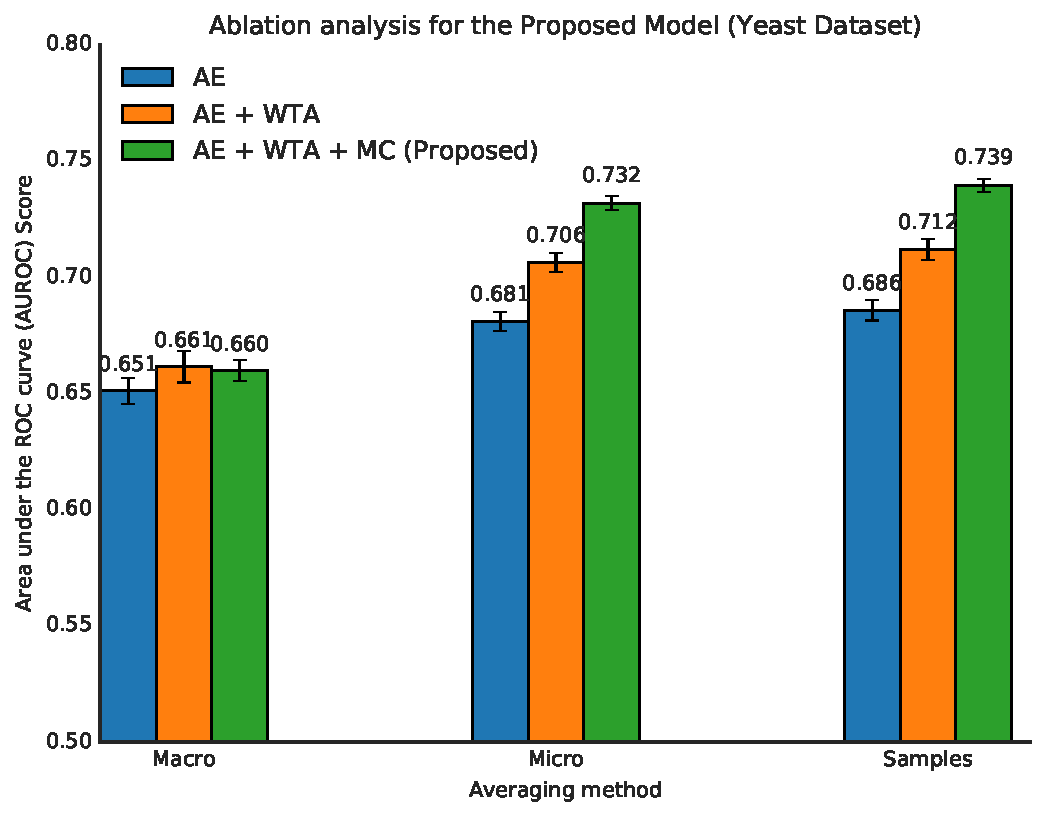
\includegraphics[width=0.38\textwidth]{ch04/ab_yeast}
  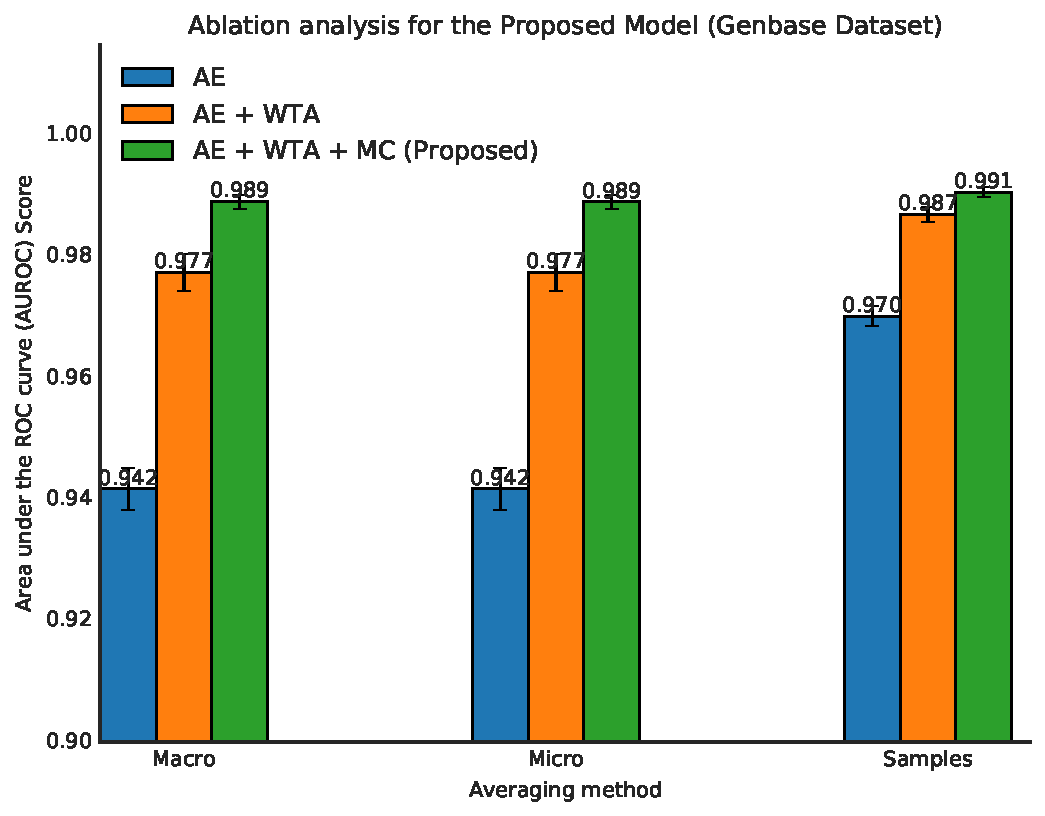
\includegraphics[width=0.38\textwidth]{ch04/ab_genbase}
  \caption[Ablation test results for the two protein benchmarks]{
    Ablation test results (Area under the ROC curve)
    for both Yeast (\textit{left}) and Genbase (\textit{right}) datasets.
  }
  \label{results:mc_ablation}
\end{figure}

\par It is evident that as we add components to the traditional autoencoder,
the performance of the predictor improves. There is a sharp increase from AE
upon addition of WTA, suggesting that the bottleneck improves model
performance. Winner-take-all keeps the highly-activated neurons, and using them
for feature extraction serves a beneficial purpose. More importantly, there is
also a performance increase when the sparse operation was added to the WTA
set-up. Manipulating the information flow has helped improve model accuracy,
and gave empirical weight to the efficacy of our method. Overall, the above
results prove that mutual competition is indeed essential to achieve high
predictive performance.

\section{Conclusion}
\label{MCConclusions}

\par To extract task-relevant and meaningful representations of data for
predicting protein functions, we designed a mutually-competitive autoencoder
architecture.  Our proposed method shares some similarities with the
traditional autoencoder, but has an additional layer consisting of
winner-take-all and sparse operations. Together, they encourage neurons that
best represent the input to be activated throughout training. We hypothesize
that the feature extractor should be able to derive task-relevant features, and
in consequence, boost a multilabel classifier's predictive performance.

\par The proposed autoencoder was tested on the Yeast and Genbase protein
benchmarks. First, we investigated how different hyperparameter settings
affect the model as a whole. The number of encoding units $e$ generally
depends on the dataset itself, with Yeast benefitting from overcomplete
configurations while Genbase for undercomplete architectures. However, the
top-$k\%$ neurons for the winner-take-all operation were seen to be optimal
at low values. This suggests that constraining the hidden layer helps
representation of data. Lastly, the intensity of competition, $\alpha$, is
helpful when set to a certain value. Very high values of $\alpha$ (in the
order of $10^{2}$ or $10^{3}$) only gives marginal returns. It is helpful to
note that finding values for $k$ and $\alpha$ is beneficial than setting
$k=1$ (keep all neurons) or $\alpha=0$ (no competition).

\par Next, we conducted experiments to test our claim. By training a decision
tree, the feature scores for the extracted features are much higher than
those of the raw attributes. Then, via a thorough comparison of the proposed
model with other techniques in literature, we saw that our model outperforms
most works by a significant margin. More importantly, the autoencoder has
greater performance than the baseline, further supporting our claim that
extracting features is more beneficial. Lastly, we performed ablation tests
to check if the modifications we've added to the traditional autoencoder
affects a model's predictive accuracy. The trendlines for both datasets show
that mutual competition in general benefits a classifier's performance.

\par This work validates the claim that extracting task-relevant features can
lead to better classification. In our case, we have demonstrated that the
mutually-competitive autoencoder performs task-relevant feature extraction.
The performance of the classifier when using the task-relevant features is
higher than just using raw attributes or extracted features from naive
methods.

%=============================================================================
% Conclusion
% Copyright (c) 2018. Lester James V. Miranda
%
% This file is part of thesis-manuscript.
%
% thesis-mansucript is free software: you can redistribute it and/or modify
% it under the terms of the GNU General Public License as published by
% the Free Software Foundation, either version 3 of the License, or
% (at your option) any later version.
%
% thesis-manuscript is distributed in the hope that it will be useful,
% but WITHOUT ANY WARRANTY; without even the implied warranty of
% MERCHANTABILITY or FITNESS FOR A PARTICULAR PURPOSE.  See the
% GNU General Public License for more details.
%
% You should have received a copy of the GNU General Public License
% along with thesis-manuscript.  If not, see <http://www.gnu.org/licenses/>.
%
% Created by: Lester James V. Miranda <ljvmiranda@gmail.com>
%=============================================================================
\chapter{Conclusion}
\label{ConclusionsChapter}

\par In this work, we have tackled the protein function prediction problem in
the angle of feature extraction: if we can extract \emph{better} features, then
we can obtain better predictions. Better features mean task-relevant and
meaningful representations of data, and by Def. \ref{DefRelevance}, can be
measured with an improvement in classification performance. 

\par Hence, we presented two autoencoder-based approaches geared towards the
extraction of relevant features: (1) a stacked denoising autoencoder-based
model that sifts through noise to obtain relevant features and (2) a
mutually-competitive autoencoder architecture that derives sparse yet relevant
representations. Our main hypothesis states that by using these methods, we can
generate relevant features, thereby inducing greater classification
performance. We tested our hypothesis on two protein benchmarks, Yeast and
Genbase, in a multilabel setting. There are two key insights in our work:


% Extracting relevant features is indeed crucial
\paragraph{Learning relevant features has benefit to classification.} Features
extracted from our two models have superior performance than other techniques
in literature. Specifically, we outperformed a dimensionality-reduction
approach (PCA) and a regular feature extractor (traditional autoencoder). More
importantly, we surpassed a baseline method without feature extraction. This
shows that although learning new representations is important, mere feature
extraction is not enough. In addition, we have demonstrated that it is
worthwhile to extract features first before inference. Most importantly, it is
crucial to ensure that the features we are deriving are relevant to the task at
hand. 

% Mutually-competitive autoencoder outperforms stacked denoising autoencoder
\paragraph{The mutually-competitive architecture outperforms the stacked
denoising autoencoder in most metrics} The architecture we designed in Chapter
\ref{SelectiveChapter} has greater performance than the stacked denoising
autoencoder (SdAE) in Chapter \ref{SDAEChapter} with respect to our problem
domain. We suggest two explanations for this behavior. First, the MC
autoencoder adds a higher degree of control during feature extraction. Aside
from the architecure, we can set three different hyperparameters to dictate the
flow of information in our network. Second, the autoencoder's strength lies on
its ability to prevent information loss while preserving data from the original
inputs. As we've seen in our ablation tests, the competition parameter that
reallocates neuron activations after winner-take-all has been beneficial to the
classifier's predictive performance. Thus, we not only learn the manifold, but
preserve more information to the relevant neurons.

\newpage
\par Next, we would like to list down the merits and major contributions of our
research:
\begin{itemize}
    \item In Chapter \ref{SDAEChapter}, we have successfully demonstrated the
        transferability of the stacked denoising autoencoder, commonly-used in
        images, to protein data within a multilabel setting. Learning the
        manifold via small perturbations in the input has been beneficial. More
        bottlenecks can lead to better generalization.
    \item In Chapter \ref{SelectiveChapter}, we have proposed an autoencoder
        architecture capable of extracting task-relevant representations of
        data. We have tested this on protein benchmarks and obtained good
        results. This architecture gives finer control during extraction, and
        performs even better than the denoising autoencoder approach.
    \item Overall, we have validated our claim that by extracting relevant
        features, we can improve the performance of a multilabel classifier in
        the protein domain. We obtained better performance when we're
        consciously extracting task-relevant features than by simple
        dimensionality-reduction or feature learning techniques.
\end{itemize}

\par In addition, it is also necessary to discuss some limitations in our work.
These can provide good jump-off points for further research:
\begin{itemize}
    \item \textit{It is difficult to interpret the extracted features from both
        models.} Although we know that these features help the classifier, it
        is difficult to distinguish what they truly represent (cell binding
        sites, sequence length, etc.). By nature, neural network models are
        black-boxes, and if we're optimizing for accuracy, we might sacrifice
        interpretability.
    \item \textit{Our work does not cover hierarchical labels.} There may be
        cases when labels also have a relationship with one another: a
        ``husky'' is a ``dog'' as ``cellular bud site selection'' is a
        ``mitotic cell cycle process.'' Our protein benchmarks all have flat
        labels, and thus these cases were not considered. 
\end{itemize}

\par Lastly, here are some suggestions for future work:
\begin{itemize}
    \item \textit{Better model interpretability for autoencoder networks.} This
        is a huge area of research and may involve the use of generative
        methods such as variational autoencoders.
    \item \textit{Improve handling of data imbalance.} There are cases when one
        label is more dominant to the other, affecting classification
        performance. A more balanced dataset can boost classifier performance.
    \item \textit{Consider label information during autoencoder training.} This
        is relevant when hierarchical labels are involved. Our feature
        extractor is unsupervised, and it may be interesting to see a
        supervised approach to autoencoder training.
\end{itemize}

\par Applying machine learning to the problem of protein function prediction is
a herculean task. It requires careful thought not only in classifying
multilabel data, but also of how proteins are represented to the classifier.
We have shown that by procuring task-relevant protein representations, we can
aid the classification of protein functions. We hope that through our methods,
we can add value to this fundamental task, and pave way to the development of
advanced medicine and better healthcare for the society. $\blacksquare$



%------------------------------------------------------------------------------
%	THESIS CONTENT - APPENDICES
%------------------------------------------------------------------------------

\appendix % Cue to tell LaTeX that the following "chapters" are Appendices

%=============================================================================
% Implementation Details Appendix
% Copyright (c) 2018. Lester James V. Miranda
%
% This file is part of thesis-manuscript.
%
% thesis-manuscript is free software: you can redistribute it and/or modify
% it under the terms of the GNU General Public License as published by
% the Free Software Foundation, either version 3 of the License, or
% (at your option) any later version.
%
% thesis-manuscript is distributed in the hope that it will be useful,
% but WITHOUT ANY WARRANTY; without even the implied warranty of
% MERCHANTABILITY or FITNESS FOR A PARTICULAR PURPOSE.  See the
% GNU General Public License for more details.
%
% You should have received a copy of the GNU General Public License
% along with thesis-manuscript.  If not, see <http://www.gnu.org/licenses/>.
%
% Created by: Lester James V. Miranda <ljvmiranda@gmail.com>
%=============================================================================

\chapter{Implementation Details}
\label{AppendixImplementation}

\par In this chapter, we'll list down necessary details regarding the
implementation of our experiments. Note that the ``$\star$'' symbol represents
a dependent variable. Lastly, we implemented grid search and a fine random
search to obtain optimal values for the BR-SVM classifier.

\section{Hyperparameters used on SdAE experiments}
\par The tables below correspond to the experiments listed in Section
\ref{SDSetup}. When testing the effect of various hyperparameters,
we kept the network and training time at a minimum.

\begin{table}[!h]
%
\centering
\caption{Hyperparameters for SdAE model characterization}
%
\begin{tabular}{@{}rr*{9}{l}@{}}
\toprule
      &  && \multicolumn{5}{c}{Feature Extractor} && \multicolumn{2}{c}{Classifier} \\ \cmidrule{4-8} \cmidrule{10-11}
Experiment     & Dataset && $e$     & $r$ & optimizer & epochs & reg.       && $C$       & $\gamma$  \\\midrule
Encoding units & Yeast   && $\star$ & 0.6 & Adam      & 200    & \num{1e-2} && \num{1.0} & \num{0.01} \\
               & Genbase && $\star$ & 0.6 & Adam      & 100    & \num{1e-2} && \num{1.0} & \num{0.02} \\
Noise rate     & Yeast   && 75  & $\star$ & Adam      & 200    & \num{1e-2} && \num{1.0} & \num{0.01} \\
               & Genbase && 50  & $\star$ & Adam      & 100    & \num{1e-2} && \num{1.0} & \num{0.02} \\\bottomrule
\end{tabular}
\end{table}



\par Here are the implementation details for the benchmarking part of the
experiments. To fully optimize the values, we conducted another round of grid
and random search for the BR-SVM hyperparameters, and a fine random search
for the noise rate based from the findings during characterization.

\begin{table}[!h]
%
\centering
\caption{Additional hyperparameters for SdAE model benchmarks}
%
\begin{tabular}{@{}r*{9}{l}@{}}
\toprule
        && \multicolumn{5}{c}{Feature Extractor} && \multicolumn{2}{c}{Classifier} \\ \cmidrule{3-7} \cmidrule{9-10}
Dataset && $r$        & optimizer & epochs & batch & reg.       && $C$         & $\gamma$       \\\midrule
Yeast   && $0.7451$   & Adam      & 1000   & 200   & \num{1e-2} && \num{1.00}  & \num{1.292e-2} \\
Genbase && $0.5988$   & Adam      & 750    & 100   & \num{1e-2} && \num{1.66e2}& \num{2.154e-4} \\\bottomrule
\end{tabular}
\end{table}

\begin{table}[!h]
    \centering
    \caption{Network architectures for SdAE model benchmarks}
    \begin{tabular}{@{}r*{4}{l}@{}}
    \toprule
    Dataset & Layer Name     & Shape        & Type          & Activation          \\ \midrule
    yeast   & inputLayer     & (None, 103)  & Input         & -                   \\
            & noiseLayer     & (None, 103)  & Noise         & -                   \\
            & encLayer1      & (None, 100)  & Dense         & Sigmoid             \\
            & encLayer2      & (None, 80)   & Dense         & Sigmoid             \\
            & decLayer1      & (None, 100)  & Dense-tied    & Linear              \\
            & decLayer2      & (None, 103)  & Dense-tied    & Linear              \\ \midrule
    genbase & inputLayer     & (None, 1186) & Input         & -                   \\
            & noiseLayer     & (None, 1186) & Noise         & -                   \\
            & encLayer       & (None, 50)   & Dense         & Linear              \\
            & decLayer       & (None, 1186) & Dense-tied    & Linear               \\ \bottomrule
    \end{tabular}
\end{table}



\newpage
\section{Hyperparameters used on MC experiments}
\par The tables below correspond to the experiments listed in Section
\ref{MCExperiments}. When testing the effect of various hyperparameters, we
kept the network and training time at a minimum. The default values during
characterization were obtained via a rough grid search.

\begin{table}[!h]
%
\centering
\begin{threeparttable}
\caption{Hyperparameters for MC model characterization}
%
\begin{tabular}{@{}rr*{8}{l}@{}}
\toprule
      &  && \multicolumn{4}{c}{Feature Extractor} &&
\multicolumn{2}{c}{Classifier} \\ \cmidrule{4-7} \cmidrule{9-10}
Experiment        & Dataset && $e$     & $k\%$ & $\alpha$ & epochs && $C$       & $\gamma$   \\\midrule
Encoding units    & Yeast   && $\star$ & 0.5   & 10.0     & 200    && \num{1.0} & $0.0017$   \\
                  & Genbase && $\star$ & 0.35  & 23.2     & 150    && \num{1.0} & $0.0023$   \\
Top-$k\%$ neurons & Yeast   && 75  & $\star$   & 10.0     & 200    && \num{1.0} & $0.0017$   \\
                  & Genbase && 150 & $\star$   & 23.2     & 150    && \num{1.0} & $0.0023$   \\
Competition amt.  & Yeast   && 75  &  0.5      & $\star$  & 200    && \num{1.0} & $0.0017$   \\
                  & Genbase && 150 &  0.35     & $\star$  & 150    && \num{1.0} & $0.0023$
\\\bottomrule
\end{tabular}
\begin{tablenotes}
\footnotesize
\item[1] We used the Adam optimizer for all models
\item[2] Regularization: \num{1e-2}, Learning rate: \num{0.01} 
\end{tablenotes}
\end{threeparttable}
\end{table}




\par A decision-tree was constructed to measure feature relevance.  The table
below describes the hyperparameters we used to build the tree.  Recall that the
number of encoding units is variable ($\star$), and we measured the
distribution for each value. For raw attributes, the features were directly
used to grow the tree.

\begin{table}[!h]
%
\centering
\caption{Hyperparameters for benchmarking feature relevance}
%
\begin{tabular}{@{}r*{9}{l}@{}}
\toprule
        && \multicolumn{3}{c}{Feature Extractor} && \multicolumn{4}{c}{Decision Tree} \\ \cmidrule{3-5} \cmidrule{7-10}
Dataset && $k$   & $\alpha$ & epochs && depth & l. rate & subsample & scale   \\\midrule
Yeast   && $0.6$ & $10.0$   & $1000$ && $7$   & $0.50$  & $0.90$    & $1.00$  \\
Genbase && $0.4$ & $10.0$   & $750$  && $9$   & $0.42$  & $0.90$    & $1.00$  \\\bottomrule
\end{tabular}
\end{table}



\par Below are the hyperparameters used for the benchmark analyses and
statistical comparison. 

\begin{table}[!h]
    \centering
    \caption{Network architectures for MC model benchmarks}
    \begin{tabular}{@{}r*{4}{l}@{}}
    \toprule
    Dataset & Layer Name     & Shape        & Type           & Activation          \\ \midrule
    yeast   & inputLayer     & (None, 103)  & Input          & -                   \\
            & encLayer       & (None, 500)  & Dense          & ReLU                \\
            & WTALayer       & (None, 500)  & Dense, $k=0.6$ & -                   \\
            & sparseLayer    & (None, 500)  & Dense, $\alpha=10.0$ & -             \\
            & decLayer1      & (None, 500)  & Dense-tied     & Linear              \\
            & decLayer2      & (None, 103)  & Dense-tied     & Linear              \\ \midrule
    genbase & inputLayer     & (None, 1186) & Input          & -                   \\
            & encLayer       & (None, 30)   & Dense          & ReLU                \\
            & WTALayer       & (None, 30)   & Dense, $k=0.6$ & -                   \\
            & sparseLayer    & (None, 30)   & Dense, $\alpha=5.32$ & -             \\
            & decLayer1       & (None, 30)   & Dense-tied     & Linear              \\
            & decLayer2       & (None, 1186) & Dense-tied     & Linear               \\ \bottomrule
    \end{tabular}
\end{table}

\begin{table}[!h]
%
\centering
\caption{Additional hyperparameters for MC model benchmarks}
%
\begin{tabular}{@{}r*{8}{l}@{}}
\toprule
        && \multicolumn{4}{c}{Feature Extractor} && \multicolumn{2}{c}{Classifier} \\ \cmidrule{3-6} \cmidrule{8-9}
Dataset &&  optimizer & epochs & batch & reg.       && $C$         & $\gamma$       \\\midrule
Yeast   &&  Adam      & 1000   & 200   & \num{1e-2} && \num{1.00}  & \num{1.63e-3} \\
Genbase &&  Adam      & 1000   & 100   & \num{1e-2} && \num{1.00}  & \num{1.24e-3} \\\bottomrule
\end{tabular}
\end{table}


\par Lastly, here are the hyperparameters used during the ablation tests. For
our architecture, setting $\{k=1, \alpha=0\}$ approximates a traditional
autoencoder while setting $\{k=\star, \alpha=0\}$ approximates a
winner-take-all autoencoder.

\begin{table}[!h]
%
\centering
\begin{threeparttable}
\caption{Hyperparameters for MC model ablation tests}
%
\begin{tabular}{@{}r*{8}{c}@{}}
\toprule
      && \multicolumn{4}{c}{Feature Extractor} &&
\multicolumn{2}{c}{Classifier} \\ \cmidrule{3-6} \cmidrule{8-9}
Dataset  && $e$  & $k\%$               & $\alpha$              & epochs && $C$       & $\gamma$       \\\midrule
 Yeast   && 500  & $\{1.0, 0.6, 0.6\}$ & $\{0.0, 0.0, 10.0\}$  & 1000   && \num{1.0} & \num{1.63e-3}  \\
 Genbase && 30   & $\{1.0, 0.6, 0.6\}$ & $\{0.0, 0.0, 5.32\}$  & 1000   && \num{1.0} & \num{1.24e-3}  \\\bottomrule
\end{tabular}
\begin{tablenotes}
\footnotesize
\item[1] The values inside the brackets were the ones used for each
step of the ablation test: $\{\text{AE}, \text{AE + WTA}, \text{AE + WTA + SL}\}$
\end{tablenotes}
\end{threeparttable}
\end{table}





%=============================================================================
% Datasets Appendix
% Copyright (c) 2018. Lester James V. Miranda
%
% This file is part of thesis-manuscript.
%
% thesis-manuscript is free software: you can redistribute it and/or modify
% it under the terms of the GNU General Public License as published by
% the Free Software Foundation, either version 3 of the License, or
% (at your option) any later version.
%
% thesis-manuscript is distributed in the hope that it will be useful,
% but WITHOUT ANY WARRANTY; without even the implied warranty of
% MERCHANTABILITY or FITNESS FOR A PARTICULAR PURPOSE.  See the
% GNU General Public License for more details.
%
% You should have received a copy of the GNU General Public License
% along with thesis-manuscript.  If not, see <http://www.gnu.org/licenses/>.
%
% Created by: Lester James V. Miranda <ljvmiranda@gmail.com>
%=============================================================================

\chapter{Dataset Description}
\label{AppendixDataset}

\par The two protein benchmarks, Yeast and Genbase, we used in this research
were from the works of \cite{elisseeff2001kernel} and
\cite{diplaris2005protein}.  Yeast contains micro-array expression data and
phylogenetic profiles with functions expressed as MIPS\footnote{ Munich
Information Center for Protein Sequences (\cite{mewes2006mips}) } annotations,
whereas Genbase consists of domain characterizations of various proteins and
their PROSITE IDs. Table \ref{setup:datasets} details these benchmarks.

\begin{table}[!h]
    \centering
    \caption{Dataset description}
    \label{setup:datasets}
    \begin{tabular}{@{}r*{8}{l}@{}}
        \toprule
        Dataset & Instances & Features & Labels & Card.    & Dens.   & MaxIR     & MeanIR   & CVIR     \\ \midrule
        yeast   & $2417$    & $103$    & $14$   & $4.237$  & $0.303$ & $53.412$  & $7.197$  & $1.884$  \\
        genbase & $662$     & $1186$   & $27$   & $1.252$  & $0.046$ & $171.000$ & $37.315$ & $1.449$  \\ \bottomrule
    \end{tabular}
\end{table}

\par We can use various metrics to describe a multilabel dataset
(\cite{charte2015imbalance}). As a preliminary, an active label is a binary
$1$, while a non-active label is binary $0$. A sample $n$ with a labelset
$\mathbf{y}_n = \left[1,0,1,0\right] (q=4, Y_n = \{\lambda_1, \lambda_3\})$ has
two active labels ($|Y_n|$). Thus, we have the following:
\begin{itemize}
    \item \textit{Cardinality}: the average number of active labels found per
        sample.
    \item \textit{Density}: the number of active labels with respect to all
        labels in the label-matrix.
    \item \textit{*IR}: statistical measurements of imbalance: max, mean, and
        variance.
\end{itemize}

\par Below are the equations for each metric:
\begin{align}
    \text{Card}(\mathcal{D}) &= \sum_{i=1}^{N}
    \dfrac{|{Y}_{i}|}{N} \\
    \text{Dens}(\mathcal{D}) &=
    \dfrac{\text{Card}(\mathcal{D})}{q} 
\end{align}

\par Data imbalance is one of the most common problems in machine learning,
especially when deploying models in the wild (\cite{he2009learning}). Whenever
one label dominates the other, the classifier becomes severely affected causing
it to only predict the majority label. This is felt in multilabel datasets,
although it not as pronounced in Yeast and Genbase (\cite{
charte2015imbalance}).  In our work, we used a label weighing scheme in the
classifier to offset this problem (\cite{pedregosa2011scikit,
chang2011libsvm}). To measure imbalance for a given label $\lambda$, we have
(\cite{charte2015imbalance}):
\begin{align}
    \text{IRLbl}(\lambda) =
    \dfrac{
        \text{argmax}_{\lambda^{\prime}=Y_1}^{Y_q}
        (\sum_{i=1}^{N} h(\lambda^{\prime},Y_i))
    }{
        \sum_{i=1}^{N} h(\lambda,Y_i)
    }, \quad h(\lambda, Y_i) =
    \begin{cases}
        1 & \lambda \in Y_i \\
        0 & \lambda \notin Y_i
    \end{cases} 
\end{align}

\par The equation looks like a handful, but the intuition is to find the ratio
between the majority and minority labels. The value is $1.00$ for
$\lambda_{\text{major}}$ and higher for the rest. If we have $20$ labels
($q=20$), then we have twenty measurements for IRLbl. We can then obtain their
mean, max, and variance to fill the MaxIR, MeanIR, and CVIR respectively.

\par Lastly, we can draw a co-occurence plot to visualize how difficult these
multilabel problems are. In Figure \ref{appendix:cooccurence}, each arc
represents a label while each chord represents the frequency that two labels
occured simultaneously in a given sample.

\begin{figure}[!h]
  \centering
  \begin{subfigure}[b]{0.48\textwidth}
    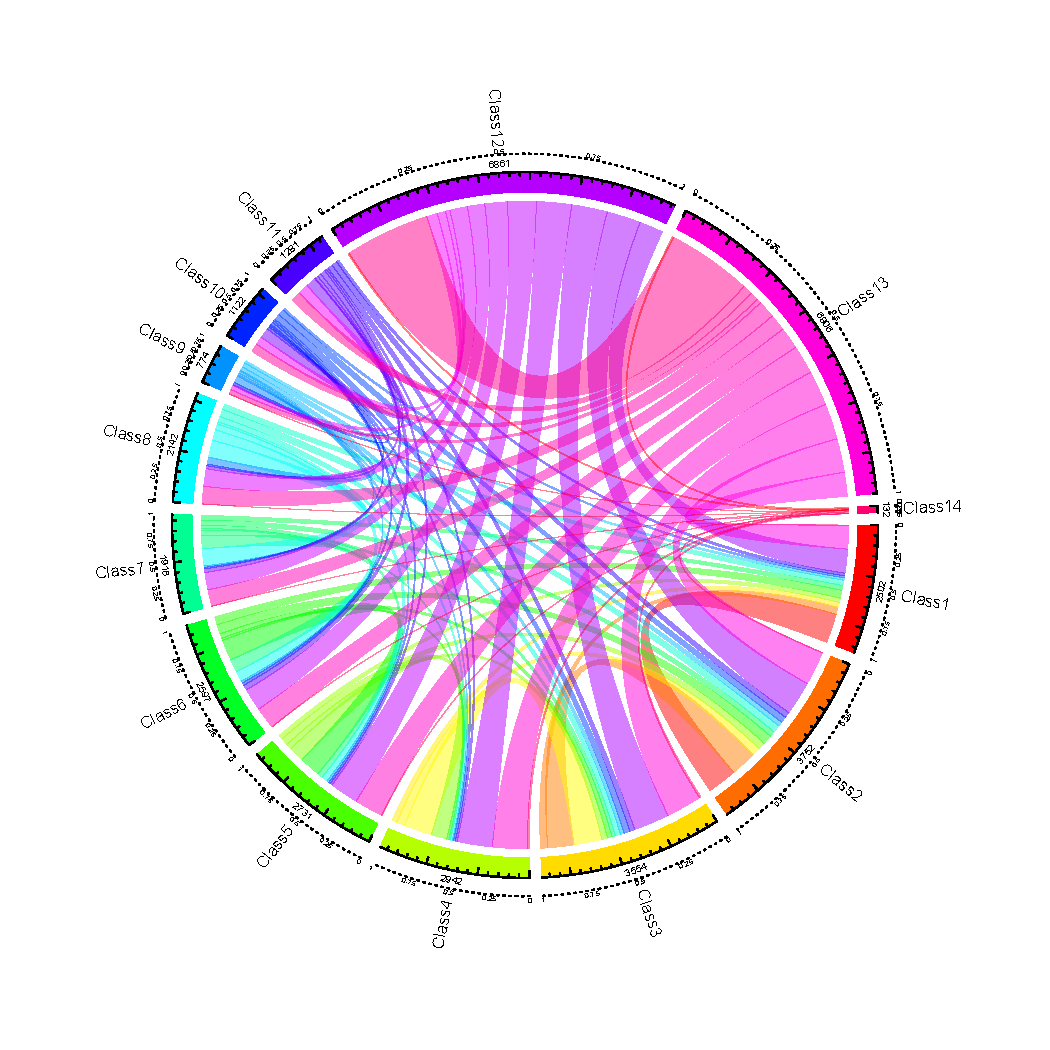
\includegraphics[width=\textwidth]{appendix/yeast_labelset}
    \caption{Yeast}
    \label{cooccurence:yeast}
  \end{subfigure}
  \begin{subfigure}[b]{0.48\textwidth}
    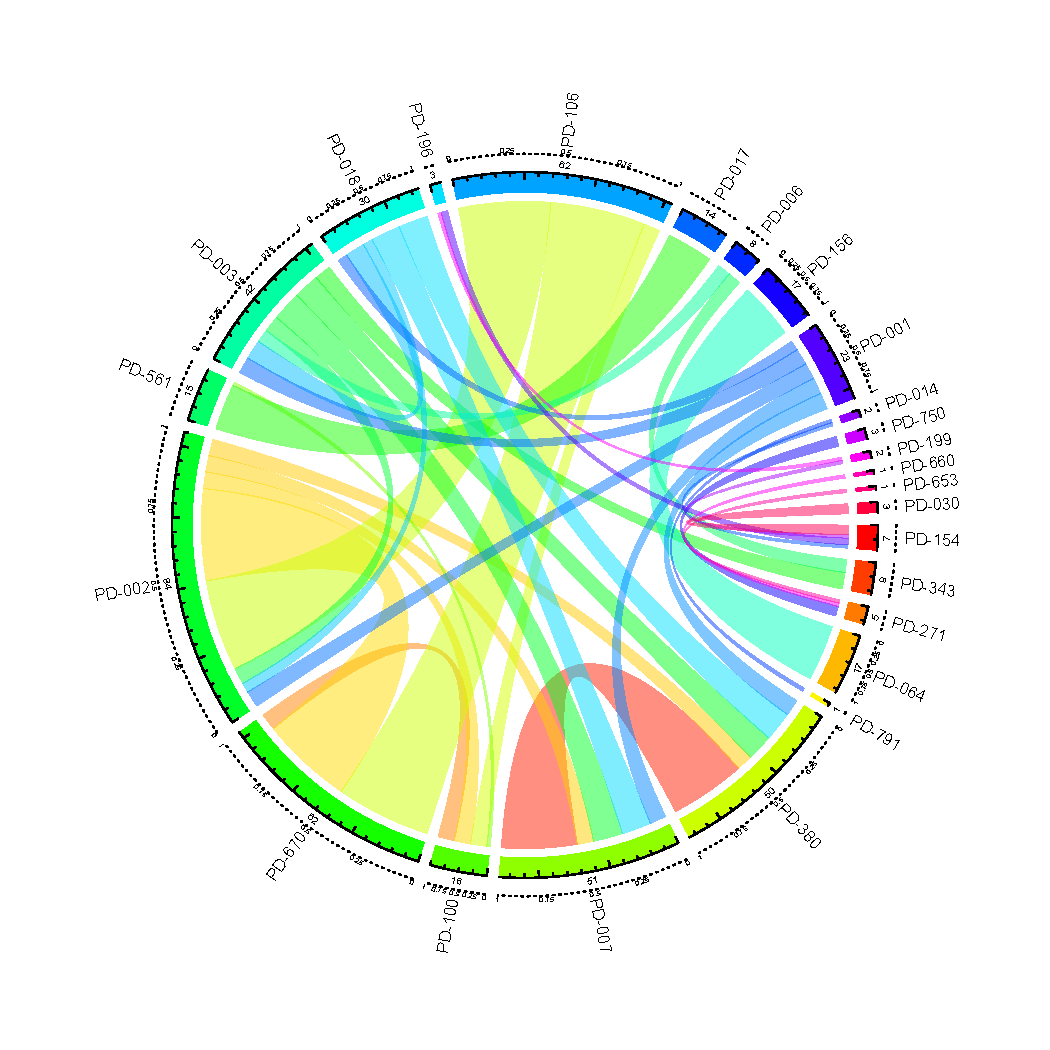
\includegraphics[width=\textwidth]{appendix/genbase_labelset}
    \caption{Genbase}
    \label{cooccurence:genbase}
  \end{subfigure}
  \caption{Cooccurence plot for protein benchmarks}
  \label{appendix:cooccurence}
\end{figure}

\par The work on multilabel data in general, not just in protein function
prediction, is a good area for further research (as addressed in Chapter
\ref{ConclusionsChapter}). It deals with problems not only in classification
but also  data imbalance and the like. For more information, we direct the
reader to the works of \cite{charte2015imbalance, charte2015mlsmote} and \cite{
charte2017dealing}

%=============================================================================
% PFPredict Package Appendix
% Copyright (c) 2018. Lester James V. Miranda
%
% This file is part of thesis-manuscript.
%
% thesis-manuscript is free software: you can redistribute it and/or modify
% it under the terms of the GNU General Public License as published by
% the Free Software Foundation, either version 3 of the License, or
% (at your option) any later version.
%
% thesis-manuscript is distributed in the hope that it will be useful,
% but WITHOUT ANY WARRANTY; without even the implied warranty of
% MERCHANTABILITY or FITNESS FOR A PARTICULAR PURPOSE.  See the
% GNU General Public License for more details.
%
% You should have received a copy of the GNU General Public License
% along with thesis-manuscript.  If not, see <http://www.gnu.org/licenses/>.
%
% Created by: Lester James V. Miranda <ljvmiranda@gmail.com>
%=============================================================================

\chapter{The `PFPredict' Package}
\label{AppendixPFPredict}

\par The main workhorse of this research is the PFPredict (\textbf{P}rotein
\textbf{F}unction \textbf{Predict}ion) software package. It is built on top of
Tensorflow and was written using Python 3.6 (also compatible for 2.7). It
contains the core implementation of the mutually-competitive autoencoder
architecture\footnote{
    PFPredict only contains the MC autoencoder. The stacked denoising
    autoencoder is a standard technique that can be implemented solely in
    Keras.
} and its corresponding prediction pipeline.

\section{Dependencies}

\par The table below describes the dependencies for this package. Again,
PFPredict was written in Python 3.6 (with 2.7 compatibility) and was tested
solely on Linux (Ubuntu 16.04) machines.

\begin{table}[!h]
\centering
\caption{Package dependencies}
\label{my-label}
\begin{tabular}{@{}rlp{0.65\textwidth}@{}}
\toprule
Package           & Version & Description                                    \\ \midrule
numpy             & 1.13.0  & matrix and linear-algebra library              \\
scipy             & 0.19.0  & scientific computation library                 \\
tensorflow        & 0.12.1  & tensor computation and neural network library  \\
keras             & 1.2.0   & high-level deep learning framework             \\
scikit-learn      & 0.18.1  & machine learning framework                     \\
scikit-multilearn & 0.0.5   & multilabel learning framework                  \\
future            & 0.16.0  & Python 2 to 3 interface                        \\
pyyaml            & 3.12.0  & easy-parsing of YAML files                     \\
matplotlib        & 1.3.1   & plotting library                               \\ \bottomrule
\end{tabular}
\end{table}


\section{Code Organization and Implementation}

\par There are three main modules in PFPredict: \texttt{utils},
\texttt{extractors}, and \texttt{pipelines}; there is also an auxiliary
\texttt{tests} module for unit tests. The \texttt{utils} module consists of
basic data input/output functionality, preprocessing, and console logging.
Next, the \texttt{extractors} module includes the \texttt{MCAutoencoder} class
for the mutually-competitive autoencoder. Lastly, the \texttt{pipelines} module
includes the \texttt{Pipelines} class where you can define your extractor and
classifier then run it on the data.

\subsection{The \texttt{MCAutoencoder} Class}

\par \texttt{MCAutoencoder} houses the implementation of the
mutually-competitive autoencoder. It inherits from Keras's \texttt{Layer} class
while the internals\textemdash winner-take-all and sparse operations\textemdash
are written in Tensorflow. It also follows \texttt{scikit-learn}'s standard
API: \texttt{fit()}, \texttt{transform(X)}, and \texttt{fit\_transform(X)}. A
UML for this design is seen in Figure \ref{uml:mcae}. 

\par Given a two-dimensional matrix \texttt{X} with each row as a protein
sample and each column a measurement, we can then use the following methods:

\begin{itemize}
    \item \texttt{fit(X)}: train the network using the initialized
        hyperparameters on the training set \texttt{X}. Learns the weight
        parameters of the network.
    \item \texttt{transform(X)}: use the learned weights to transform an input
        \texttt{X} into its latent representation. Returns the extracted
        features.
    \item \texttt{fit\_transform(X)}: higher-level abstraction that calls both
        \texttt{fit(X)} and \texttt{transform(X)} methods successively. Returns
        the extracted features.
\end{itemize}

\begin{figure}[!h]
  \centering
    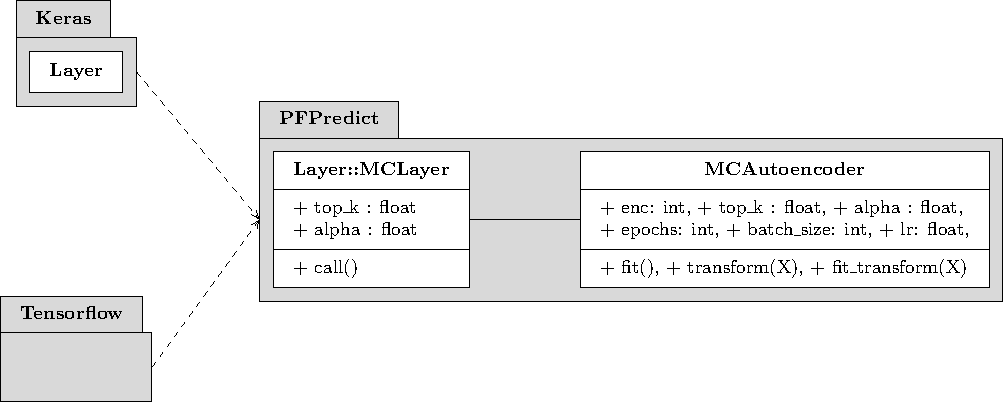
\includegraphics[width=0.85\textwidth]{appendix/uml_mcae}
    \caption{UML Diagram for the \texttt{MCAutoencoder} class}
  \label{uml:mcae}
\end{figure}

\par The main idea is to first initialize the \texttt{MCAutoencoder} class by
setting the hyperparameters, call the \texttt{fit(X)} method to the training
set, then call the \texttt{transform(X)} method to both training and test (or
validation) sets. The \texttt{transform(X)} method returns the extracted
features that we can now use for classification. The code sample below
illustrates this process.

\lstset{backgroundcolor=\color{gray!30}, basicstyle=\ttfamily,
breaklines=true}
\begin{lstlisting}[style=mypython, caption=Minimal example for extracting
protein features]
from pfp.extractors import MCAutoencoder
from pfp.utils import load_dataset

# Load Yeast dataset (we will not use the labels: unsupervised)
X_train, y_train, X_test, y_test = load_dataset('yeast', scale=True)
# Initialize the autoencoder with hyperparameters
feature_extractor = MCAutoencoder(enc=500, top_k=0.6, alpha=10.0)
# Fit model and learn network weights
feature_extractor.fit(X_train)
# Transform raw attributes into new features
X_train_new = feature_extractor.transform(X_train)
X_test_new = feature_extractor.transform(X_test)
\end{lstlisting}

\subsection{The \texttt{Pipelines} Class}

\par In order to run the experiments with ease, we designed a
\texttt{Pipelines} class that abstracts away the \texttt{MCAutoencoder} and
classifier. It takes a dataset, a feature extractor, and a multilabel
classifier as its input, and runs the whole prediction pipeline for a given
number of trials. It then returns a dictionary of scores for model evaluation.
The classifier object is obtained from the \texttt{scikit-multilearn}
library.\footnote{The author is also a collaborator in this project. Please see
\url{https://github.com/scikit-multilearn} for more information}

\begin{lstlisting}[style=mypython, caption=Minimal example for the prediction
pipeline]
from pfp.extractors import MCAutoencoder
from skmultilearn.problem_transform import BinaryRelevance
from sklearn.svm import SVC
from pfp.utils import load_dataset
from pfp.pipelines import Pipelines

# Load Yeast dataset (we will not use the labels: unsupervised)
yeast  = load_dataset('yeast', scale=True)
# Initialize the autoencoder with hyperparameters
mcae = MCAutoencoder(enc=500, top_k=0.6, alpha=10.0)
# Initialize the BR-SVM classifier
brsvm = BinaryRelevance(classifier=SVC(), require_dense=[False, True])
# Put extractor and classifier to pipeline and run
pipeline = Pipelines(extractor=mcae, classifier=brsvm, dataset=yeast)
scores = pipeline.run(trials=10)
\end{lstlisting}

\section{Miscellaneous Information}

\par This package is hosted in
\url{https://github.com/ljvmiranda921/pfpredict}, but, at this time of writing,
currently set to private. Continuous integration (CI) and deployment is set up
using TravisCI (\url{https://travis-ci.org/}), and the unit tests were written
using the \texttt{unittest} module.

%=============================================================================
% SVM Appendix
% Copyright (c) 2018. Lester James V. Miranda
%
% This file is part of thesis-manuscript.
%
% thesis-manuscript is free software: you can redistribute it and/or modify
% it under the terms of the GNU General Public License as published by
% the Free Software Foundation, either version 3 of the License, or
% (at your option) any later version.
%
% thesis-manuscript is distributed in the hope that it will be useful,
% but WITHOUT ANY WARRANTY; without even the implied warranty of
% MERCHANTABILITY or FITNESS FOR A PARTICULAR PURPOSE.  See the
% GNU General Public License for more details.
%
% You should have received a copy of the GNU General Public License
% along with thesis-manuscript.  If not, see <http://www.gnu.org/licenses/>.
%
% Created by: Lester James V. Miranda <ljvmiranda@gmail.com>
%=============================================================================

\chapter{Support-Vector Machines} 
\label{AppendixDistributed}

\par We have been mentioning Support-Vector Machines (SVM) as our pipeline's
classifier, yet have not provided any opportunity to discuss how it works. In
this chapter, we'll review the intuition behind SVMs, discuss how the
hyperparameters $C$ and $\gamma$ affect classification, then describe how we
implemented a distributed SVM for faster inference in multilabel data.

\section{Review and Intuition on SVMs}

\begin{wrapfigure}{r}{0.46\textwidth}
  \centering
    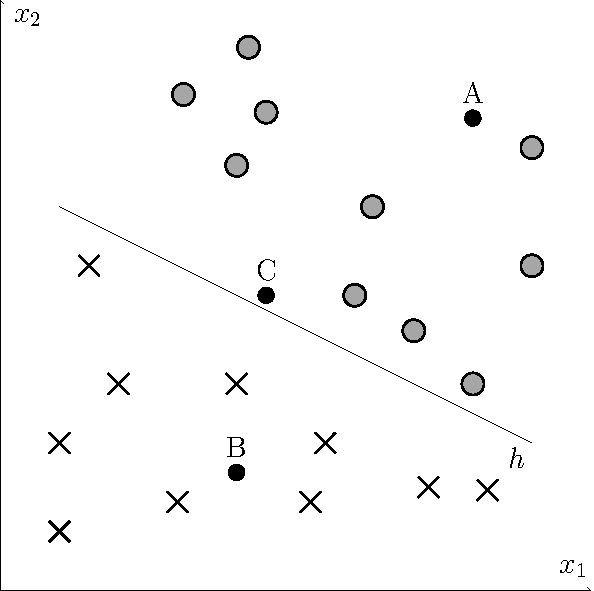
\includegraphics[width=0.45\textwidth]{appendix/svm_demo}
    \caption{Margin intuition for SVMs}
  \label{demo:svm}
\end{wrapfigure}

\par As an example, let's take a label $\lambda_1$ from our contrived protein
dataset (with only two features), and plot the samples on a Cartesian plane.
Figure \ref{demo:svm} shows the resulting plot.  The $\circ$ marks
represent protein samples that perform the function $\lambda_1$ (class 1),
whereas the $\times$ marks represent those that do not (class 0). We will also
draw a decision boundary $h$ that attempts to separate these classes.

\par If we query the unannotated sample $\mathbf{A}$, we can confidently infer
that it belongs to class 1. The same goes for sample $\mathbf{B}$, in this
case, class 0. However, we are on the fence with sample $\mathbf{C}$: it can
belong to class 1 according to the decision boundary, but it might as well be
class 0 if we nudge $h$ a bit. Our situation will be much better if we can
ensure that (1) our predictions are always \textbf{confident}, i.e. decision
boundary is maximally far from \textit{on-the-fence} samples, or
\textit{support vectors}, and that (2) they are \textbf{correct}, i.e., loss is
minimized. Ensuring that our decision-boundary makes confident and correct
predictions serves as the core machinery for the SVM classifier. We can write
this as an objective function $\gamma$:\footnote{\cite{ng2012support} gave a
thorough treatment of support-vector machines in his CS229 Lecture Notes. He
traces the development of SVMs from mere logistic regression up to Lagrangian
dualities and the kernel trick to solve the optimization problem.}

\begin{equation}
\begin{aligned}
\label{eqn:svm}
    & \underset{w,b}{\text{min}}
    & & \overbrace{\dfrac{1}{2}||w||^{2}}^{\mathclap{\text{confident}}} +
    C\overbrace{\sum_{i=1}^{m}{\xi_i}}^{\mathclap{\text{correct}}} \\
    & \text{s.t.}
    & & y^{(i)}(w^{T}x^{(i)} + b) \geq 1 - \xi_i, i=1,\dots,N \\
    &&& \xi_i \geq 0, i=1,\dots,N
\end{aligned}
\end{equation}

\par Without getting into the specifics of the objective function, we can see
that the hyperprameter $C$ is trying to balance our two goals: (1) ensuring
that the margin is far from the support-vectors by minimizing $||w||^{2}$, and
(2) checking that our predictions are correct. In addition, the parameters
$\{w, b\}$ are the same as the parameter $W$ learned during training in our
prediction pipeline (we simply let $b=w_0$). Lastly, we apply a kernel trick
to map our features with respect to the radial-basis function (RBF). Given two
samples $x$ and $z$, we write the RBF kernel as:

\begin{equation}
\label{eqn:kernel}
    K(x,z) = \text{exp} \left(-\gamma||x-z||^{2}\right)
\end{equation}

\par And thus we see the hyperparameter $\gamma$ that tries to consolidate the
\emph{effect} of each sample with respect to the other (measured in terms of
distance).\footnote{In some formulations, $\gamma=\dfrac{1}{\sigma^2}$} In the
next section, we will investigate the effect of the hyperparameters $C$ and
$\gamma$ in the behavior of our predictor.

\section{Practical Considerations for $C$ and $\gamma$ on the Decision Boundary}

\par From Equations \ref{eqn:svm} and \ref{eqn:kernel}, we can deduce the
effect of different hyperparameter settings to the decision boundary. The key
terms in this section are bias and variance, both refer to the generalizability
of the model.  Note that there is a tradeoff between bias and variance: too
high a bias underfits the model, while too high a variance overfits the model.

\begin{itemize}
    \item \textit{$C$ affects the way the margin is placed.} A \textbf{high}
        $\mathbf{C}$ will be motivated to predict more samples correctly than
        finding a large margin distance (high variance, low bias), but may fail
        to generalize well and perform poorly in the test set. On the other
        hand, a \textbf{low} $\mathbf{C}$ will strive to keep a good distance
        from support-vectors, but may suffer from severe underfitting (high
        bias, low variance).
    \item \textit{$\gamma$ affects the shape of the decision boundary.} The
        value of $\gamma$ controls each samples' area-of-effect. A
        decision-boundary with a \textbf{large} $\mathbf{\gamma}$ is only
        affected by the samples closest to it, creating a ``wiggly'' shape that
        conforms to the nearest samples (high variance, low bias). On the other
        hand, a \textbf{low} $\mathbf{\gamma}$ increases each samples'
        influence, thus even far-off samples are considered (high bias, low
        variance).
\end{itemize}

\par Figure \ref{demo:svm_hyperparams} demonstrates the effect of setting
different values for $C$ and $\gamma$ on a contrived binary dataset. We
randomly generated samples in two classes and ran SVM for different
hyperparameter settings then plotted the decision boundary for each
configuration. In the actual experiments, we first determined SVM hyperparameters
via grid search, then narrowed it down using fine random search.

\par We can see that a high-bias model ($C=1, \gamma=0.001$) underfits poorly
as it predicts everything as one class. On the other hand, a high-variance
model ($C=100, \gamma=1.0$) resembles the exact dumbell shape of the dataset.
Interestingly, the best performance for this simulation (3-fold
cross-validation) is from the high-variance model. This demonstration also
confirms our deductions: high $C$ or $\gamma$ values lead to high-variance models,
while low values lead to high-bias ones.


\begin{figure}[t]
  \centering
    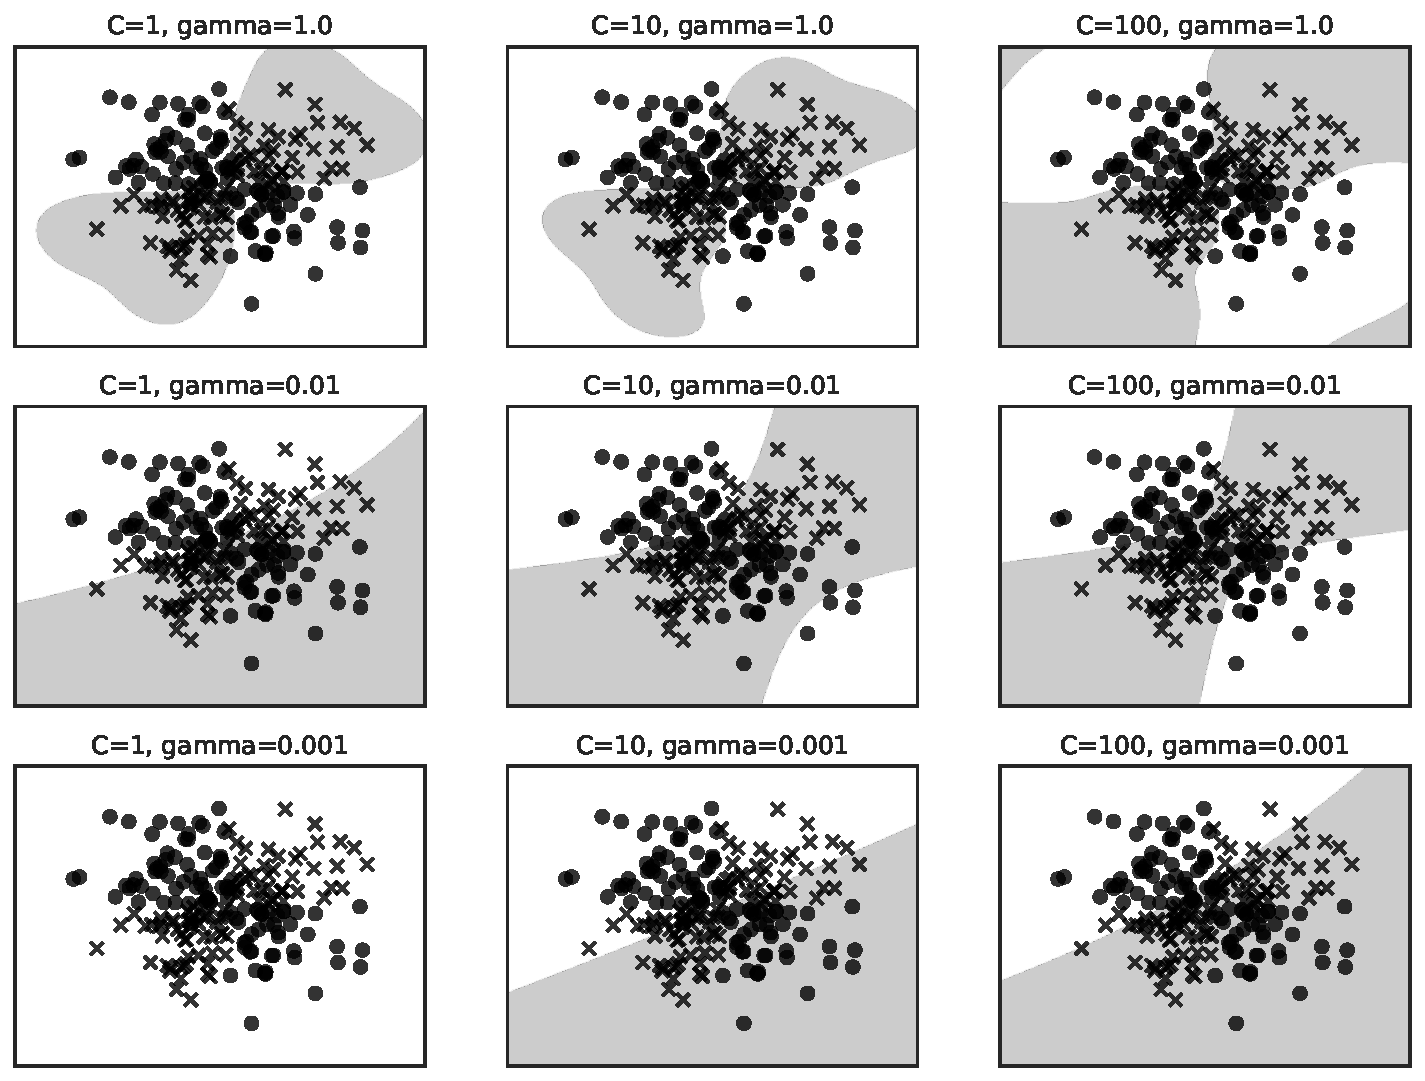
\includegraphics[width=0.85\textwidth]{appendix/svm_hyperparams}
    \caption{Effect of $C$ and $\gamma$ to the decision boundary}
  \label{demo:svm_hyperparams}
\end{figure}

\section{Distributed SVM Implementation}

\par In our work, SVM serves as the base classifier for the Binary-Relevance
(BR) algorithm. Recall that in BR, we take any ``off-the-shelf'' classifier and
train it $q$ times, where $q$ is the number of labels in the dataset. Most SVM
implementations have a time-complexity between $\mathcal{O}(N^2)$ and
$\mathcal{O}(N^3)$ (\cite{bottou2006support}).\footnote{We are using the
    \texttt{scikit-multilearn} library for BR and the \texttt{scikit-learn}
    library for SVM. Their SVM implementation is based on the \texttt{LIBSVM}
    solver by \cite{chang2011libsvm}.} 
With an overhead complexity brought by BR, our whole classifier algorithm can
take a long time to run.  Thus, we conducted a simple, distributed way of
training multiple SVM classifiers.

\par The main idea is to partition a dataset $\mathcal{D}$ into $K$ parts,
where $K \ll N$. We distribute each part into different jobs, i.e. each core of
the processor, and train it several times. Thus, given $q$ labels and $K$
partitions, we will have $K\cdot q$ smaller batches distributed on each core.
In practice, we limit the number of running cores to $10$ during
training.\footnote{The laboratory server's CPU has $40$ cores in total. This
can be confirmed by running \texttt{nproc --all} in the command line.} The
whole distributed process was implemented with the help of
\cite{varoquaux2010pipelines}'s \texttt{Pipelines} module (with
\texttt{multiprocessing} backend). Figure \ref{demo:distributed_svm} outlines
this process. When the \texttt{top} command is executed, we can see multiple
processes running inside the machine. A screenshot of this task is shown in
Figure \ref{demo:screenshot}.

\begin{figure}[t]
  \centering
    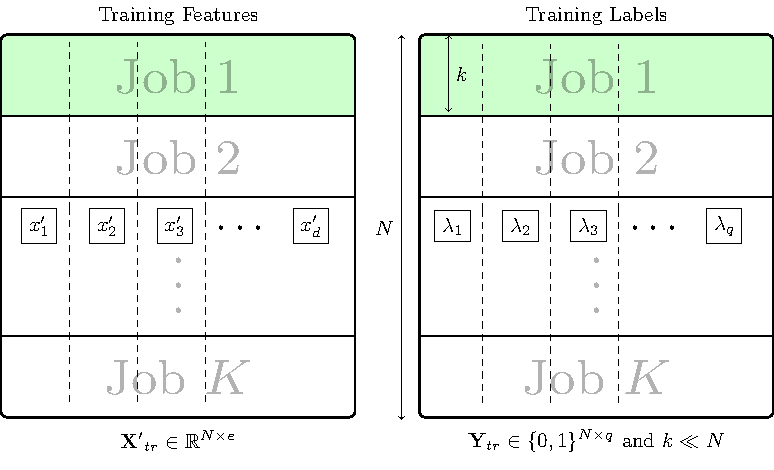
\includegraphics[width=0.70\textwidth]{appendix/distributed_svm}
    \caption[Distributed SVM training scheme]{Distributed SVM training
        scheme.\\ We partition the dataset into $K$ jobs, where $K\ll N$, and
    distribute it to different cores in our processor.}
  \label{demo:distributed_svm}
\end{figure}

\begin{figure}[!h]
  \centering
    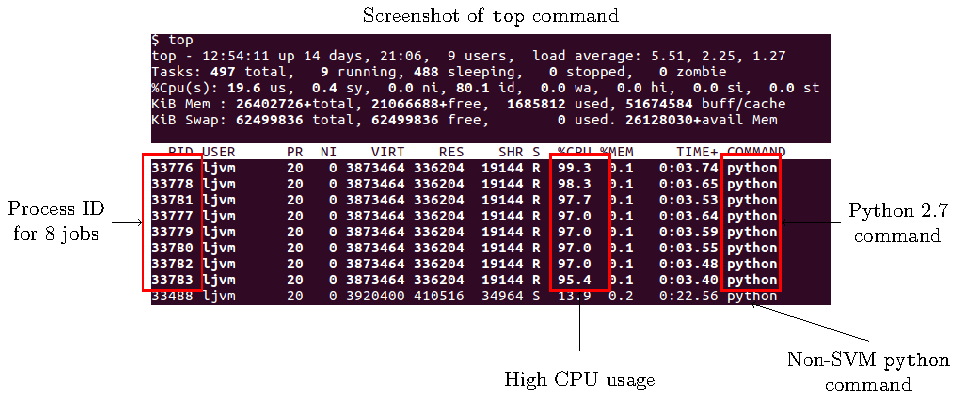
\includegraphics[width=0.95\textwidth]{appendix/parallel_compute}
    \caption[Screenshot of SVM jobs running in multiple cores]{Screenshot of
    SVM jobs running in multiple cores, $K=8$}
  \label{demo:screenshot}
\end{figure}

\par Lastly, we profiled this distributed approach by generating a toy multilabel
dataset and running it for different number of cores. For each step, we
measured the training time given different number of (1) samples, (2) features,
and (3) labels. Only the training time is measured because once the model is
fitted, inference is fast. The profiling results can be seen in Figure
\ref{demo:svm_profile}.

\begin{figure}[!t]
  \centering
    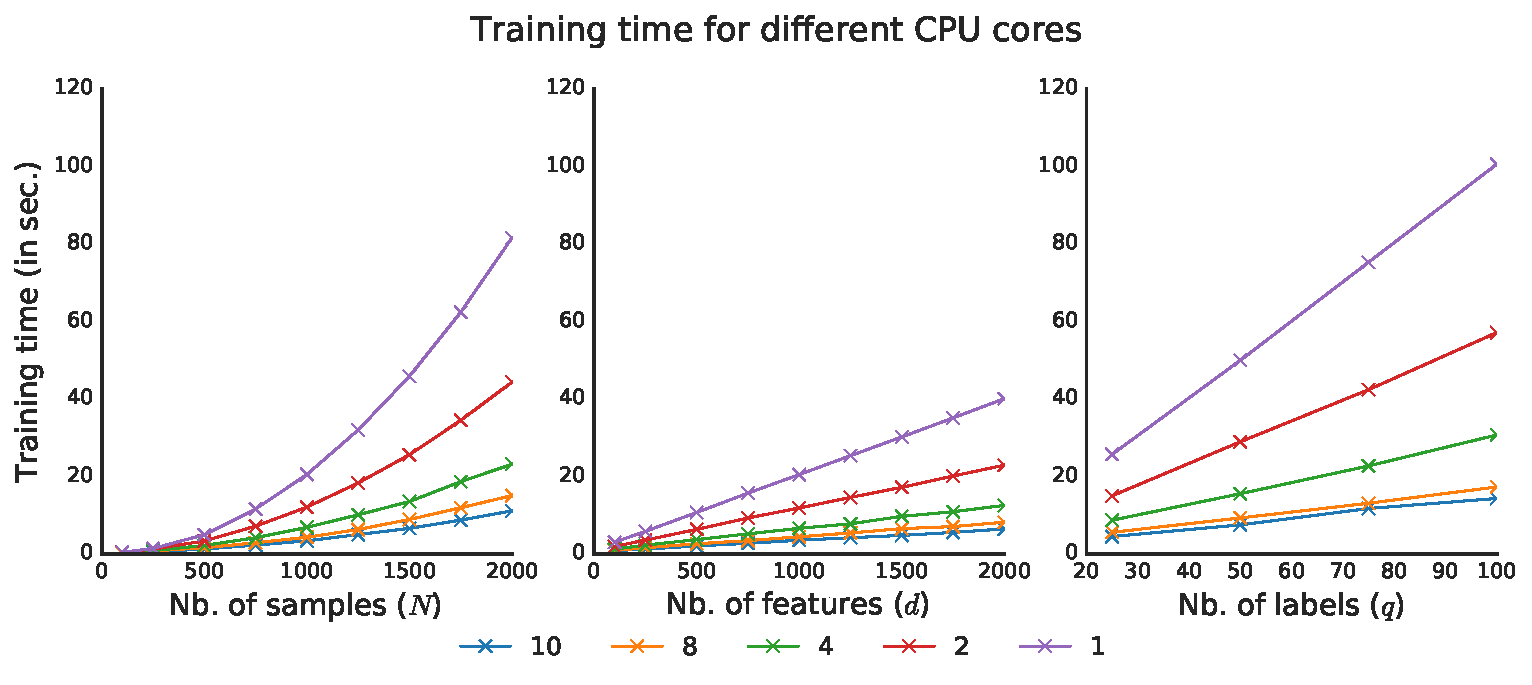
\includegraphics[width=0.95\textwidth]{appendix/svm_profile}
    \caption{Profiling results for SVM using different cores}
  \label{demo:svm_profile}
\end{figure}

\par It is evident that using the distributed approach reduces training time by
a large margin. The traditional approach ($K=1$) does not scale with large
datasets; it is more beneficial to use two or more cores for training. In
addition, we can also see the effect of different dataset sizes to the training
time. The curves in the leftmost plot shows an exponential relationship,
empirically validating the $\mathcal{O}(n^2)$ to $\mathcal{O}(n^3)$
time-complexity. On the other hand, the number of features ($d$) and labels
($q$) both exhibit a linear relationship with respect to the training time.
Either way, the curves above show that the distributed approach we have
implemented serves us in the long run. 


%------------------------------------------------------------------------------
%	BIBLIOGRAPHY
%------------------------------------------------------------------------------

\printbibliography[heading=bibintoc]

%------------------------------------------------------------------------------

\end{document}  
